% see: https://github.com/bamos/thesis/blob/master/thesis.tex

\documentclass{cmuthesis}
\usepackage[margin=1in]{geometry}
\usepackage[utf8]{inputenc}
\usepackage{amsmath}
\usepackage{amssymb}
\usepackage{amsthm}
\usepackage{bbm}
\usepackage{setspace}
\usepackage{xcolor}
\usepackage{bm}
\usepackage{esint}
\usepackage{hyperref}
\usepackage{float}
\usepackage{algorithm2e}

\usepackage{tikz}
\usetikzlibrary{decorations.pathreplacing,calligraphy}

\usepackage[
    backend=bibtex,
    style=authoryear,
    sorting=nyt,
    autocite=inline
]{biblatex}

\usepackage{graphicx}
\usepackage{subcaption}

\DeclareMathOperator*{\argmax}{arg\,max}
\DeclareMathOperator*{\argmin}{arg\,min}

\addbibresource{references.bib}

\newtheorem{definition}{Definition}
\newtheorem{example}{Example}
\newtheorem{proposition}{Proposition}
\newtheorem{condition}{Condition}
\newtheorem{theorem}{Theorem}
\newtheorem{lemma}{Lemma}
\newtheorem{corollary}{Corollary}
\newtheorem{conjecture}{Conjecture}

% \draftstamp{\today}{DRAFT}

\newcounter{fig}

% ----- 

\begin{document}
\frontmatter

\pagestyle{empty}

\title{{\bf Essays in Design Economics}}
\author{James Michelson}
\date{July 2024}
\Year{2024}
% \trnumber{???}

\committee{
\begin{tabular}{rl}
Kevin Zollman, Chair & \textit{Carnegie Mellon University} \\
Alexey Kushnir, Chair & \textit{Carnegie Mellon University} \\
Vincent Conitzer & \textit{Carnegie Mellon University} \\
\end{tabular}
}

% \support{}
% \disclaimer{}

% \keywords{philosophy of science, auction theory, computational social science, mechanism design, philosophy of economics}


\maketitle

\begin{dedication}
\normalfont{``Philosophers have hitherto only interpreted the world in various ways; the point, however, is to change it.''}\\
\hfill \normalfont{---Karl Marx,} \textit{Theses on Feuerbach}
\newline
\vspace{1cm}
\newline
\normalfont{``Yes, I do think we are simply the tellers of fables, but is that not wonderful?''}\\
\hfill \normalfont{---Ariel Rubinstein, `Dilemmas of an Economic Theorist'}
\end{dedication}


\begin{abstract}
This thesis contains two essays in philosophy of science on the value and application of economic theory and one essay in microeconomics on optimal multidimensional auction design.
 
On the topic of the value of economic theory in design economics, I propose a philosophical reformulation of scientific realism that is appropriate to the scientific domain of economics (chapter \ref{ch_fables}). In virtue of this formulation, I argue that economic theory explains the successes of design economics.

In chapter \ref{ch_reflexivity}, I advance a unified theory of observer effects across the social sciences, a problem I call \textit{reflexive measurement}. This theoretical understanding of the role of reflexivity extends more generally to all aspects of science including prediction and theorizing. I also examine the role of economic theory in addressing this problem.

In addition to these two philosophical contributions, chapter \ref{ch_auctions} is an extended exploration of optimal auction design in the multidimensional setting of a single good with multiple quality levels using simulations. This work examines whether the \textit{exclusive-buyer mechanism} is optimal and offers several conjectures concerning qualitative properties of optimal mechanisms in this analytically intractable setting.
\end{abstract}





\begin{acknowledgments}
I want to begin by thanking my friends and colleagues in Pittsburgh: Dejan Makovec, Brendan Fleig-Goldstein, Bele Wollesen, Mason Broxham, Andrew Warren, Gal Ben-Porath, Nil-Jana Akpinar, Fernando Larrain, Zeyu Tang, Sam Mark, Carly Medina, Max Siemers. Without you this journey would have been immeasurably worse.

My debt of gratitude also extends those to who were a little further away: Marina Dubova, Tim Cejka, Adrianna Kayla Lee, Agne Sabaliauskaite, Giovanna Vitelli, Hannah Schigutt, John Davis, Zac Laporte, Ola Topczewska, Marina Michelson, Rawle Michelson. Your support was invaluable.

% Robin Mejia was instrumental in developing the examples for chapter \ref{ch_reflexivity}

I have also benefited enormously from faculty who've advised and mentored me throughout my time in Pittsburgh. David Danks was a fantastic supervisor for my Masters degree and continued to offer sage advice throughout my time at CMU. David Childers has been source of invaluable help and patience as I've explored philosophical problems in economics well beyond the scope of this thesis. Vincent Conitzer was able to offer incredible advice and feedback in \textit{both} auction theory and philosophy. Kevin Zollman has been my supervisor throughout my time at CMU and has been as unfailing in his generosity as he has been insightful in his feedback. Finally, Alexey Kushnir took a gamble on a philosopher with a programming habit early in my PhD. Without that decision, this thesis would not exist.

Pittsburgh has been a wonderful place to complete a PhD. I am grateful for the flora and fauna responsible for keeping me healthy and happy throughout my time here: from Greta, the groundhog living in my backyard, to peaceful summer evenings spent Schenley Park. Additionally, special thanks to Akshay Venkatesh, Lindsey Graff, Vyas Sekar, Christopher Philips, and Frank Pfenning. I pray your squash game lives to regret my departure.
\end{acknowledgments}


\pagestyle{plain}

\tableofcontents
\addtocontents{toc}{\vspace*{-1cm}}
% \listoffigures
\addtocontents{lof}{\vspace*{-1cm}}
% \listoftables
% \listofalgorithms

\mainmatter

\chapter{Introduction}

\section{Motivation}

Suppose a famous auction house like Sotheby's\footnote{\url{https://www.sothebys.com/en}} wishes to maximize its profits selling a work of art. Which auction format should it use? Auctions can be \textit{open-bid} or \textit{sealed-bid}, depending on whether bidders must reveal their bids publicly. An auction can also be \textit{single-round} or \textit{multi-round}, where bidders are allowed to bid multiple times, as in the case of English\footnote{\url{https://en.wikipedia.org/wiki/English_auction}} or Dutch\footnote{\url{https://en.wikipedia.org/wiki/Dutch_auction}} auctions. Multiple goods may be sold, sometimes packaged or \textit{bundled} together for a discount. \textit{Reserve prices} for these goods can be posted so that a seller will only sell if bids are above them. In \textit{all-pay} auctions, all bidders are required to pay irrespective of whether they submit the winning bid. Additionally, auctions can even require bidders pay an amount different than their bid, as in the case of a \textit{second-price} auction\footnote{Most commonly contrasted with a \textit{first-price} auction, where the bidder with the highest bid wins the good(s) and pays the value of their bid.}, where the bidder with the highest bid pays wins the good(s) but only pays the value of the second highest bid.

Perhaps surprisingly, it turns out this question has an associated deep body of economic theory, stretching back to Nobel Laureate William Vickrey's \autocite*{vickrey1961} seminal research demonstrating the revenue equivalence of first and second-price auctions. Auction theory---more generally, the theory of \textit{mechanism design}---has illuminated many facets of the problem of designing auctions. Theoretical work has extended Vickrey's famous result, characterizing the entire class of profit-maximizing auctions for selling a single good \autocite{myerson1981optimal}. We know that if multiple goods are sold offering selling them together \autocite{adams1976} or offering a lottery, where the bidder is unsure which good they end up with in the event they win \autocite{thanassoulis2004}, can increase profits. Theoretical work has even extended our understanding of `rational' behavior in auctions \autocite{li2017}, adding to our scientific arsenal of concepts that we can use to characterize how people will respond to different institutional designs. These are only a few examples from the decades of research in theoretical economics that applies to designing auctions.

This theory also applies much more widely than one might initially guess. An auction can be represented mathematically by a pair of functions\footnote{A comprehensive model of multidimensional auction design relevant to the microeconomic portion of this thesis is introduced in section \ref{sec_model}.}. An \textit{allocation function} maps bids to outcomes. A \textit{transfer function} maps bids to payments. With this pair of functions it is possible to characterize the wide range of variations in auction format introduced above. Moreover, this mathematical representation covers a surprisingly wide range of design problems. Parallels can immediately be drawn to the problem of \textit{price screening} faced by a monopolist\footnote{The problem of price screening is commonly known as \textit{second-degree price discrimination}, where a seller offers a range of options to buyers in order to reveal buyers' private information concerning the value of the seller's goods.}. Any bilateral trading platform (e.g., a stock market or exchange) can be characterized as a \textit{double auction} with multiple buyers and sellers, offering an alternative perspective on the design of markets. The theory of auction design has even been applied to the problem of data acquisition and survey sampling \autocite{roth2012surveys}, an example covered in more detail in chapter \ref{ch_reflexivity}.

What is the scientific value of this body of economic theory? Is it actually useful for designing institutions and policy-making? Economists and philosophers of science are divided on this question. Well-known, award-winning microeconomic theorists like Ariel Rubinstein believe economic theory merely amounts to a collection of fables \autocite{rubinstein2012} whereas other equally well-known, award-winning microeconomic theorists assert that this kind of scientific theory has predictive value and sharpens the intuitions of economists working on these problems \autocite{roth2019}. Philosophers of science are no less split, with some arguing that economic theory played an incredibly limited role in some of the major successes of auction design in the 1990s \autocite{nikkhah2008} and others asserting this kind of theory is true in a strong, ontological sense \autocite{ross2008}.

This thesis represents a philosopher of science's attempt to better understand a body of scientific theory combined with an attempt to contribute to it. The overarching goal is to illuminate the value and uses of economic theory for questions of design. The scientific portion of this thesis contributes to our theoretical understanding of auction design. The philosophical orientation of this thesis is prescriptive. The philosophical conclusions of this thesis directly entail recommendations regarding how to improve science. Thus, the novel philosophical contributions of this thesis are intended to be relevant for economists and social scientists interested in the foundational problems that concern the study of human behavior.


% \section{Contributions


\section{(A Very Brief) Introduction to Design Economics}\label{intro_sec_whatis}

Design economics is both a collection of institutional design problems as well as an approach to doing economics\footnote{See section \ref{fable_sec_design} for an extended introduction to this topic, along with consideration of two major empirical successes from the 1990s: the Federal Communication Commision's (FCC) 1994 radio spectrum auction and the National Resident Matching Program's (NRMP) redesign of the matching algorithm in 1996.}. Economist Al Roth has called design economics ``the part of economics intended to further the design and maintenance of markets and other economic institutions'' \autocite[1341]{roth2002}. It is often used synonymously with `market design'. At its core, the theoretical content of design economics models the choice a principal (designer) makers concerning how to design an institution to achieve some goal. Common goals include profit maximization (optimality), welfare maximization, efficiency, stability, and equity. Oftentimes, this work is applied in orientation. Economists increasingly consult on questions of policy and empirical and computational work play a prominent role alongside economic theory (see, for first-hand accounts of this phenomenon, \cite{binmore2002, roth2019, sönmez2023minimalist}). 

What are some examples of institutional design problems tackled by economists working in design economics? Auction design, introduced above, is a core topic in design economics. Both empirical and theoretical work in economics tries to understand the trade-offs that come with choosing one type of auction format over another. Matching problems are another major topic. These concern problems like matching students to schools, new doctors to hospitals, and organs to transplant recipients. The flexibility of economic theory in this domain means that it can be applied well beyond the setting that motivated its development. As mentioned above, auction theory also applies to problems of price discrimination and data acquisition, a topic that was pioneered by computer scientists (see, for example, \cite{roth2012surveys, cai2015}). Although economists aided policymakers on questions of institutional design in the 1990s, since then computer scientists have been increasingly involved in applying economic theory to problems in and adjacent to computer science\footnote{Computer scientists have also been at the forefront of studying computational aspects of economic theory (see, for example, \cite{nisan2007algorithmic}).}. Although the canonical problems of auction design and matching markets were responsible for establishing the domain of design economics, its successes have broadened its scope of application and attracted scientists from neighboring disciplines.

The intellectual origins of design economics can be traced to the 1960s and 70s. Early work on auctions \autocite{vickrey1961} and matching mechanisms \autocite{gale1962} blossomed into substantial theoretical literature in mechanism design and matching theory. Mechanism design, in the spirit of Hurwicz \autocite*{hurwicz1972}, became a discipline in its own right, which now boasts its own specialized journal, the \textit{Review of Economic Design} (created in 1994). A similar story exists for the development of matching theory. Ultimately, both of these disciplines blossomed alongside related empirically oriented literature on the outcomes of particular forms of institutional design\footnote{See, for example, discussions by Roth \autocite*{roth2002} and Myerson \autocite*{myerson2008}.}. To understand the theoretical orientation of this type of scientific modeling, one of the founders of mechanism design, Leonid Hurwicz, has described it as follows:
\begin{quote}
	in a design problem, the goal function is the main given, while the mechanism is the unknown. Therefore, the design problem is the inverse of traditional economic theory, which is typically devoted to the analysis of the performance of a given mechanism. \autocite[30]{hurwicz2006designing}
\end{quote}
\noindent Though economic theories of design economics do examine the performance of particular institutions, much theoretical work takes place in the same vein that Hurwicz outlined. As I will show in chapter \ref{ch_fables}, these approaches are complementary.

As noted above, in design economics empirical and computational work are seen as ``natural complements'' \autocite[1363]{roth2002} to theory. This has led to what some economists have called the `engineering approach' to questions of institutional design. Al Roth has elaborated on this approach by way of analogy with the construction of suspension bridges:
\begin{quote}
	The simple theoretical model in which the only force is gravity, and beams are perfectly rigid, is elegant and general. But bridge design also concerns metallurgy and soil mechanics, and the sideways forces of water and wind. Many questions concerning these complications can’t be answered analytically but must be explored using physical or computational models. These complications, and how they interact with the parts of the physics captured by the simple model, are the domain of the engineering literature. \autocite[1342]{roth2002}
\end{quote}
\noindent The key idea behind the engineering approach is that computation and experimentation ``fill[] the gaps between theory and design'' \autocite[p1374]{roth2002}. Computational methods analyze settings that are too complex to solve analytically and laboratory experiments offer predictions about how people will behave in these environments. This kind of approach motivates the use of simulations in chapter \ref{ch_auctions} of this thesis.

The rise of design economics has been tied to a change in perspective in how economists view their subject matter. This change has even recently been lamented by economic theorists:
\begin{quote}
    If I had to name one major shift in the sensibilities of economic theorists in the past half century, a prime candidate would be the way we conceptualize markets---from quasi-natural phenomena admired from afar to man-made institutions whose design can be tweaked by economist-engineers. \autocite[p137]{spiegler2024}
\end{quote}
\noindent I believe this change reflects progress in the science of economics. The turn away from contemplating man-made institutions as ``quasi-natural phenomena'' characterizes a step in the evolution of the `dismal science' of economics towards a better understanding of our (socially constructed) world. I hope to convince the reader that not only is the theoretical contents of this emerging scientific domain philosophically interesting in its own right but also that it can be fruitfully applied to address foundational problems in other areas of social science.


\section{Structure of the Thesis}

This thesis consists of three chapters: two in the philosophy of science, one focusing on economic theory in design economics (chapter \ref{ch_fables}) and the other on statistics in social science (chapter \ref{ch_reflexivity}), as well as an additional chapter in auction theory (chapter \ref{ch_auctions}). The chapters in this thesis can be seen as answering the following related questions:

\begin{itemize}
	\item \textit{`What is the scientific value of economic theory in design economics?'} (chapter \ref{ch_fables})

	\item \textit{`What is an example of a theoretical contribution in design economics?'} (chapter \ref{ch_auctions})

	\item \textit{`What other problems might this body of theory help with?'} (chapter \ref{ch_reflexivity})
\end{itemize}

\noindent Although each chapter is self-contained, the two chapters in philosophy of science are ordered in the following way: the conclusion of chapter \ref{ch_fables} on the value of economic theory in design economics---that economic theory explains the successes of design economics---strengthens the case for its application to problems of reflexive measurement in chapter \ref{ch_reflexivity}. The recommendation to apply the theory of mechanism design to the problem of designing incentive-compatible measurements (\ref{sec_reflex_mechdes}) follows from the conclusion concerning the value of this theory.

Chapter \ref{ch_fables} offers a \textit{minimal non-fable} account of economic theory in design economics. The goal of this chapter is to offer a philosophical refutation of the position that economic theory does not ``produce conclusions of real value'' \autocite[37]{rubinstein2012}. My argument draws inspiration from a classic philosophical argument that argues for the truth of scientific theories in virtue of their success---the \textit{no-miracles} argument for scientific realism \autocite{putnam1975}. However, this chapter adapts arguments for realism to scientific domains where notions of truth are a ``non-starter'' \autocite[328]{alexandrova2009}. Instead of arguing for the strong conclusion concerning the truth of economic theory in design economics, I argue for a much weaker thesis: economic theory explains the successes of design economics. I develop an account of the economic theory of design which I believe best accounts for the recent empirical successes of economics\footnote{These successes are outlined in more detail in section \ref{fable_sec_design} and a brief overview of design economics is provided below (section \ref{intro_sec_whatis}).}. Unlike existing philosophical accounts of the role of economic theory in design economics (see, for example, \cite{alexandrova2009, ross2008}) the argument developed here is sensitive to contemporary contributions by economists and computer scientists as well as captures the subtle differences in the kinds of theory used to inform questions of institutional design.

% The scientific contributions of this thesis concern theoretical questions of optimal auction design in the multidimensional setting of a single good with multiple quality levels. These are covered in chapter \ref{ch_auctions}. These contributions fall squarely in the tradition of design economics, which views computation and experiment as ``natural complements'' \autocite[1342]{roth2002} to theory. The contributions are generative in that they ``suggest[] an agenda for theoretical work'' \autocite[1363]{roth2002}. Using simulations, the optimality of the \textit{exclusive-buyer mechanism}\footnote{The exclusive-buyer mechanism is formally defined in section \ref{subsec_ebm}. For a review of related work, see the literature review in section \ref{sec_litreview}.} is explored alongside other conjectures concerning qualitative characteristics of profit-maximizing mechanisms in this multidimensional setting. Surprisingly, I find the exclusive-buyer mechanism is optimal in settings where randomization is not required for profit maximization. Additionally, I find that the \textit{exclusion region}---the measure of the type space which does not receive the good in equilibrium---does not change with the number of bidders and is sometimes measure zero.

The scientific contributions of this thesis can be found in chapter \ref{ch_auctions}. These concern developing an improved understanding of optimal auction design in the multidimensional setting of a single good with multiple quality levels. Optimal multidimensional auction design problems are notoriously difficult to solve analytically and for this reason, the setting is explored using simulations. These contributions fall squarely in the tradition of design economics, which views computation and experiment as ``natural complements'' \autocite[1342]{roth2002} to theory. Using simulations, the optimality of the \textit{exclusive-buyer mechanism}\footnote{The exclusive-buyer mechanism is formally defined in section \ref{subsec_ebm}. For a review of related work, see the literature review in section \ref{sec_litreview}.} is explored alongside other conjectures concerning qualitative characteristics of profit-maximizing mechanisms in this multidimensional setting. Surprisingly, I find the exclusive-buyer mechanism is optimal in settings where randomization is not required for profit maximization. Additionally, I find that the \textit{exclusion region}---the measure of the type space which does not receive the good in equilibrium---does not change with the number of bidders and is sometimes measure zero. The contributions are generative in that they ``suggest[] an agenda for theoretical work'' \autocite[1363]{roth2002} and can be used to guide future theoretical research on optimal multidimensional auction design.

The final substantive chapter of the thesis advances a general philosophical account of observer effects in the social sciences (chapter \ref{ch_reflexivity}). My account unifies almost a century of sustained research on this topic by both scientists and philosophers. In my view, observer effects can be understood as problems of \textit{reflexive measurement}, which occur when people are aware of their status as objects of scientific investigation. Viewed at a sufficient level of philosophical abstraction, this characterization not only recovers well-known problems in the social sciences like `Goodhart's Law' and the \textit{Hawthorne effect} but also sheds new light on how to overcome them. A typical understanding of measurement error will fail to account for the distribution shift caused by a reflexive measurement. The conclusions of chapter \ref{ch_fables} facilitate a connection to recent developments in theoretical computer science in the field of \textit{incentive compatible learning}. I argue that the economic theory of design economics can address problems of reflexive measurement where other ascientific, ``purely statistical'' \autocite[319]{marget1929} approaches fail to do so. 

% The conclusion of chapter \ref{ch_fables} concerning the value of economic theory in the context of design is directly applicable in chapter \ref{ch_reflexivity}, which concerns developing a general philosophical account of observer effects in social science. The problem of \textit{reflexive measurement} characterizes any science where the agents who are under investigation are aware of their status as a target of scientific inquiry. This problem has been widely studied for almost a century, drawing attention from noted economists \autocite{morgenstern1928}, sociologists \autocite{merton1948}, and philosophers of science \autocite{popper1953}. This chapter explicitly connects this foundational problem in social science with contemporary applied statistical practice as well as recent developments in theoretical computer science in the field of \textit{incentive compatible learning}. I argue that the economic theory of design economics can address problems of reflexive measurement where other ascientific, ``purely statistical'' \autocite[319]{marget1929} approaches fail to do so. 



% ---- old `structure of thesis section



% Chapter \ref{ch_fables} directly addresses Rubinstein's \autocite*{rubinstein2006, rubinstein2012} contention concerning the role of economic theory as a collection of fables. The chapter puts forward a \textit{minimimal non-fable} account of economic theory for the domain of design economics. The scope of this chapter is deliberate. Insofar as design economics boasts a number of impressive achievements, these success stories render questions concerning the usefulness of economic theory increasingly urgent. Does economic theory explain these successes? I believe so. By adapting a \textit{no-miracles} argument \autocite{putnam1975} for scientific realism, I argue that it is unlikely (miraculous) that the theory common to these success stories does not, in part, explain their success. Rubinstein's \textit{theory-as-fable} account is found untenable. The particular \textit{projective} quality \autocite{guala2001} of economic theory in this domain is explored to illuminate how economic theory might serve to bring about these successes

% With a philosophical argument for the scientific value of economic theory in design economics firmly in place, chapter \ref{ch_auctions} tackles the question of optimal multidimensional auction design in the setting of a single good with multiple quality levels. In the spirit of design economics explored in the previous section, simulations are used to explore this analytically intractable setting. These simulations are derived from modifying the plane-cutting algorithm developed by Belloni et al. \autocite*{belloni2010multidimensional} to improve performance and facilitate exploration of a wide variety of settings. In particular, I explore the performance of the \textit{exclusive-buyer mechanism}. This is a deterministic mechanism that allocates the good according to a multidimensional analog of the single-dimensional virtual value (see section \ref{subsec_ebm} for details). I find the simple exclusive-buyer mechanism not only well approximates the revenue from the optimal mechanism but the interim allocations are qualitatively similar to those of the optimal mechanism when the optimal mechanism is deterministic. (Surprisingly, deterministic mechanisms are often optimal in multidimensional settings). Additionally, two conjectures are investigated concerning the measure of types excluded by the optimal mechanism in equilibrium. 

% The final chapter \ref{ch_reflexivity} offers a unified philosophical account of observer effects in social science. When agents are aware their behavior is subject to scientific inquiry they often act in ways that render measurements of them unreliable. This is the problem of \textit{reflexive measurement}, the central topic of this chapter. In order to develop this novel account, I provide a general characterization of reflexivity which encompasses the full scope of scientific practice: theorizing, prediction, measurement, etc. The characterization captures the insights of contemporary philosophers of science working on reflexive prediction alongside observations by scientists grappling with observer-type effects in the course of their research.






% ------ first attempt

% \section{Motivation}

% Two fundamental questions animate this thesis. First, `\textit{How should a philosopher's scientific investigations constrain their philosophy?}' Second, `\textit{How should a scientist's philosophical convictions inform the way they practice science?}'. Although neither of these questions are addressed directly, they have indirectly motivated the entirety of this thesis. Thus, this work reflects a philosopher's extended scientific engagement with microeconomic theory, particularly auction design, and a philosophical attempt to understand the value of this theory.

% Like Marx, my philosophical inclinations towards science are unwaveringly prescriptive. Insofar as a `better' science can be identified and argued for, the path to get there is part of the conclusion of the argument. This is reflected in both chapters on the philosophy of science and mechanism design. In Chapter \ref{ch_fables}, I propose an account of economic theory in the discipline of `design economics' \autocite{roth2002} that recovers the prescriptive elements of design---what philosopher of science Francesco Guala \autocite*{guala2001} has called \textit{projective} theory. In my philosophical view, the attractive scientific quality of this kind of economic theory is its constructive orientation toward designing a better world. Arriving at this conclusion, however, was entirely incidental. Without my work in multidimensional auction design, I would never have understood the significance of the perspective of design. 

% Seeing the social world through the eyes of economic design was a revelation for me. This nascent sensibility has been (unfortunately, in my opinion) lamented by economic theorist Ran Spiegler \autocite*[p137]{spiegler2024}, who sagely writes:
% \begin{quote}
%     If I had to name one major shift in the sensibilities of economic theorists in the past half century, a prime candidate would be the way we conceptualize markets---from quasi-natural phenomena admired from afar to manmade institutions whose design can be tweaked by economist-engineers. 
% \end{quote}
% \noindent This ``shift in sensibility'' opened my eyes to how mechanism design could be applied to problems I formerly encountered as a data scientist working in political analytics. The techniques of \textit{incentive compatible learning} represent, in my eyes, a radical new scientific approach to tackling the problem of reflexivity or performativity---what social scientists would call instances of the \textit{Hawthorne Effect} (see \cite{landsberger1958}). This is covered in chapter \ref{ch_reflexivity}. Here, my work on auction design was directly responsible for changing my convictions about how to overcome the scientific problem of misaligned incentives in measurement.

% This thesis is also partly a scientific enterprise. The work on optimal multidimensional auction design in chapter \ref{ch_auctions} falls very much in the vein of `design economics' which is also a target of philosophical investigation. Building on the work of Belloni et al. \autocite*{belloni2010multidimensional}, I developed a novel algorithm to explore the qualitative features of optimal mechanisms in multidimensional settings that are analytically intractable. This project is informed by the philosophical attitude towards simulation which views it as a ``natural complement'' \autocite[1342]{roth2002} to theory. This work is generative. Its aim, much in the vein of other work in design economics, is to better understand a complex theoretical setting with an eye to uncovering simple mechanisms, unexpected features, and ``suggest an agenda for [future] theoretical work'' \autocite[1363]{roth2002}.

% Contrary to the claims of Ariel Rubinstein, I disagree economic theory amounts to a mere `collection of fables' \autocite{rubinstein2006,rubinstein2012}. Again, like Marx, I find such a conviction entirely wrongheaded. (So much so I struggle to contain my incendiary writing). To decry the role of theory as fable is to remove our ability to evaluate it in virtue of its ability to materially improve our lives. And insofar as the profession of economics continues to champion the success of theory Rubinstein's contention places it beyond reproach---\textit{all} theory is fable, there is no `better' or `worse'. I believe such a position can only stymie progress in economics. I hope to convince the reader that economic theory, in particular mechanism design, can be used to design a better world. Moreover, the basis for this conviction is rooted not in ethics or political philosophy but instead in an understanding of philosophy of science.




% \section{(A Very Brief) Introduction to Mechanism Design}

% Before outlining the structure of this thesis in more detail it is helpful to briefly describe the topic of mechanism design. At a minimum, philosophers of science ought to better understand the body theory that is the target of philosophical investigation. The particular context of multidimensional auction theory relevant to the scientific portion of this thesis is introduced in much greater detail in section \ref{sec_model}. 

% \textit{Mechanism design} is a type of game theory that deals with games of incomplete information. It is often lumped together with the field of \textit{adverse selection}, which studies how a principal interacts with an agent with unknown characteristics (see, for details, \cite{salanie2005economics}). Canonical examples of adverse selection problems are those of insurance policy: how much should I charge you for health insurance if I am unsure about your smoking habits? Mechanism design, however, is more generally concerned with designing games that implement a social choice function. A \textit{mechanism} is ``essentially a set of rules to govern the interactions of the parties'' \autocite[21]{milgrom2004}. One of the founders of mechanism design, Leonid Hurwicz, has described the type of scientific modeling as follows: 
% \begin{quote}
% 	in a design problem, the goal function is the main given, while the mechanism is the unknown. Therefore, the design problem is the inverse of traditional economic theory, which is typically devoted to the analysis of the performance of a given mechanism. \autocite[30]{hurwicz2006designing}
% \end{quote}
% \noindent Most commonly, though by no means exclusively, mechanism design is concerned with designing economic institutions like auctions, markets, and other trading platforms\footnote{See Al Roth's \autocite*{roth2002} introduction to design economics for an overview of common applications of mechanism design.}. However, mechanism design extends to domains in political science and even to problems in statistics, as are considered in more detail in chapter \ref{ch_reflexivity}.

% Crucially, as a body of scientific theory,
% \begin{quote}
% 	[t]he distinguishing characteristic of the mechanism-design approach is that the principal is assumed to choose the mechanism that maximizes her expected utility, as opposed to using a particular mechanism for historical or institutional reasons. \autocite[243]{fudenberg1991game}
% \end{quote}
% \noindent It is important to note that ``maximizing expected utility'' is sufficiently neutral with respect to the objective function so as to encompass problems like revenue (profit) maximization for the principal and also welfare maximization, where all players' utilities are maximized. A direct corollary of this is that the theory can be interpreted both normatively and descriptively. Furthermore, interpretations of mechanism design models are blurred according to how literally one takes the model \autocite{bergemann2019}. Like other forms of theoretical economic analysis, equilibrium notions are invoked (called \textit{solution concepts}) which ``predict the outcome and then evaluate[] the outcome according to the objective'' \autocite[21]{milgrom2004}.

% There is no single approach to tackling problems of mechanism design. Economists differ (often bitterly) on the appropriate approach to problems of institutional design. In its canonical form, the aim of mechanism design is to identify the mechanism that maximizes performance according to some specified objective (i.e., maximizing the principal's expected utility). Alternative approaches exist. These include the `Wilson Doctrine', ``which holds that practical mechanisms should be simple and designed without assuming the designer has very precise knowledge about the economic environment in which the mechanism will operate'' \autocite[23]{milgrom2004}. The `Minimalist Market Design' approach also uses game theory but assumes the designer is more constrained in their ability to implement mechanisms that maximize the objective function (see, for discussion, \cite{sönmez2023minimalist}).





\chapter{A Realist Argument for Design Economics}\label{ch_fables}

\section{Introduction}

This chapter advances a \textit{minimal non-fable} account of economic theory and its role in the emerging domain of `design economics' \autocite{roth2018}. Though closely related to arguments concerning philosophical realism and its relationship to scientific theory, this chapter eschews broader claims about the `truth' of science in favor of more narrowly arguing for the rejection of a troubling, albeit common, position, namely, that economic theory and modeling should not and can not ``aspire toward purposefulness and... practical use'' \autocite[35]{rubinstein2012}. This \textit{theory-as-fable} view is deeply worrying. If correct, the standard by which we---scientists, philosophers, the general public, etc---are to evaluate economic models is altogether divorced from their ability to materially improve our lives. Thankfully, I believe this position is not supported by the available evidence. To borrow jargon from a familiar philosophical argument for realism: it would indeed be miraculous if the successes of design economics rested on a body of theory that amounted to a mere collection of fables. This is the central thesis of the present chapter.

This argument specifically applies to the subdomain of design economics within the broader discipline of economics. In the past few decades, the profession of economics has become increasingly involved in the design of institutions and markets. The ascendancy of design economics is well-documented across the economics profession, as well as outside of it\footnote{See \autocite{roth2019,spiegler2024} for a contemporary view of this rise by economists. From a complementary perspective in philosophy of science, see \autocite{alexandrova2009,guala2001}.}. Part of this rise has undoubtedly been due to some very high-profile success stories; examples that seem to indicate the application of microeconomic theory leads to some kind of empirical success. Awards like the Nobel Prize and the John Bates Clark medal have been given to economic theorists working in associated theoretical disciplines of mechanism design and matching theory on the basis of their technical contributions and ``how basic research can subsequently generate inventions that benefit society'' \autocite{nobel2020}.

Despite the widely heralded success stories of design economics, some economists and philosophers of science are skeptical of the role of economic theory in contributing to these successes. Most notably, renowned microeconomic theorist Ariel Rubinstein has advanced a view of economic theory wherein theory ought not ``engage in predictions or recommendations'' \autocite[36]{rubinstein2012}. On this view, economic theory is merely a collection of fables. This position is radical: fables do not yield predictions nor offer scientific insight or intuition. Even more forcefully, Rubinstein \autocite*[37]{rubinstein2012} asserts he is ``obsessively occupied with denying any interpretation contending that economic models produce conclusions of real value.'' It is my belief this view is entirely wrongheaded.

My argument adapts a familiar philosophical argument for scientific realism to the domain of economics. The \textit{no-miracles} argument for scientific realism \autocite{putnam1975} probabilistically infers the truth of a scientific theory from its success. This argument is particularly well-suited to explain the success of a natural science like physics; in the context of economics, some work is required to adapt realist concerns to the local domain of economics. To advance a minimal non-fable account of economic theory in the domain of design economics I propose a modified (weaker) \textit{explanatory challenge} version of the no-miracles argument with a similar non-miraculous inference. Insofar as successes accrue to a scientific domain it becomes increasingly unlikely that the successes cannot be explained by a common feature that is not reducible to random chance. This version of the no-miracles argument is designed for scientific domains like economics where the truth of a scientific theory is difficult to establish.

Armed with the explanatory challenge version of the no-miracles argument, it is then a matter of determining the kinds of features that explain the success of design economics. Some obvious candidates emerge. The role of experiment and computation have been heralded as ``natural complements'' \autocite[1342]{roth2002} to theory and there is broad consensus between economists and philosophers of science concerning their importance in bringing about success. Additionally, personal and professional relationships between advising economists and policymakers are also considered. These are also widely considered important. What of economic theory and its role in explaining the success of design economics? Here, views diverge drastically. Some assert that the case for theory is wildly overblown \autocite{nikkhah2008,rubinstein2012}. Others take a more moderate view, believing it is useful in conjunction with other features like experiment and computation, as well as being circumscribed by point of application \autocite{alexandrova2009}. Finally, some even assert theory has positive predictive value or sharpens the intuitions of economists entirely on its own \autocite{roth2019}. 

This final story concerning the role of theory in honing economists' intuitions is by far the most common. It is even called the ``mainstream paradigm for market design'' \autocite[10]{sönmez2023minimalist} by those adjacent to it. It supports the view that the role of theory in explaining the successes of design economics is not reducible to random chance. Furthermore, a particular quality of theories of design economics supports this position. The \textit{projective} quality of these theories is such that the world can be made to reflect or ``mirror'' \autocite{guala2001} these theories. Theories in design economics such as, say, auction design, model choices designers subsequently take. The world can then be made to look like the model. Taken together, these claims support the probabilistic inference that theory explains the successes of design economics. The alternative theory-as-fable view makes a miracle of this success.

This chapter is structured as follows. In section \ref{fable_sec_explain} I give a brief overview of philosophical debates in scientific realism, paying particular attention to the no-miracles argument for scientific realism. A modified, explanatory challenge version of the no-miracles argument is introduced in the specific context of the scientific domain of economics. Since this argument begins from the observations of a science's successes, section \ref{fable_sec_design} introduces the science of design economics and highlights its successes, showcasing two notable success stories: the residency matching algorithm developed for new doctors in the United States and the auction design implemented by the FCC for their radio spectrum auctions. A consideration of features that might account for the successes of design economics then takes place in section \ref{fable_sec_success}. Here, experiment, computation, personal and professional relationships, as well as theory are all considered, and arguments for and against their role in explaining success is the explored. There is broad consensus on the role played by all features excluding theory. Theory is considered in detail in section \ref{fable_sec_theory}. I find the theory-as-fable view untenable in light of both the testimonies of those who served as economic advisors on the successful instances of design economics and the projective quality of the theory. Finally, I conclude in section \ref{fable_sec_conc}.





\section{Explaining a Successful Science}\label{fable_sec_explain}

% {\color{red}
% \begin{itemize}
%     \item Why couldn't we be non-fable instrumentalists? Why \textit{adapt} realism instead of giving it up altogether?
% \end{itemize}
% }

What should we make of a successful scientific practice? Are we to believe its theoretical premises? Its ability to be successful again? These questions have been at the heart of philosophy of science's attempt to grapple with the philosophical doctrine of \textit{scientific realism}---the idea that the theoretical content of a successful science is, in some sense, ``true''---since the dawn of the Twentieth Century. Much of this preoccupation has centered on the scientific discipline of physics, which boasts a host of impressive scientific achievements. On the other hand, economics, the ``dismal science'', hasn't yet split the atom or found a way to reliably mitigate the woes of inflation or unemployment, let alone forecast them. However, design economics has slowly accrued a number of success stories that it can rightfully be proud of\footnote{These are covered in detail in Section \ref{fable_sec_design} below.}. But how can we adapt considerations of realism to social scientific domains like economics? Answering this question is the focus of the present section.

It is helpful to sketch the philosophical doctrine of scientific realism in further detail. This story is most straightforwardly understood in the context of physics; I will subsequently address realism in the context of economics. Typically, scientific realism is understood as the philosophical position that something about a science---its theories, structures, entities, experiments, etc---is true. The notion of `truth' alluded to is up for debate. Sometimes a literal, semantic notion of truth is invoked whereas other times it suffices that a scientific theory is only ``approximately true'' (see \cite{chakravartty2017} for discussion). Furthermore, ``[e]ven when our sciences have not yet got things right, the realist holds that we often get close to the truth. We aim at discovering the inner constitution of things and at knowing what inhabits the most distant reaches of the universe'' \autocite[21]{hacking1983}. Realists maintain that (1) there is a mind-independent reality and (2) our science has access to it. Taken together, a generic realist philosophical position towards science amounts to: ``our best scientific theories give true or approximately true descriptions of observable and unobservable aspects of a mind-independent world'' \autocite[\S 1.2]{chakravartty2017}.

In contrast to scientific realists, \textit{scientific anti-realists} believe that ``[scientific theories] are tools for thinking. Theories are adequate or useful or warranted or applicable, but no matter how much we admire the speculative and technological triumphs of natural science, we should not regard even its most telling theories as true'' \autocite[21]{hacking1983}. On this view, theoretical entities like electrons or quarks are convenient fictions that allow scientists to better understand the world. The same goes for theories like the theory of general relativity. It is not to be interpreted as a literally true description of the external world but as a tool for thinking. There are simply better and worse tools; none of them are true in any sense of the word. This division between realism and anti-realism is not a disagreement about whether something (a practice, theory, etc) is or isn’t scientific, or whether some science actually works, but instead about whether the epistemological apparatus of science actually corresponds to something in the external world (i.e., it is “true” or “approximately true”).

There are as many arguments for scientific realism as there are against it (for anti-realism). One of the most prominent defenses of scientific realism follows from the intuition that it would be unlikely if a successful science wasn't, in some sense, true. The more a science is successful, the more unlikely it would be if its underlying theory didn't latch onto something in the external world. This is known as the \textit{no-miracles argument} for scientific realism. On this view, realism ``is the only philosophy that doesn't make the success of science a miracle'' \autocite[73]{putnam1975}. A rough schematization of the argument is as follows:
\begin{align*}
    & P1 \quad \text{Science $X$ is \textit{successful}} \\
    & P2 \quad \text{Science $X$ has theoretical content $Y$} \\
    & P3 \quad \text{If $Y$ weren't \textit{true}, the successes of $X$ would be \textit{miraculous}} \\
    & C1 \quad \text{$Y$ is true}
\end{align*}
\noindent Where the relevant notions of \textit{success}, \textit{truth}, and \textit{miracle} require further explication. Different realist positions can be articulated on the basis of different understandings of these notions, as well as the links between them. Of all the arguments for scientific realism; however, the no-miracles argument puts the successes of a given science front and center: in the absence of such successes, no account of the ``truth'' of the scientific theory can be given.

By way of an example, we can consider a no-miracles argument for the truth of the theory of gravity in virtue of its correct prediction of the orbit of Halley's comet. Halley's comet is a short-period comet that is visible to the naked eye from Earth on average once every 76 years \autocite{nasa_halley}. The theory of gravity developed by Isaac Newton was used by his contemporary Edmond Halley to correctly predict the next time the comet would be visible in his \textit{Synopsis of the Astronomy of Comets} (1705). This correct prediction (success) is used to argue that the theory of gravity is true. A single correct prediction can be augmented by other successful predictions, each serving to render the ``miraculous'' inference increasingly unlikely. Of course, many philosophers of science committed to antirealist philosophical positions have argued against inferring the truth of a scientific theory from its success (see, for example, \cite{stanford2000}); this example merely illustrates how a no-miracles argument proceeds. First, the theoretical component of a science is identified and its successes are established. Then, the truth of the theory is established in virtue of the likelihood that the successes weren't due to random chance.

The no-miracles argument is designed to argue for the truth of a scientific theory in virtue of that theory's purported ability to generate scientific successes. In the context of economics, however, it makes little sense to speak of the truth of an economic theory in such frankly metaphysical terms. For starters, the idea that a fully rational, self-interested agent is a literally true description of anyone is a ``non-starter'' \autocite[328]{alexandrova2009}. Noted economists like Milton Friedman \autocite*{friedman1953} have famously made a virtue of unrealistic assumptions and their role in economic theory. Truth---in any form---is clearly not something can be inferred from any success in this scientific domain. How then should we interpret successes in the field of economics? It is helpful to reconsider the no-miracles argument. This argument can also be viewed as creating an \textit{explanatory challenge} where the successes of a given science merits an explanation. What accounts for the successes? In the context of a science like economics, the goal is to yield a suitable explanation which does not make successful scientific practices unlikely.

The explanatory challenge argument begins, like the no-miracles argument above, from the observation that a science is successful. Instead of narrowly considering the role of theory in achieving that success (and its subsequent truthfulness) this argument allows for arbitrary features of the science to take the place of theory:
\begin{align*}
    & P1 \quad \text{Science $X$ is \textit{successful}} \\
    & P4 \quad \text{Science $X$ has common feature $F$} \\
    & P5 \quad \text{It would be \textit{miraculous} if $F$ didn't explain the success of $X$} \\
    & C2 \quad \text{$F$ explains the success of $X$}
\end{align*}
\noindent Here, it is still necessary to both explicate a version of \textit{success} and expound a probabilistic case for what constitutes a \textit{miracle}. Notice, however, there is no notion of truth lurking in the conclusion. This argument is much weaker than a no-miracles argument for scientific realism. The challenge here is, unlike in the no-miracles argument for philosophical realism, merely to argue that some $F$ contributes to the success of science $X$. There is no abductive-type argument for why future $F$ is more important than any other feature $F'$ or that $F$ cannot contribute absent this other feature. Instead, the goal is simply to argue that it is unlikely feature $F$ does not play a role in explaining\footnote{The argument is robust to all philosophical variants of ``explanation’’ (see, for discussion, \cite{woodward2021}). Informally, ``explanation’’ is used here to mean ``contributes to the success of science’’.} the success of science $X$.

It is helpful to unpack this argument in more detail. What constitutes an adequately circumscribed ``science''? This question is not intended to raise the specter of the problem of scientific demarcation. Instead, it can be read as asking what merits the consideration of design economics independently from the rest of economics. Note, I do not consider design economics a separate science. As I understand it here, design economics is a collection of institutional design problems (concerning auctions, matching markets, etc). It is as much a sociological phenomenon as it is anything else: it is the collection of institutional design problems that have attracted members of the academic economics profession\footnote{Note, insofar as there are other design problems which have not attracted academic economists (say, for example, in the design of public transport networks, a problem that usually attracts civil engineers) they are not considered problems of design economics as investigated here.}. I am not concerned with whether this collection of problems is a distinct science. My goal is to explain why this collection of institutional design problems that have attracted academic economists has exhibited success. The use of ``science'' in the premises above is merely intended to collect the relevant success stories of design economics: these are the explananda that merit an explanans. 

What of ``features''? This framing is deliberately constructed to avoid the narrow focus on theory alone. The animating idea is simple: aspects of a science like its use and reliance on experiment and computation may also explain its success. In the case of design economics, for example, experimental work was conducted to assess bidders' behavior in controlled environments prior to the final version of the 1994 FCC auctions \autocite{plott1997} and experiments were used to confirm field observations concerning the stability of different matching algorithms \autocite{kagel2000}. I will return to this point in more detail below. Crucially, however, I take the relevant features that explain a science's success to be those that are not reducible to random chance. If the collection of successful cases that are to be explained all took place on a Tuesday, this would not make the feature `took place on a Tuesday' the relevant kind of explanation. This is because the explanation is not necessary to explain a science's success. Whereas the original no-miracles argument establishes that the truth of a scientific theory is sufficient to explain its success (how else could we infer a miracle if the theory wasn't true?) the weaker explanatory challenge version merely asserts that a feature is necessary for explaining success. 

Finally, how should we reason about the probabilistically about the nature of a ``miracle''? The original formulation of the no-miracles argument has been criticized by philosophers of science as an instance of fallacious reasoning known as the `base rate fallacy' \autocite{callender2004}. If the set of candidate theories from which a given theory is drawn overwhelmingly contains true theories, then the conditional probability the theory is true given it is successful is obviously very high. Similarly, if the likelihood of a given theory being true is low, then the resulting conditional probability is also low. Thus, ``the no-miracles argument turns on neglecting this base rate'' \autocite[326]{callender2004}. This contention challenges the nature of what constitutes a miracle with respect to the success of a science.

In the present context, there are two issues the base rate objection. First, it hinges on a restricted understanding of scientific truth: a scientific theory is either true or false. Insofar as a scientific theory cannot be characterized so starkly, this contention loses its force. Second, the notion of ``miracle'' required to establish that a common feature explains the successes of science can be significantly weakened without undermining the conclusion. As the number of successful instances of a scientific endeavor grows, insofar as they share common features, these features are increasingly \textit{unlikely} to fail to explain the success. The colloquial use of the word ``miracle'' merely stands in for a probabilistic argument concerning whether a common feature of the science explains its successes. The weakened no-miracles argument requires identifying features that are not reducible to random chance; the issue at hand is whether a plausible story can be given for how these common features explain a science's successes. The objective of this argument is to show that, as the number of successful cases grows, common features they share explain the successful cases.

The explanatory challenge version of the no-miracles argument adapts the philosophical debate over scientific realism to scientific domains where a notion of truth is harder to establish. This project is connected to other attempts by philosophers of science to establish \textit{local realisms} specific to scientific domains like economics (see \cite{maki2009}). The key conviction that animates this section is that there should exist some basis to ascertain whether a science that is not in the business of truth-telling is more or less `real', in the sense of latching onto a mind-independent reality. If a scientific domain like economics can muster success stories that, say, reliably improve welfare or maximize revenue or result in efficient outcomes, it ought to be possible to dignify the common features of these successes with the recognition they deserve. 






% \section{Realism and `No-Miracles' Arguments}

% Scientific realism is the philosophical position that something about a science---its theories, structures, entities, experiments, etc---is true, in some sense of the word. More generally,
% \begin{quote}
%     ``\textit{Scientific realism} says that the entities, states and processes described by correct theories really do exist. Protons, photons, fields of force, and black holes are as real as toe-nails, turbines, eddies in a stream, and volcanoes. The weak interactions of small particle physics are as real as falling in love. Theories about the structure of molecules that carry genetic codes are either true or false, and a genuinely correct theory would be a true one.
    
%     Even when our sciences have not yet got things right, the realist holds that we often get close to the truth. We aim at discovering the inner constitution of things and at knowing what inhabits the most distant reaches of the universe. Nor need we be too modest. We have already found out a good deal.'' \autocite[21]{hacking1983}
% \end{quote}
% \noindent There is no singular or unified account of scientific realism. It is possible to be a realist about scientific theories (e.g., quantum mechanics) or a realist about unobservable entities (e.g., protons or electrons). It is possible to believe that scientific theories are literally, semantically true or that they are only `approximately' true, for some notion of approximation. 
% Most commonly, however, ``[s]cientific realists seek to establish a link between theoretical truth and predictive success, suitably understood'' \autocite[p29]{saatsi2011}.

% Despite these differences, one can broadly identify three realist commitments \autocite{chakravartty2017}. These are (1) the existence of a mind-independent world investigated by the sciences; (2) a literal interpretation of scientific claims (i.e., taking claims at `face value'); and, (3) that theoretical claims constitute knowledge of the world. Taken together, a generic realist philosophical position towards science amounts to: ``our best scientific theories give true or approximately true descriptions of observable and unobservable aspects of a mind-independent world'' \autocite[\S 1.2]{chakravartty2017}. Note, so varied are the stripes of realism that even this broad characterization could still be considered contentious.

% In contrast to this position, 
% \begin{quote}
%     ``\textit{Anti-realism} says the opposite: there are no such things as electrons. Certainly there are phenomena of electricity and of inheritance but we construct theories about tiny states, processes and entities only in order to predict and produce events that interest us. The electrons are fictions. Theories about them are tools for thinking. Theories are adequate or useful or warranted or applicable, but no matter how much we admire the speculative and technological triumphs of natural science, we should not regard even its most telling theories as true.'' \autocite[21]{hacking1983}
% \end{quote}
% \noindent This division between realism and anti-realism can be construed less as an agreement about whether something is or isn't scientific, or whether some science actually works, and instead as a disagreement about whether the epistemological apparatus of science actually corresponds to something in the external world (i.e., it is ``true'' or ``approximately true'').

% There are as many arguments for scientific realism as there are against it (\textit{for} anti-realism). In this chapter, I am concerned with developing a `no-miracles argument' for scientific realism in the context of design economics. No-miracles arguments for scientific realism claim that realism ``is the only philosophy that doesn't make the success of science a miracle'' \autocite[73]{putnam1975}. The powerful intuition that motivates this argument is straightforward: if a science is widely successful, it is unlikely that its theoretical content isn't, in some sense, true. The argument is structured as follows:
% \begin{align*}
%     & P1 \quad \text{Science $X$ is \textit{successful}} \\
%     & P2 \quad \text{Science $X$ has theoretical content $Y$} \\
%     & P3 \quad \text{If $Y$ weren't \textit{true}, the successes of $X$ would be \textit{miraculous}} \\
%     & C1 \quad \text{$Y$ is true}
% \end{align*}
% \noindent Where the relevant notions of \textit{success}, \textit{truth}, and \textit{miracle} require further explication. Different realist positions can be articulated on the bases of different understandings of these notions, as well as the links between them. Of all the arguments for scientific realism; however, the no-miracles argument puts the successes of a given science front and center: in the absence of such successes, no account of the ``truth'' of the scientific theory can be given.

% By way of an example, we can consider a no-miracles argument for the truth of the theory of gravity in virtue of its correct prediction of the orbit of Halley's comet. Halley's comet is a short-period comet that is visible to the naked eye from Earth on average once every 76 years \autocite{nasa_halley}. The theory of gravity developed by Isaac Newton was used by his contemporary Edmond Halley to correctly predict the next time the comet would be visible in his \textit{Synopsis of the Astronomy of Comets} (1705). This correct prediction (success) is used to argue that the theory of gravity is true. This single correct prediction can be augmented by other successful predictions, each serving to render the ``miraculous'' inference increasingly unlikely. Of course, many philosophers of science committed to antirealist philosophical positions have argued against inferring the truth of a scientific theory from its success (see, for example, \cite{stanford2000}); this example merely illustrates how a no-miracles argument proceeds. First, the theoretical component of a science is identified and its successes are established. Then, the truth of the theory is established in virtue of the likelihood that the successes weren't due to random chance.

% The structure of this argument has led some philosophers to contend that the no-miracle argument is an instance of fallacious reasoning known as the `base rate fallacy' \autocite{callender2004}. If the set of candidate theories from which a given theory is drawn overwhelmingly contains true theories, then conditional probability the theory is true \textit{given it is successful} is obviously very high. Similarly, if the likelihood of a given theory being true is low, then the resulting conditional probability is also low. Thus, ``the no-miracles argument turns on neglecting this base rate'' \autocite[326]{callender2004}. This contention challenges the nature of what constitutes a miracle with respect to the success of a science. However, it hinges on a restricted understanding of scientific truth: a scientific theory is either true or false. Insofar as a scientific theory cannot be characterized so starkly, this contention loses its force, {\color{red}a point that will be made more forcefully in the context of economic theory below}.

% While the no-miracles argument can be given as an argument for the philosophical position of scientific realism, it can also be more weakly understood as posing an {\color{red}`explanatory challenge'}\footnote{I would like thank Kevin Zollman for this helpful framing.} where an explanans is sought for the explanandum of a successful science. The challenge is simply: what might explain a given science's success. In the context of design economics explored below, this is equivalent to granting premises $P1$ and $P2$ above (but not $P3$) and then asking `What role does theoretical content $Y$ play in the success?' Note, this construal is especially helpful in the context of microeconomics, where dominant accounts of the importance of microeconomic theory emphasize its role as a `fable' and the related roles of economic theorists as `tellers of fables' \autocite{rubinstein2006,rubinstein2012}. On this understanding of the no-miracles argument, it invites explanations for the success of a given science that are not reducible to random chance. On this view, the truth of a scientific theory is but one possible explanans for the success of a given science and must be explicitly argued for.

% The explanatory challenge version of the no-miracles argument retains premises $P1$ and $P2$ (in modified form) above but adds a new premise $P4$ and conclusion $C1$. In its most general guise, stripped of a narrow focus on scientific theory, it proceeds as follows:
% \begin{align*}
%     & P1 \quad \text{Science $X$ is \textit{successful}} \\
%     & P2 \quad \text{Science $X$ has common feature $F$} \\
%     & P4 \quad \text{It would be \textit{miraculous} if $F$ didn't explain the success of $X$} \\
%     & C2 \quad \text{$F$ explains the success of $X$}
% \end{align*}
% \noindent Here, it is still necessary to both explicate a version of \textit{success} and expound a probabilistic case for what constitutes a \textit{miracle}. Moreover, this restructured argument is designed to function if a suitable feature $F$ can be argued for. The challenge here is, unlike in the no-miracles argument for philosophical realism, to argue that some $F$ contributes to the success of science $X$. There is no abductive-type argument for why future $F$ is \textit{more important} than any other feature $F'$ or that $F$ cannot contribute absent this other feature. Instead, the goal is simply to argue that is is unlikely feature $F$ does not play a role in explaining the success of science $X$.

% The intuition behind this formulation is straightforward. As scientific practices that attain clear and well-defined notions of success accumulate, it becomes increasingly unlikely (``miraculous'') that their common features do not explain their success. Admittedly, there may be shared features that are nonetheless reducible to chance. If all the successes were conducted on a Tuesday, this would be unsatisfactory with respect to explaining why the cases were ultimately successful. However, as the number of cases grows the likelihood of a feature reducible to random chance being shared across all cases diminishes. The remaining challenge is to articulate why the shared features are plausible candidates for explaining the success of the collection of cases. 

% There are a number of notable features of this repurposed no-miracles argument. First, the common features $F$ are by no means restricted to the common philosophical preoccupation of scientific theory. Experimentation and computation may also be shared across successful cases and can be argued to explain their success. A corollary of this is that there is no reference to the ``truth'' of a feature $F$ in this formulation. The goal is \textit{explaining} the success of a collection of scientific practices, not arguing for the truth of their theoretical content\footnote{\color{red}TODO how deep down the `explaining' rabbit hole do I need to go?}. Finally, note this formulation is not susceptible to the base rate fallacy, since we are no longer restrictively considering the truth-value of a feature (what does it mean for an experiment or computation to be true?) 

% Ultimately, The explanatory gap version of the no-miracles argument is much weaker\footnote{\color{red}TODO think about: (1) if $F$ is in all the failures; (2) conjunction of $F_1 + F_2$ is doing the work; (3) successful cases without $F$} than the original argument for scientific realism. This is by design. The goal of this form of argument for scientific realism is placing candidate feature $F$ in contention for explaining the success of instances of a given scientific endeavor. This form of argument is constructed to insulate against the conclusion that, should feature $F$ be common to successful cases of science $X$, it doesn't explain their success. This conclusion---the rejection of C2 (above)---is structurally analogous to arguments for the consideration of economic theory as a collection of fables.







\section{What is `Design Economics'?}\label{fable_sec_design}

`Design economics' is typically understood as ``the part of economics intended to further the design and maintenance of markets and other economic institutions'' \autocite[p1341]{roth2002}. It is often used synonymously with the designation `market design' (as in \cite{roth2018}) although it is not limited in applicability to markets and marketplaces; the label also covers auction design, hiring practices, organ exchanges, and matching students to schools. At its core, design economics models the choice a principal (designer) makes concerning how to optimally, efficiently, or equitably design an institution. It is not limited to a single theoretical approach instead drawing (not exclusively) from social choice theory, mechanism design, and matching. Design economics aims to inform policy and other concrete decisions concerning questions of institutional design; it has a practical focus that distinguishes it from other branches of economic theory. 

This practical focus entails that experimental and computational economics are ``natural complements'' \autocite[p1342]{roth2002} to theory and thus, market design calls for an `engineering approach', which noted economist Alvin Roth \autocite*[p1342]{roth2002} has elaborated by way of an analogy with the construction of suspension bridges:
\begin{quote}
    The simple theoretical model in which the only force is gravity, and beams are perfectly rigid, is elegant and general. But bridge design also concerns metallurgy and soil mechanics, and the sideways forces of water and wind. Many questions concerning these complications can’t be answered analytically but must be explored using physical or computational models. These complications, and how they interact with the parts of the physics captured by the simple model, are the domain of the engineering literature.
\end{quote}
\noindent The key idea behind the engineering approach is that computation and experimentation ``fill[] the gaps between theory and design'' \autocite[p1374]{roth2002}. Computational methods analyze settings that are too complex to solve analytically and laboratory experiments offer predictions about how people will behave in these environments.

% what differentiates design economics from other approaches? (1) non-ironic approach, (2) designed vs naturally occurring phenomena \autocite{spiegler2024}

In this chapter, I will cover two important case studies that are commonly considered \textit{the} success stories of design economics: (1) the design of a labor clearinghouse for American doctors and (2) the design of the US Federal Communication Commission's (FCC) auction for different parts of the radio spectrum. Although both of these cases occurred in the 1990s, the formative decade where economists were presented with opportunities to help design the rules for complex markets for the first time, the intellectual origins of design economics can be traced to the 1960s and 70s. Early work on auctions \autocite{vickrey1961} and matching mechanisms \autocite{gale1962} blossomed into substantial theoretical literature in mechanism design and matching theory. Mechanism design, in the spirit of Hurwicz \autocite*{hurwicz1972}, became a discipline in its own right, which now boasts its own specialized journal, the \textit{Review of Economic Design} (created in 1994). A similar story exists for the development of matching theory. Ultimately, both of these disciplines blossomed alongside related empirically oriented literature on the outcomes of particular forms of institutional design\footnote{See, for example, discussions by Roth \autocite*{roth2002} and Myerson \autocite*{myerson2008}.}

It is worth briefly highlighting the achievements of the 1990s since they represent the first significant achievements of design economics. Interested readers can consult \autocite{roth2002} for a longer discussion. First, we begin with the example of the market for new American doctors.

\begin{example}[Entry-Level Labor Market for American Doctors]
    The entry-level position for an American doctor is called a \textit{residency}. A good residency substantially influences the career paths of doctors and residents provide much of the labor force of hospitals. In the 1940s, competition for people and positions was so fierce it led to market failure, where the market `unraveled' and students were being appointed to jobs a full two years before graduating from medical school \autocite[p1346]{roth2002}. Thus, students were hired before much indication of their medical school performance was known to their employer, a major source of inefficiency. This market failure was resolved in the 1950s by the introduction of a centralized clearinghouse called the National Resident Matching Program (NRMP) where students would submit rank-ordered lists of jobs and an algorithm was devised to produce a matching of students with hospitals. By 1951 (and lasting into the 1970s) over 95\% of positions were filled through this match.

    However, by the 1990s, there was a crisis of confidence in the labor market. The issue was that the original algorithm devised by the NRMP was designed to match individuals and not married couples, who were increasingly graduating together from medical school. The key problem for the NRMP was that the matches generated by the original algorithm were not `stable': there were pairs of individuals and hospitals who were not matched to each other that would prefer to be matched instead of their proposed matching. Empirical evidence suggests that stability is an important criterion for a successful clearinghouse. Thus, two economists \autocite{roth1999} proposed an alternate design of the clearinghouses' algorithm which would generate a stable match for both individuals and couples. The design was completed in 1996 and implemented in 1997. It is used in a number of medical labor market clearinghouses across the world to this day.
\end{example}

\noindent The other major success story of the 1990s was the design of the FCC's spectrum auctions.

\begin{example}[FCC Spectrum Auctions]
    In 1993 the United States (US) Congress directed the Federal Communications Commission (FCC) to design auctions to efficiently allocate radio spectrum licenses and raise money for the government. Until 1981, spectrum licenses had been historically allocated through a political process called ``comparative hearings'', whereas after 1981 they were allocated by lottery. Both procedures were characterized by lots of rent-seeking behavior and bureaucratic complications, leading to substantial delays, all of which Congress wanted to avoid. A further issue was that auctions for spectrum licenses had already been tried in other countries and, in the notable case of Australia, evidenced `gaming' where participants submitted multiple highest bids and withdrew their winning bids to acquire the license at a lower cost after the auction concluded. Since the FCC was concerned with mitigating this kind of behavior, they hired academic economist John McMillan (then at UCSD) to advise their staff. Additionally, academic economists were hired by communications companies and put forward proposals on behalf of their clients, many of which were adopted by the FCC.

    The resulting auction was carefully designed to avoid a number of pitfalls that concerned the FCC. The auction was open-bid and multi-round, allowing bidders to get a sense of what other bidders thought the licenses were worth (``price discovery''). This was designed to avoid the problem of the ``winner's curse'' where the bidder who overestimates the value of a license is more likely to submit the winning bid. To overcome the problem of complementarities---where acquiring licenses in combination can change their overall value---the idea of auctioning licenses one at a time was rejected. Additionally, to prevent bidders from concealing their intentions by delaying their bids, the FCC imposed an `activity rule' that required bidders to continually bid on licenses they were interested in or lose their ability to do so in the future. These auctions raised an estimated \$230 billion dollars in revenue for the US government by 2023 \autocite{brookings2023} and have been adopted all over the world.
\end{example}

\noindent These examples highlight the kinds of success that design economics can lay claim to. In the case of residency matching, matches that are stable for a large number of market participants is an example of what constitutes success. In the case of the spectrum license auctions, success concerned efficient auctions that result in substantial government revenue. These are not the only goals that can be designed for. Equity or welfare maximization can also be the targets of design. Moreover, the adoption of the approach of design economics has led to other successes across the world. It is important to sketch the extent of these successes since they provide a basis for arguing about which features contributed to the success.

As a point of departure, it is worth noting the NRMP and FCC continue to, respectively, use matching algorithms and auctions to this day. The original work of Roth and Peranson \autocite*{roth1999} that developed a matching algorithm for matching new doctors has placed over 20,000 doctors per year and has been extended to many other medical fields as well as the market new lawyers (see \cite[1346]{roth2002}). The FCC continues to use auctions to allocate its radio spectrum, most notably again in 2016-7 where the FCC ran an ``incentive auction'', designed to re-purpose the spectrum for new uses, raising \$19.8 billion in revenue for the US government \autocite{fcc_incentive}. Both matching algorithms and auctions have been developed and used across the world. The sale of the British 3G telecom licenses in 2000 was hailed as the ``biggest ever'' auction held on earth, raising \textsterling22.5 billion (approximately 2.5\% of GNP) \autocite{binmore2002}. Dozens of countries across the world have used auctions in increasingly more complicated settings\footnote{See, for example, a recent overview of combinatorial auction designs used in practice \autocite{palacios2022}.}. Matching theory has also been used to rectify the lack of `thickness'---enough buyers and sellers to produce satisfactory outcomes---in kidney exchanges in the United States \autocite{roth2007hbs}. There is too much variation across the institutions that have been designed (auctions, exchanges, matchings, etc), geographic settings, and types of success to fully cover here. What is clear is this: successful practical applications of design economics recur all over the world, where success is broadly understood to cover everything from revenue maximization to stability. 

Before turning to how economics and philosophers of science might address the explanatory challenge posed by the successes of design economics, it is helpful to mention the role of experiment and computation in design economics. As noted above, these features are ``natural complements'' \autocite[1342]{roth2002} to theory and are widely held to account for much of the success of design economics\footnote{For an economist's view of this, see Roth \autocite*{roth2002}. From the perspective of philosophy of science, see Alexandrova and Northcott \autocite*{alexandrova2009}.}. Experimental evidence on the stability of competing market mechanisms (drawn from the experiences of labor markets for doctors in the United Kingdom) was used to argue in favor of the particular matching algorithm adopted by the NRMP \autocite{kagel2000}. In the case of the 1994 FCC auctions, experiments were conducted to investigate how bidder's behavior changes in light of different auction configurations \autocite{plott1997}. In this case, an important aspect of the empirical evidence derived from experiments was to ``teach researchers some of the ways in which it would be safe to perturb the final auction design'' \autocite[320]{alexandrova2009}. Experiments are invaluable tools that economists use to narrow down the range of theoretical concerns that are relevant to a given problem and isolate causal effects.     

Computational aspects of design economics also contribute to its successes in a number of ways. Al Roth \autocite*{roth2002} identifies a number of ways computational techniques contributed to the design of the matching algorithm used by the NRMP (above). Computation was used to explore alternative algorithm designs and their performance on past data. Computation was also used to further generate and support conjectures about the stability of matchings under different configurations of inputs. Thus, computation can be used to ``suggest[] an agenda for theoretical work'' \autocite[1363]{roth2002} just as it can be used to give evidence for or against theories\footnote{This is what motivates chapter \ref{ch_auctions} of this PhD.}. Furthermore, computational methods help us ``analyze games that may be too complex to solve analytically'' \autocite[1374]{roth2002}, offering insights into settings which lack formulation as analytically tractable economic models. Finally, computational methods have also been used to analyze the significance of particular aspects of the FCC's 2016-7 incentive auction \textit{post hoc} \autocite{newman2024}, exploring the performance of alternative auction configurations on realistic models of bidder behavior.

In conclusion, design economics is a part of economics that concerns questions of institutional design, and tackles these questions in a fashion that makes use of experiment and computation to a large degree. It is been likened to a type of engineering, where 
a goal or objective is the target that an economist (engineer) tries to `hit'. This section has outlined two prominent case studies that constitute the exemplary success stories of design economics, as well as sketch the extent to which they have been successfully replicated and extended around the world. There are large differences in opinion concerning how economists and philosophers interpret these successes. The next section covers how commentators have chosen to make sense of these successes.





\section{Explaining the Success of Design Economics}\label{fable_sec_success}

What explains the successes of design economics? The preceding section was designed not only to showcase two important examples which are the touchstones for discussions concerning design economics' success but also to highlight how these successes have been replicated and extended across the world. While individual instances of success have been contested\footnote{I will discuss below the work of Edward Nik-Shah \autocite*{nikkhah2008} in uncovering the suppressed role of commercial interests in the FCC's 1994 spectrum auction from archival records.} the presentation above paints a more general picture of the successes of design economics: the varied goals that have been achieved, the extent of the successes, and the geographic scope of their implementation. It is this higher-level view of the successes of design economics that merits an explanation. This section covers how philosophers of science and economists would react to the explanatory challenge version of the no-miracles argument sketched above. 

Before turning to possible explanations for the successes of design economics a negative conclusion must first be dismissed, namely, that the examples solicited in the preceding section are not examples of success. The animating idea of this objection is something along the lines of `things could have gone better': auctions could have been more efficient, matches more stable, etc (for an example of this kind of criticism, see \cite{ledyard1997}). There are two rejoinders to this objection. First, examples of abject failures are well-documented. Examples like the 2000 Swiss UMTS auction \autocite{wolfstetter2001} or the 1990 New Zealand spectrum auction \autocite[\S1.2.2]{milgrom2004} are clear examples of failure. In the latter case, the outcome was inefficient, raised far less revenue than projected, and the final allocation outcome was deemed ``unnecessarily random'' \autocite[12]{milgrom2004}. In the former case, widely described as ``flop'', far fewer bidders participated than was expected, resulting in a much lower revenue for the Swiss government. The examples presented in the previous section are very clearly not instances of this kind of failure. To what extent they are successes can be explored after the fact with simulations (see \cite{newman2024}). The key insight is that, in the case of failures, alternative auction designs could have performed much better. Moreover, this fact is widely acknowledged. Insofar as it is unclear which designs could have performed better and we avoid obviously negative outcomes like few bidders, unstable matches, and low revenue (etc) these cases should be considered successes. 

Additionally, it is possible to contend that although the previously canvassed examples are indeed successful, no explanation for their success is warranted. This is akin to asserting that their success is, effectively, random. A direct implication of this `no explanation needed' view is that there is no feature (not reducible to random chance\footnote{I will refer to features which are not reducible to random chance as \textit{non-arbitrary} features.}) that explains why these cases were successful. The aforegoing presentation of the explanatory challenge version of the no-miracles argument is deliberately constructed to avoid this conclusion. As the set of successful instances of a science grows, the probability that some common, non-arbitrary feature does not explain their success shrinks. In contrast to the problem of base rates \autocite{callender2004}, this formulation of an argument for realism is not narrowly focused on the role of theory and its relation to truth in explaining success. Thus, as the number of successful cases grows, any common, non-arbitrary feature present in these cases is an increasingly promising candidate for explaining their success.

What features might then explain the successes of design economics? Though it is possible to garner a wide variety of candidates, I will focus on three\footnote{There are undoubtedly more, many of paramount importance. However; these are commonly considered in the literature and (1) and (2) serve as preludes to the central claims of this chapter concerning (3) theory.} sets of features: (1) personal and professional connections; (2) experiment and computation; and, (3) theory. The goal is to collect the ideas and opinions of philosophers of science and economists to better understand how these features might explain the success stories of design economics. Again, it bears emphasizing that establishing an explanatory connection between a feature and successful science is not \textit{abductive}: there is no claim that a given feature is \textit{the best possible explanation} for the success. Instead, the goal is merely to make the case that common, non-arbitrary features mattered in bringing about success. Furthermore, there is nothing that precludes the possibility these features only matter in conjunction. That theory might also require experiment, for example, is well within the conclusion of the argument established here. 

The idea that personal connections between economists, industry stakeholders, and policymakers matter in explaining the success of design economics is widely echoed by economists who've served in advisory capacities. Notably, senior economic advisor to the FCC Evan Krewel extensively documents the key actors who were decisive in bringing economists into the FCC's auction design procedure (and their relationships) in the forward to Paul Milgrom's \autocite*{milgrom2004} \textit{Putting Auction Theory to Work}. Even Milgrom's character---his ``integrity'' \autocite[xix]{milgrom2004}---is cited as important in his efforts to persuade the FCC to adopt his design. These narratives concerning the personal relations between academic economists and policymakers are also echoed by other economists who've had similar roles as economic advisors (see, for example, \cite{roth2002, sönmez2023minimalist}). There is no straightforward means of ascertaining the extent of these relationships across all the successful instances of design economics; however, if it turns out that these cases have this feature of personal connections in common, then this should constitute a possible explanation for their success.

That good relations between consulting economists and policymakers is a feature that explains the successes of design economics will surprise no one who has worked in a government or administrative setting. However, the role of corporate interests in shaping the Overton Window of policy options has not gone unnoticed by commentators. Philosopher of science Edward Nik-Shah's unexpurgated account \autocite*{nikkhah2008} of the 1994 FFC spectrum auction from archival records shows the degree to which economists were used to legitimize outcomes that aligned with the incentives of those corporations that hired them. His conclusion could be no less ambiguous: ``\textit{corporate imperatives demonstratively played the decisive role in determining the auction}'' \autocite[89, emphasis original]{nikkhah2008}. Ultimately, the extent to which this constitutes corruption is not relevant to my argument. However, the extent to which this occurred in other instances of success renders it a feature worthy of consideration for explaining that success.

The role of experiment and computation in design economics was already documented above. Economist Al Roth \autocite*{roth2002, roth2018} has made the case that experiment and computation are complements to theory and drawn comparisons between economics and the discipline of engineering in the natural sciences. Philosophers of science have echoed this perspective, most notably Alexandrova and Northcott \autocite*[320]{alexandrova2009}, who persuasively argue one of the roles of experiments was to ``teach researchers some of the ways in which it would safe to perturb the final auction design.'' Like Al Roth, they echo the idea of economists as `engineers', this time drawing analogies between auction design and the ``development of \textit{racing cars}'' \autocite[331, emphasis original]{alexandrova2009}. ``Theoretical knowledge alone is not enough'' they continue, ``teams also have a huge testing programs, analogous to the experimental test beds of the [FCC's 1994] spectrum auction'' \autocite[331]{alexandrova2009}. 

It is hard to assess the ubiquity of computation and experiment across the successful cases garnered above. Clearly, leading economists working in design economics march to a similar tune: experiment and computation are everywhere heralded as important for the design of institutions \autocite{roth2002,binmore2002,sönmez2023minimalist,milgrom2004}. Philosophers of science critical of the prominence of economic theory in attributions of the success of design economics are unified in their endorsement of the importance of experiment in explaining the success of the FCC's 1994 spectrum auction \autocite{alexandrova2009,nikkhah2008}. Again, insofar as experiment and computation are common across the successful cases of design economics, the broad consensus concerning their importance supports the claim they explain that success. And given the claims by economists above, it seems likely this is in fact common to the success stories of design economics.

The role occupied by the features covered so far in explaining the successful instances of design economics would likely be granted by those critical of the narrative concerning the importance of theory in explaining those very same successes. The evidence mustered above establishes that the role of (1) personal and professional relationships and (2) computation and experiment is not \textit{arbitrary}; it is not reducible to random chance. These features are, in some minimal capacity, necessary for success. The picture for (3) theory is much murkier. In the wake of the FCC's 1994 spectrum auction\footnote{This sentiment was also echoed by Binmore and Klemperer \autocite*{binmore2002} after the UK's 2000 3G spectrum auction.} much fanfare was made by academic economists concerning the crucial role played by theory in determining the success of the auction (see, for example, \cite{mcafee1996,mcmillan1994}). This picture has subsequently been contested by a number of philosophers of science \autocite{nikkhah2008,alexandrova2009}. It is worth outlining the relationship between scientific realism and economic theory---in the vein of a `local realism' for economics \autocite{maki2009} advocated above---to better understand how economists and philosophers of science understand the role of theory in the science of economics.

It is helpful to begin with Friedman's \autocite*{friedman1953} seminal essay `The Methodology of Positive Economics' because the conclusion drawn here is sympathetic to his motivations. Furthermore, this represents a canonical understanding of the role of theory in contemporary economics. For Friedman, ``[t]he ultimate goal of a positive science is the development of a ``theory'' or, ``hypothesis'' that yields valid and meaningful (i.e., not truistic) predictions about phenomena not yet observed.'' \autocite[7]{friedman1953}. The notion of novel prediction alluded to here captures the animating idea of realism in the example of Halley's comet used in the preceding section\footnote{Friedman \autocite*[9]{friedman1953} even notes the role that retrodiction plays in establishing a successful economic theory}. For Friedman, the operative notion of success that characterizes the science of economics is \textit{predictive success}. Notably, the success of a theory can be evaluated independently of how unrealistic its assumptions are:
\begin{quote}
    a theory cannot be tested by comparing its ``assumptions'' directly with ``reality''. Indeed, there is no meaningful way this can be done. Complete ``realism'' is clearly unattainable, and the question whether a theory is realistic ``enough'' can be settled only by seeing whether it yields predictions that are good enough for the purpose at hand or that are better than predictions from alternative theories.'' \autocite[41]{friedman1953}
\end{quote}
\noindent Though there are many ambiguities throughout Friedman's writing regarding his use of `realism' and `realisticness' his essay ``is transparently the manifesto of an engineer rather than a scientist'' \autocite[740]{ross2008}. 

This starting point for evaluating the role of theory in explaining the successes of design economics is helpful in the context of design economics. Though Friedman's primary concern is predictive success (what is often called successful \textit{novel prediction}), the outlook is manifestly that of a scientist concerned with using theory to change (improve) the world. His endorsement of economic theory despite its unrealistic assumptions is a clear indication that his understanding of scientific realism is one which is not centered on a notion of truth\footnote{More specifically, Maki notes that Friedman can be read as ``thinking that the assumptions of his theory have a definite truth value---namely, that of false---and that being unrealistic in this sense is a good thing'' \autocite*[179]{maki1992}. This point is incidental to the central claim above: the philosophical realism Friedman can be read as endorsing is one similar to that of the `economist as engineer', except that his focus is on novel prediction and not outcomes like matching stability or revenue maximization.}. Friedman goes further, stating that attempts to make theoretical assumptions more realistic ``is certain to render a theory useless'' \autocite[30]{friedman1953}. Commentators have noted that ``[w]hile ``realism'' is a name for members in a set of philosophical doctrines, ``\textit{realisticness}'' characterizes features of representations''. Thus, Friedman’s essay constitutes a plea for using false theory for instrumental purposes. This means that
\begin{quote}
    the locus of appropriate criticism of any chunk of economics does not mostly lie at the level of general philosophical description of method, but rather at the level of how the method is used and how its use is constrained and what results it produces. \autocite[33]{maki2009}
\end{quote}
\noindent It is then not hard to recover a Friedman-like endorsement of the role of theory in design economics. Though the assumptions of the theory are unrealistic---as noted above, the ascription of literal truth to assumptions of rationality and self-interest is a ``non-starter'' \autocite[328]{alexandrova2009}---what matters about economic theory from the perspective of a doctrine of philosophical realism is what ``results it produces'' (above).

Milton Friedman's views of the role of theory in economics are diametrically opposed to the influential contemporary microeconomist Ariel Rubinstein, who provocatively argues that economic theory is a merely `collection of fables' \autocite{rubinstein2006,rubinstein2012}. This economic \textit{theory-as-fables} view is the foil for the present chapter. On this view, economic theory ought ``not aspire toward purposefulness... [and] does not engage in predictions and recommendations'' \autocite[35-6]{rubinstein2012}. He explicitly contrasts his approach to economic theory\footnote{Rubinstein is principally concerned with economic \textit{models}; however, we can extend his view to economic theory, viewed simply as a collection of models.} with (1) a view of economic theory which aims to make predictions about the real world and (2) a view of economic theory which aims to sharpen an economist’s perception or intuition. By his own admission, Rubinstein is ``obsessively occupied with denying any interpretation contending that economic models produce conclusions of real value'' \autocite[37]{rubinstein2012}. For Rubinstein, the modest goal of a ``teller[] of fables'' \autocite[882]{rubinstein2006} is all an economic theorist should hope for.

Rubinstein's theory-as-fables approach is complemented by economists who maintain ``a heightened awareness of the gap between reality and its representation, coupled with a detached, bemused attitude to this gap'' \autocite[175]{spiegler2024}. This \textit{ironic} reading of economic theory is a product of the distance between the representation and reality: it shies away from ``taking the model seriously'' \autocite[176]{spiegler2024} in the sense of offering policy prescriptions or scientific predictions. Although the economics profession ``has [historically] been willing to sustain the irony-suffused culture of economic theory'' \autocite[176]{spiegler2024}, a more recent anti-irony turn is connected to the rise of design economics:
\begin{quote}
    The increasing appeal of the ``market design'' field lies in its practitioners’ ability to go through the regular motions of an economic-theory exercise while insisting on a straightforward, nonironic connection to an economic reality. The ``economist as engineer,'' as Al Roth \autocite*{roth2002} called it; irony is not meant to be an engineer’s thing. Market design methodology focuses on tightly regulated economic environments whose actors are expected to follow rigid rules. As a result, the gap between model and reality appears small enough to curb the irony impulse. \autocite[177-8]{spiegler2024}
\end{quote}
\noindent In documenting this turn, Spiegler \autocite*{spiegler2024} is correct to point out the aspects of economic behavior these models fail to capture; however, his own account of the ``curb[ing]'' of the irony impulse is, I believe, exactly in line with where I take the successes of design economics to lie, as I will return to below.

How would someone persuaded by the theory-as-fable view respond to the explanatory challenge version of the no-miracles argument? First, one could object to the probabilistic conclusion. There is simply insufficient evidence to establish, in any reasonable form, the ``miraculous'' inference. Unlikely, perhaps; miraculous, no. As the evidence grows (i.e., the number of successful instances of design economics increases) this view would be subject to change. (After all, at some point every unlikely occurrence yields a miraculous interpretation). Note; however, this path is not open to someone who is ``obsessively occupied with denying... that economic models produce conclusions of real value'' (Rubinstein, above) or shies away from ``taking the model seriously'' (Spiegler, above). Alternatively, on the theory-as-fables view, other features---experiment, computation, personal connections, etc---might explain the successes of design economics but theory falls short of the mark\footnote{Note, an endorser of the theory-as-fable view would even have a hard time admitting that theory was useful only when present {in conjunction} with other features.}. This is equivalent to claiming that the effect of theory is reducible to random chance: it has the same status as the feature corresponding to `it took place on a Tuesday'. 

Here is what Rubinstein has to say about the 1994 FCC spectrum auctions:
\begin{quote}
    I personally know some of the people who planned this tender and similar tenders. They are undoubtedly bright and intelligent. They are also people with two feet firmly on the ground. However, to the best of my understanding, they based their recommendations on basic intuitions and human simulations, and not on sophisticated models of game theory. I do not find any basis for claiming that it was game theory that helped them in planning the tender. At most, these advisors were intimately familiar with a specific type of strategic considerations that we often study in game theory. \autocite[125]{rubinstein2012}
\end{quote}
Here, we find evidence for the view that ``basic intuitions and human simulations'' (above) formed the basis for recommendations given by economic theorists to the FCC. Here, not only is Rubinstein rejecting the view that (1) economic theory can serve ``as a basis for making predictions about the real world'' \autocite[34]{rubinstein2012} but also the weaker view (2) that the objective of economic theory is to ``sharpen perception'' \autocite[34]{rubinstein2012}. 

Clearly, on the subject of the role of theory in explaining the successes of design economics, opinions differ widely. Supposing that experiment and computation are common features across the range of successes there seems to be broad consensus that they are non-arbitrary: they genuinely contribute to explaining the success stories of design economics in a manner that is not reducible to random chance. Without denying the importance of these other features in explaining the successes of design economics a case needs to be made for the non-arbitrariness of theory. This is the role of the proceeding section.







% \section{Realism in Economics}

% It is widely accepted that the philosophical doctrine of scientific realism as formulated above is ill-suited to the scientific domain of economics. In the context of economic theory, the notions of literal or semantic truth have little to offer a science that infamously glorifies unrealistic assumptions\footnote{To quote Alexandrova and Northcott \autocite*[328]{alexandrova2009}: ``[n]obody thinks that \textit{Homo economicus} is a literally true description of anyone. So the idea that economic theories could ever be literally true is a non-starter.}. Milton Friedman's essay `The Methodology of Positive Economics' \autocite*{friedman1953} makes a virtue of simple, unrealistic assumptions, claiming that attempts to make theoretical assumptions more realistic ``is certain to a render a theory utterly useless'' \autocite[30]{friedman1953}. Ultimately, claims concerning the \textit{literal} truth of preferences, utilities, games, etc are never to be taken at face value. How then ought we characterize a doctrine of philosophical realism in the context of economic theory? This section argues that much in the original spirit Friedman penned his seminal essay, what matters is how these abstractions and idealizations are used. What makes a theory more or less `real' is whether we can use it to achieve a given end. 

% It is helpful to begin with Friedman's original essay because the conclusion drawn here is sympathetic to his motivations. For Friedman,
% \begin{quote}
%     [t]he ultimate goal of a positive science is the development of a ``theory'' or, ``hypothesis'' that yields valid and meaningful (i.e., not truistic) predictions about phenomena not yet observed.'' \autocite[7]{friedman1953}
% \end{quote}
% \noindent The notion of novel prediction alluded to above captures the animating idea of realism in the preceding section\footnote{Friedman \autocite*[9]{friedman1953} even notes the role that retrodiction plays in establishing a successful economic theory}. For Friedman, the operative notion of success that characterizes the science of economics is \textit{predictive success}. Notably, the success of a theory can be evaluated independently of how unrealistic its assumptions are:
% \begin{quote}
%     a theory cannot be tested by comparing its ``assumptions'' directly with ``reality''. Indeed, there is no meaningful way this can be done. Complete ``realism'' is clearly unattainable, and the question whether a theory is realistic ``enough'' can be settled only by seeing whether it yields predictions that are good enough for the purpose at hand or that are better than predictions from alternative theories.'' \autocite[41]{friedman1953}
% \end{quote}
% \noindent Though there are many ambiguities throughout Friedman's writing regarding his use of `realism' and `realisticness' his essay ``is transparently the manifesto of an engineer rather than a scientist'' \autocite[740]{ross2008}. This outlook will be recovered by the end of this section; however, we must first address a number of criticisms with this view and others that argue for the `realism' of economic theory.

% Is there a tension between accepting unrealistic assumptions and being a philosophical realist about economic theory? The answer to this question hinges on resolving the ambiguities in Friedman's \autocite*{friedman1953} essay. Maki \autocite*[175, emphasis original]{maki1992} notes that ``[w]hile ``realism'' is a name for members in a set of philosophical doctrines, ``\textit{realisticness}'' characterizes features of representations''. Thus, there are multiple possible views concerning the relationship between a philosophical doctrine of realism and a scientific theory's representations. Notably, in the context of the original philosophical doctrine of realism introduced in the preceding section, Friedman can be read as: ``thinking that the assumptions of his theory have a definite truth value---namely, that of false---and that being unrealistic in this sense is a good thing'' \autocite[179]{maki1992}. Thus, Friedman's essay constitutes a plea for using false theory for instrumental purposes. This reading of Friedman is common among many economists\footnote{See Maki \autocite*[192]{maki1992} for discussion.} and is my preferred reading. Ultimately, as noted by Maki, from a realist point of view
% \begin{quote}
%     here is no general problem with unrealistic models with unrealistic assumptions or the method of isolation by idealization. This means that the locus of appropriate criticism of any chunk of economics does not mostly lie at the level of general philosophical description of method, but rather at the level of how the method is used and how its use is constrained and what results it produces. \autocite[33]{maki2009}
% \end{quote}
% \noindent This conclusion again echoes the animating theme of the present section: what matters about economic theory from the perspective of a doctrine of philosophical realism is what ``results it produces'' (above).

% Friedman's focus on results is much at odds with a more recent view among economists who downplay the pragmatic value of economic theory. This economic \textit{theory-as-fables} view is the foil for the present chapter. Most prominently advocated by microeconomist Ariel Rubinstein \autocite*{rubinstein2012,rubinstein2006} who advocates for the view that economic theory\footnote{Rubinstein is principally concerned with economic \textit{models}; however, we can readily extend his view to economic theory, viewed simply as a collection of models.} ought ``not aspire toward purposefulness... [and] does not engage in predictions and recommendations'' \autocite[\color{red}XXX]{rubinstein2012}. He explicitly contrasts his approach to economic theory with (1) a view of economic theory which aims to make predictions about the real world and (2) a view of economic theory which aims to sharpen an economist's perception or intuition. By his own admission, Rubinstein is ``obsessively occupied with denying any interpretation contending that economic models produce conclusions of real value'' \autocite*[\color{red}XXX]{rubinstein2012}. For Rubinstein, the modest goal of a ``teller[] of fables'' \autocite*[882]{rubinstein2006} is all an economic theorist should hope for.

% Rubinstein's theory-as-fables approach is complemented by economists who maintain ``a heightened awareness of the gap between reality and its representation, coupled with a detached, bemused attitude to this gap'' \autocite[175]{spiegler2024}. This \textit{ironic} reading of economic theory is a product of the distance between the representation and reality: it shies away from ``taking the model seriously'' \autocite[176]{spiegler2024} in the sense of offering policy prescriptions or scientific predictions. Although the economics profession ``has [historically] been willing to sustain the irony-suffused culture of economic theory'' \autocite[176]{spiegler2024}, a more recent anti-irony turn is connected to the rise of design economics:
% \begin{quote}
%     The increasing appeal of the ``market design'' field lies in its practitioners’ ability to go through the regular motions of an economic-theory exercise while insisting on a straightforward, nonironic connection to an economic reality. The ``economist as engineer,'' as Al Roth \autocite*{roth2002} called it; irony is not meant to be an engineer’s thing. Market design methodology focuses on tightly regulated economic environments whose actors are expected to follow rigid rules. As a result, the gap between model and reality appears small enough to curb the irony impulse. \autocite[177-8]{spiegler2024}
% \end{quote}
% \noindent In documenting this turn, Spiegler \autocite*{spiegler2024} is correct to point out the aspects of economic behavior these models fail to capture; however, his own account of the ``curb[ing]'' of the irony impulse is, I believe, exactly in line with where I take the successes of design economics to lie, as I will return to below.

% In stark contrast to the irony-infused view of economic theory, some philosophers of science have argued that these mathematical structures are exactly what is real about the science of economics. This view---\textit{ontic structural realism} (OSR)---asserts that what is real about a science is not its entities but its mathematical structures \autocite{ross2008}. This view was originally developed in the context of fundamental physics, and
% \begin{quote}
%      [a]ccording to OSR, individual objects in physics are heuristics, bookkeeping devices that help investigators manipulate partial models of reality so as to stay focused on common regions of measurement from one probe to the next. I contend that the everyday objects in terms of which economic theory is interpreted also have this character. \autocite[741]{ross2008}
% \end{quote}
% \noindent According to the OSR account of economic theory, 
% \begin{quote}
%     what economics has accumulated is understanding of patterns in optimization, maximization, and melioration by systems of elements for which some states of affairs are more valuable than others. The basic objects of economic theory are optimization problems. Of these, the most interesting, both mathematically and in application, are nonparametric ones—that is, games. \autocite[741]{ross2008}
% \end{quote}
% \noindent Here, it is readily sumrised that \textit{game theory} in economics captures the right sort of ontology for economic science: the structures that best can be said to exist (be ``real'') are games. On this view, progress in economics can be understood as coming from a deeper understanding of these abstract structures. While there is undoubtedly ambiguity on this account surrounding the nature of ``structure'', this view abstracts away from particulars of the agents represented in economic models in favor of locating the realism of economic models in the rules that govern their interaction. Realism, on this count, hinges on whether the economic model of a game corresponds to the actual set of rules and constraints that govern the interactions of those who play it. 

% Whereas some philosophers of economics prefer to ``ignore work that is mainly economic engineering'' \autocite[740, cited above]{ross2008}, others choose to orient their arguments for philosophical realism on the basis of our ability to use science for the goals of engineering. An early notable account in this vein is Ian Hacking's argument for \textit{entity realism}---the idea that, although discussions of realism and anti-realism about theories is ``necessarily inconclusive'' \autocite[71]{hacking1983}, 
% \begin{quote}
%     [o]nly at the level of experimental practice is scientific realism unavoidable. But this realist is not about theories and truth. The experimentalist need only be a realist about the entities used as tools. \autocite[71]{hacking1983}
% \end{quote}
% \noindent This view was originally formulated for the science of physics: we are convinced of the reality of electrons because we can manipulate them in service of other engineering goals. The experimentalist believes in the existence of electrons ``because we can use them to \textit{create} new phenomena, such as the phenomenon of parity violation in neutral current interactions'' \autocite[84, emphasis original]{hacking1983}. This view is pithily summarized as `if you can spray them, then they are real' and it is engineering, not theorizing, that yields proof of scientific realism about entities.

% A full discussion of the role of experiments and entity realism is both beyond the scope of this chapter and far from germane to the problem of philosophical realism concerning economic theory in design economics. However, the turn to engineering as the warrant for belief in philosophical realism has been more recently echoed by philosophers of economics studying auction design. Alexandrova and Northcott \autocite*{alexandrova2009} argue that progress in the economics of auction design is akin to progress in engineering. Here, economic theory is ``becoming better at capturing particular aspects of reality'' and although auction models ``are not literally true, nevertheless they do successfully capture real patterns of strategic interaction between bidders'' \autocite[328]{alexandrova2009}. Unfortunately, auction models capture some aspects of reality better than others and there is no general understanding of the seriousness of a given omission outside a specific context. They conclude ``no context-general sense of theoretical progress can be sustained'' \autocite[328]{alexandrova2009}. Thus,
% \begin{quote}
%     the criterion for judging a new piece of theory should be: How much does it help economic engineers achieve empirical success? An expanding and dazzling theoretical repertoire of new methods, heuristics, and categories is, alas, of no empirical value \textit{in itself}. Rather it can only be valuable instrumentally. \autocite[333, emphasis original]{alexandrova2009}
% \end{quote}
% \noindent Armed with this view on the relationship between theory and engineer, their verdict is unequivocal: ``pure research cannot even be said to be pursuing scientific truth'' \autocite[333]{alexandrova2009}. If economic theory has any scientific value, it is \textit{only} in the context of achieving a specific goal. The ``detached, bemused attitude'' \autocite[above]{spiegler2024} of the ironic theorist is no longer one of science.

% The sharp conclusion drawn by Alexandrova and Northcott \autocite*{alexandrova2009} dovetails with the idea of ``local realism'' advocated by Maki \autocite*[9]{maki2009} in the context of philosophy of economics. A realist philosophical doctrine in economics is not hostage to the concerns that animate the truth-laden or entity-focused accounts of physics. Successful applications of theory are clustered around engineering goals: `design economics' is a catch-all term for a collection of institutional design problems where theory has yielded successful outcomes. These outcomes aren't necessarily those of prediction either. As remarked above, the NRMP aimed at stability and the FCC auctions, efficiency. Predictive accuracy was merely a means to an end. Furthermore, design economics has seemed to have shrunk the ``gap'' between representation and reality, inviting a renewed consideration of the realism of the structures at the core of our economic models. With these concluding thoughts in mind, we can now probe in a little more detail exactly what about the theory behind design economics might best account for its success.





\section{The Role of Theory}\label{fable_sec_theory}

The theory-as-fable view of the role of economic theory in explaining the successes of design economics entails a radical conclusion: theory is, effectively, useless. But sustaining this conclusion in the face of the explanatory challenge version of the no-miracles argument is no simple feat. A \textit{fable-ist}\footnote{Equivalently, an adherent of the theory-as-fable view.} cannot contend that theory explains the successful cases only conjunction with other features (for then it would be practically useful and lose its status as a mere fable). Furthermore, the fable-ist cannot even dispute the probabilistic inference concerning a theory's role in explaining success for otherwise they would allow for the possibility that the fable might one day become practical advice (given sufficient evidence). Rubinstein's \autocite*{rubinstein2012} canonical formulation of the theory-as-fable view subsumes the contributions of theory under those of ``basic intuitions and simulations'' (above). The goal of this section is to show why this move is wrongheaded.

The argument first proceeds by establishing the premises of the explanatory challenge version of the no-miracles argument. The successes have already been established ($P1$) so I first begin by isolating the common features of theory across these cases ($P4$). Second, multiple arguments are given for why the role of theory is not arbitrary with respect to explaining the successes of design economics ($P5$). In particular, the argument is constructed with reference to classic formulations of scientific realism in the context of the natural sciences as well as Rubinstein's own earlier work on interpretations of game theory. There turns out to be a surprising connection between the two, which, in my view, helps account for the role of theory in the successful instances of design economics. 

Though game theory is common to all instances of design economics, the extent to which it is used varies considerably. Notably, economist Tayfun Sönmez \autocite*{sönmez2023minimalist}, advocates for the use of an \textit{axiomatic methodology} which is derived from the work of Hervé Moulin \autocite*{moulin1988}. On his account, ``game theory, mechanism design, experimental, computational, and empirical techniques assum[e] supporting roles.'' \autocite[13]{sönmez2023minimalist}. Though it is fair to say that game theory is common to the successful instances of design economics (supporting premise $P4$), it is clear the degree to which game theory is used (let alone the particular theoretical model) varies considerably. Certainly, some theoretical primitives (e.g., random variables, utility functions, solution concepts, etc) are common throughout the range of successful cases; specific economic models and theories such as particular auction designs (English, Dutch, etc) are not. At a minimum, there is enough theoretical overlap between diverse fields within the broader approach of design economics to conclude that, for example, game theory is common auction design and the problem of residency matching. 

Another feature common to the multitude of theories behind the successful instances of design economics is that they model the choices the economist (designer) subsequently gets to take. As noted by philosopher of science Francesco Guala \autocite*[456, emphasis original]{guala2001}:
\begin{quote}
    [t]heory can be used to produce new technology, by shaping the social world so as to mirror a model in all its essential aspects. The `idealised' character of a theory may thus be a virtue rather than a defect, as the explicit role of theory is to point to a possibility. Theory \textit{projects}, rather than describing what is already there.
\end{quote}
\noindent The key idea here is that the world can be shaped to ``mirror a model'' (above). Guala calls this aspect of theory \textit{projective}. Theories of economic design can be formulated to reflect decisions economists get to take. Classic models like Myerson's \autocite*{myerson1981} optimal auction design model yield an auction format (an allocation and payment function) which can be subsequently implemented by the auction designer. This insight extends to counterexamples in theory that point to impossibilities in practice (for example, \cite{myerson1983}). Theoretical results reflect circumstances which might actually come to pass. And in coming to pass, these circumstances can be made to reflect the theory that brought them about. This fact is true in virtue of economists' ability to shape policy. This projective quality is common to the diverse economic models used across the range of successful cases that canvassed above. This is another common theoretical feature that these cases all share.

It is this ``mirroring'' that ultimately reduces the gap between reality and representation. This point was noted by Speigler \autocite*{spiegler2024} above, who remarked that it resulted in curbing that ``irony impulse''. Yet this mirroring can yield an incredibly tight correspondence between model and reality such as the social sciences have never before witnessed. For example, Google uses auction theory to determine which advertisements its users see. Google's chief economist Hal Varian \autocite*{varian2009} has even sketched the mathematical details of the problem that confronts Google. Notice; however, that any implementation will be entirely computational: the functional form of the auction used by Google approximates the real-valued functions used in the mathematical model arbitrarily well up to floating point error. This renders many of the models of design economics \textit{isomorphic} to their implementations in reality. Rubinstein \autocite*{rubinstein1991} explicitly denies this possibility\footnote{More specifically, in his opinion, this feature is undesirable: ``models are not supposed to be to isomorphic to reality'' \autocite[918]{rubinstein1991}. Here, he is clearly following Friedman's \autocite*{friedman1953} dictates on the role of unrealistic assumptions.}; however, I believe this rejection of my thesis is partly a function of it predating the success stories of the 1990s and the growth in electronic marketplaces and auctions, from Google and eBay to AirBnb and Amazon.

Could a fable-ist still press the issue? Could they grant that theory can be made to mirror the world---even approximating the real numbers up to floating point precision---but nonetheless fails to explain the successes of design economics? To do so, in light of the arguments presented above, they would need to maintain that the common theoretical elements of the successful cases are (1) reducible to ``basic intuitions'' \autocite[above]{rubinstein2012}\footnote{As noted above, accepting that theory explains the successes of design economics in conjunction with another factor (e.g., ``human simulations'' \autocite[above]{rubinstein2012}) still cedes too much ground: the resulting conclusion cannot be that economic theory is merely a collection of fables.} and (2) that insofar as they are isomorphic, they are isomorphic to the part of reality that does not matter.

With regards to (2) above, philosophers of science working in economics have previously noted that ``even if we grant that an auction model is partially isomorphic with reality, that fact is not very helpful in itself'' because we cannot know if the model ``is isomorphic to the part of reality that actually matters'' \autocite[309]{alexandrova2009}. Though this is undeniably true, the fact that the locus of the decision that a designer subsequently makes (the auction format, the matching algorithm, etc) can be modeled with the fidelity of the natural sciences---recall those earlier notions of literal, semantic or approximate truth as used in physics---represents a significant departure from a version of `local realism' for economics which rejects truth as a ``non-starter'' \autocite[above]{alexandrova2009}. I believe the reduction in the gap between reality and representation at the point of decision matters for bringing about the successes of design economics. This is certainly \textit{a} part that ``actually matters'' \autocite[above]{alexandrova2009}. It might not be the most significant feature in explaining success; it might be required in conjunction with many other features. However, the fact that (1) our theoretical models can be made to mirror the world and (2) that this mirroring is tight (up to isomorphism, in the case of electronic auctions) suggest that there are theoretical features of design economics that help explain its successes in ways that are non-arbitrary.

With regards to (1), the idea that the role of theory in explaining the successes of design economics is reducible to ``basic intuitions'', a number of economists working on auction design and matching problems strongly disagree. In the context of designing a matching algorithm for the NRMP (covered above), Al Roth goes as far as stating \autocite[1372]{roth2002}, ``[i]t turned out that the simple theory [of market design] offered a surprisingly good guide to the design, and approximated the properties of the large, complex markets fairly well''. On this account, theory is useful in the first sense dismissed by Rubinstein: it has genuine \textit{predictive value}. This strong view of the role of theory echoes the role of theory articulated by Milton Friedman \autocite*{friedman1953}. 

This view is not shared by all economists; however. In fact, the dominant view seems to be that ``the real value of the theory is in developing intuition'' \autocite[172]{mcafee1996}---the second view that Rubinstein \autocite*{rubinstein2012} rejects. Though individual contexts matter in determining which aspects of theory are relevant (i.e., there is no ``one size fits all'' approach \autocite[C94]{binmore2002}), the role of theory is to sharpen and guide the intuitions of the economist. This view is also advocated by Al Roth in conjunction with noted game theorist Robert Wilson \autocite*{roth2019}. It has even been dubbed the ``mainstream paradigm for market design'' by Tayfun Sönmez \autocite*[10]{sönmez2023minimalist}. Ultimately, this argument devolves into an attempt to reconcile mutually contradictory assertions between those who ``do not find any basis for claiming it was game theory that helped'' \autocite[above]{rubinstein2012} plan the successes of design economics and those who maintain the predictive value of theory or its role in shaping intuition \autocite{roth2019}. 

In my view, fable-ist attempts to cling to the position that theory does not explain the successes of design economics are increasingly hard to maintain in the face of the growing number and extent of the successes. I find the probabilistic nature of the no-miracles argument compelling. The alternative---that economic theory is a mere collection of fables and is not useful---not only runs headlong into the contravening claims of those very economists who brought about the successes of design economics but fails to account for the projective quality of these theories. To maintain theory is \textit{that} useless involves, effectively, invoking a miracle. And for this reason, I agree with the conclusion ($C2$) of the explanatory challenge version of the no-miracles argument: theory explains the success of design economics.


% This section offers a plausible account of theory (common feature $F$ of design economics) that explains the successes outlined in Section \ref{sec_design_econ} above. In isolating a feature common to all the successes of science, we render premise $P4$ probabilistically true: my argument hinges on making its rejection unlikely. To accomplish this goal we need both (1) a candidate feature $F$ and (2) an argument for that feature's role in explaining the success of a science. Following the work of Guala \autocite*{guala2001}, this section proposes that the \textit{projective} quality of the theory of design economics---the fact that designers can model choices they have control over and subsequently make---is unique\footnote{\color{red}TODO how to make this argument: (1) it characterizes all the successes; or (2) it is unique to design economics (ie not present anywhere else)? (1) is Mill's \textit{method of agreement} and aims to establish a necessary condition.} in the history of economics and explains the reason why theory contributed to the success of design economics. Thus, it would be unlikely if this common feature of design economics didn't help explain its success and, if this feature of the theory helps explain the success of design economics, the theory cannot amount to a collection of fables.

% Isolating a common theoretical feature of design economics is non-trivial. The body of theoretical work which economists-as-engineers (as in Roth \cite*{roth2002}) draw from covers the traditions of both matching and mechanism design. Moreover, much of the overlap is at the level of theoretical primitives: random variables, utility functions, etc. That this theory uses a particular mathematics, though true, would be an underwhelming conclusion. Furthermore, even within a particular theoretical tradition, there are differences in approach espoused by its leading practitioners. For example, within mechanism design, the well-known `Wilson Doctrine' amounts to the idea that ``practical mechanisms should be simple and designed without assuming that the designer has very precise knowledge about the economic environment in which the mechanism will operate'' \cite[\color{red}23]{milgrom2004}. Another well-known approach (called `Minimal Market Design') approaches questions of institutional design by focusing on ``(1) Legitimate [publicly stated] objectives of policymakers and other stakeholders in establishing the institution; (2) The existing structure of the institution'' \autocite[11]{sönmez2023minimalist}. Here, existing institutions and state objectives constrain the economist. These are just two examples of different ways economists tackle engineering problems and, therefore, entail different stipulations about the kind of theory that can be brought to bear\footnote{\color{red}TODO add commentary on counterexamples?}.

% The key common feature behind all theoretical approaches in design economics is that the economist (designer) is able to manipulate the environment they model. As noted by Guala:
% \begin{quote}
%     [t]heory can be used to produce new technology, by shaping the social world so as to mirror a model in all its essential aspects. The `idealised' character of a theory may thus be a virtue rather than a defect, as the explicit role of theory is to point to a possibility. Theory \textit{projects}, rather than describing what is already there. \autocite[456]{guala2001}
% \end{quote}
% \noindent The key idea here is that the world can be shaped to ``mirror a model'' (above). The sequencing is important: unlike a classical theoretical account of markets where a market is already assumed to exist and then its equilibrium is analyzed, the theories of design can be made to correspond arbitrarily closely to what they represent in virtue of the designer's ability to build the institution they model. Guala \autocite*{guala2001} is correct to note the analogy with minimizing traffic in public transport networks: these are artificial systems that are controlled and can be (re)engineered to attain a given objective.

% It is this ``mirroring'' that ultimately reduces the gap between reality and representation. This point was noted by Speigler \autocite*{spiegler2024} above, who remarked that it resulted in curbing that ``irony impulse''. Yet this mirroring can yield an incredibly tight correspondence between model and reality such as the social sciences have never before witnessed. For example, Google uses auction theory to determine which advertisements its users see. Hal Varian \autocite*{varian2009} has even sketched the mathematical details of the problem that confronts Google. Notice; however, that any implementation will be entirely computational: the functional form of the auction used by Google approximates the real-valued functions used in the mathematical model arbitrarily well \textit{up to floating point error}. The common projective quality of theories of design that explains the success of design economics can, I believe, be boiled down to the fact that the institution (or, borrowing again from Ross \cite*{ross2008}, ``structure'') is \textit{isomorphic}\footnote{\color{red}TODO see \autocite*{alexandrova2009} on isomorphism too.} to the model. Rubinstein \autocite*{rubinstein1991} explicitly denies this possibility\footnote{More specifically, in his opinion, this feature is undesirable: ``models are not supposed to be to isomorphic to reality'' \autocite[918]{rubinstein1991}.}; however, I believe this rejection of my thesis is partly a function of it predating the success stories of the 1990s and the growth in electronic marketplaces and auctions, from Google and Ebay to AirBnb and Amazon. 

% Contemporary digital markets are an excellent example of the shrinking gap between representation and reality but this does not account for the successes of the 1990s. Although software was essential in both cases of the FCC's auction design and the NRMP's residency matching; the idea that projective theory can be made isomorphic to reality extends to cover implementations that rely on actual laws or social norms for their rules. In my view, this mirroring quality of projective theory helps explain the success of design economics. Philosophers \autocite{alexandrova2009} and economists \autocite{roth2002} agree that both experimentation and computation are also essential for design economics. But there is no common theory nor theoretical approach across the success stories of design. There is; however, the projective quality of their theories. This quality fundamentally reduces the representational gap between a model and reality. In my view, it would miraculous if this didn't help explain the success of design economics. This is the minimal non-fable account of the role of economy theory in the domain of economic design.



\section{Conclusion}\label{fable_sec_conc}

The successes of design economics are hard to deny: from auction design to matching new entrants in labor markets, the corner of economics concerned with institutional design has demonstrated a remarkable ability to achieve a diverse range of objectives. Though the track record is far from spotless, successful auctions and matching markets have been replicated the world over, growing in complexity and scale. I have argued that these successes warrant an explanation. What features of the science of design economics can account for its successes? In doing so, I have argued for a `local realism' wherein we use the success of economics as a basis for grounding claims about economics' ability to interact with an external world.

Putting success at the center of a philosophical argument for (some form of) scientific realism straightforwardly recovers a no-miracles type argument for realism. However, instead of an argument for the truth of a scientific theory, here I focus on features of the science that contribute to explaining its success. And in the case of design economics, there are many such features. Those covered here include experiment and computation, as well as more ``political'' \autocite[1345]{roth2002} features such as personal and professional relationships. In my view, theory is also an important feature that explains the successes of design economics. This position has its critics. Notably, economic theorists like Ariel Rubinstein \autocite*{rubinstein2006,rubinstein2012} articulate something I call the \textit{theory-as-fable} view. On this view, theory is not to be taken seriously. It is not intended for prediction. It cannot offer policy recommendations. It does not even sharpen the intuitions of economists. Instead, economists should be ``satisfied even if the economic model is merely interesting'' \autocite[36]{rubinstein1982}. This deflationary view of economic theory removes it from contention as a potential feature that can explain the successes of designed economics.

Yet the fable-ist's position is not easy to maintain. First, there are clear theoretical commonalities in the range of successful instances of design economics. Despite differences in degrees of application, game theory is common to all of the successes of design economics. Furthermore, in my view, the \textit{projective} quality of these theories and the tightness between their representations and reality renders the explanation non-arbitrary (not reducible to random chance). The probabilistic inference of the explanatory challenge version of the no-miracles argument is then not so easily dismissed by a fable-ist. They cannot claim the conclusion `theory explains the successes of design economics' is merely unlikely (not miraculous) for then the fable might one day become practical advice. They cannot claim the conclusion is true in virtue of the fact that theory explains success only in conjunction with another feature. This would then make theory scientifically useful---a property fables do not possess! Thus, I do not think the falbe-ist's position is tenable. It cannot fit the facts: design economics has been successful and there exist theoretical commonalities which are not reducible to random chance. These commonalities help explain its success. To assert otherwise is to make a miracle of the contemporary science of economics.

I am far from alone in articulating this argument. Economists who have worked on the success stories of design economics espouse a range of alternative positions, from the view that ``the real value of the theory is in developing intuition'' \autocite[172]{mcafee1996}---again, this is the ``mainstream paradigm for market design'' \autocite[10]{sönmez2023minimalist}---to the stronger claim that that the theory of market design has predictive value \autocite{roth2002}. Rubinstein is nonetheless insistent: what matters, if theory matters at all, is ``basic intuitions'' \autocite[above]{rubinstein2012}. Perhaps there is a way to reconcile Rubinstein's views with those who claim the role of theory is to sharpen intuition. Rubinstein might simply underestimate what constitutes a ``basic'' intuition. In the words of economists Ken Binmore and Paul Klemperer \autocite*[C95]{binmore2002}, who consulted on the UK's 2000 3G spectrum auction, 
\begin{quote}
    [b]ut perhaps the most important lesson of all is not to sell ourselves too cheap. Ideas that seem obvious to a trained economist are often quite new to layfolk. 
\end{quote}
\noindent Future research could show a reconciliation is possible. What might be ``basic'' for Rubinstein might nonetheless represent a genuine scientific insight for those economists consult with. Ultimately, addressing the extent of this possibility is beyond the scope of this chapter.

In my view, economist Ran Spiegler \autocite*{spiegler2024} is correct to point out the subtle change in design economists' attitudes towards their work. He incisively writes, 
\begin{quote}
    [i]f I had to name one major shift in the sensibilities of economic theorists in the past half century, a prime candidate would be the way we conceptualize markets---from quasi-natural phenomena admired from afar to man-made institutions whose design can be tweaked by economist-engineers. \autocite[p137]{spiegler2024}
\end{quote}
\noindent Unlike Spiegler, I believe this change in perspective is unequivocally a good thing for \textit{science}. Markets, in a distinctly concrete sense, are socially constructed: we build them, regulate them, correct them, police them, etc. The change in sensibility brought about by design economics is mirrored in the projective quality of its theory. Economists model the control they exert over an environment or institution. This ``tweaking'' reflects a genuine rise in the power yielded by economists in the 21$^{\text{st}}$ Century. It remains to be seen whether this a good thing for \textit{society} \autocite{hitzigworking}.




\graphicspath{ {sections/} }

\chapter{Simulations on Optimal Auctions in Multidimensional Settings}\label{ch_auctions}

\section{Introduction}

Since the groundbreaking work of Roger Myerson \autocite*{myerson1981optimal}, revenue-maximizing auctions in the case of a single dimension (e.g., good) are well known. However, little is known about optimal auctions in settings with multiple dimensions of value. The problem is incredibly complex: despite sustained research efforts for decades, only in the past few years have we discovered how to optimally sell two goods to a single buyer \autocite{daskalakis2017strong}. In this chapter, I focus on the multidimensional setting of a single good with multiple quality levels and explore whether a specific mechanism---the \textit{exclusive-buyer mechanism}---is optimal. Building off existing work at the intersection of economics and computer science, I adopt a novel approach involving extensive simulations to explore the optimality of this particular mechanism. The approach adopted here makes use of a new approximation algorithm to uncover the qualitative features of optimal mechanisms in the multidimensional setting of a single good with multiple quality levels.

The setting of a single good with multiple quality levels can be understood as corresponding to the case of purchasing a car where the `quality level' corresponds to the possibility of including a fancy speaker system. Each quality level can be (and very often is) given a different price and might have different value to the buyer. Crucially, unlike the multidimensional setting where multiple goods are sold, when only one good is sold `bundling'---selling subsets of all offered goods for a discount---cannot occur. The absence of bundling renders this a much simpler setting and an ideal point of departure for investigating the qualitative features of optimal multidimensional auctions.

In this thesis chapter, I am particularly concerned with investigating the optimality of the exclusive-buyer mechanism. This mechanism can be understood as an (either a second price or ascending bid) auction with a reserve price for the exclusive right to be the buyer of one of the quality levels of the good. The intuition for why this mechanism might be optimal can be reduced to: when there is a single good for sale with multiple dimensions of value, it is enough to consider the bidder who values a single quality level more than any other bidder values any other quality level. The exclusive-buyer mechanism has previously been explored in multidimensional settings (e.g., \cite{brusco2011, belloni2010multidimensional}) but this thesis chapter represents the first sustained exploration of its optimality in a wide range of settings. 
 

% The exclusive-buyer mechanism has previously been explored in multidimensional settings (e.g., \cite{brusco2011, belloni2010multidimensional}) but this thesis chapter represents the first sustained exploration of its optimality in a wide range of settings. This chapter first considers cases where significant prior research (of either analytic or computational character) exists. These settings are that of \autocite{pavlov2011optimal}, who conducted found the optimal mechanism for substitute goods in the case of a single buyer with symmetric, uniform valuations, and \autocite{belloni2010multidimensional}, who developed the original approximation algorithm for multidimensional settings when a single good with multiple quality levels is sold to an arbitrary number of buyers. Both of these settings consider cases where buyer's valuations across quality grades are independent and uniformly distributed. We extend the range of cases to those involving other types of distributions as well as arbitrary correlations across quality grades. Where computationally feasible, we consider settings where the number of buyers is greater than two.

The approach adopted in this chapter is to eschew analytic results in settings where few have been forthcoming in favor of exploring complex, analytically intractable settings using simulations to approximate optimal mechanisms. The key idea is simple. Computer scientists and economists have made significant strides developing approximation algorithms that can arbitrarily well approximate optimal revenue using linear programming techniques (e.g., \cite{cai2012,belloni2010multidimensional}). Taking these algorithmic developments as a point of departure, it is possible to explore a wide class of settings where a single good with multiple quality levels is sold to better understand important qualitative features of the optimal mechanism. Once an approximation algorithm is run to uncover the optimal mechanism, a qualitative analysis of the key features of the optimal mechanism then proceeds. Important questions explored in this thesis concern: Do these approximation algorithms yield deterministic optimal mechanisms or is randomization always required for revenue maximization? Is a positive measure of buyers always excluded from the allocation in equilibrium? Are there simple, intuitive mechanisms that might characterize the results from the approximation algorithm? Ultimately, the goal is to investigate the optimality of the exclusive-buyer mechanism using simulations.


Across a broad range of settings, I find evidence for the optimality of the exclusive-buyer mechanism and explore several related conjectures about the qualitative characteristics of optimal mechanisms using simulations. This mechanism effectively recovers the revenue achieved by the optimal mechanism in all settings considered here. Additionally, the exclusion region---the set of types excluded by the mechanism in equilibrium---is identical for all numbers of bidders considered in each setting. Finally, although there is considerable evidence that the interim allocations of the optimal mechanism yielded by the approximation algorithm are qualitatively similar to those of the exclusive-buyer mechanism, there are settings where the optimal mechanism involves randomization and the allocations of the exclusive-buyer mechanism fail to capture the behavior of the optimal mechanism. These results are designed to guide future theoretical research by way of conjecture: support for the conjectures presented in this chapter should help future economists and computer scientists undertake more promising avenues of research in this complex and challenging domain.

The structure of this chapter proceeds as follows. In Section \ref{sec_litreview}, we review the existing literature on multidimensional mechanism design, approximation algorithms, and specific works in the setting of a single good with multiple quality levels. The problem is formally introduced in section \ref{sec_model}, along with a description of the exclusive-buyer mechanism. Section \ref{sec_sim} describes the approach of the chapter and explores several hypotheses concerning optimal multidimensional mechanisms. Finally, I conclude and discuss these results in Section \ref{sec_discuss}, highlighting the implications of these results for theoretical microeconomics. An Appendix with a complete description of the approximation algorithm developed for this thesis can be found in Section \ref{appendix:algo}.








\section{Literature Review}\label{sec_litreview}

The specific case considered here of selling a single good with multiple quality levels to an arbitrary number of buyers is a special case of the more general multidimensional mechanism design problem of selling an arbitrary number of goods to an arbitrary number of buyers. Since the work of Roger Myerson \autocite*{myerson1981optimal}, who solved the optimal auction design problem in the case of single-dimensional types, economists have sought to characterize optimal auctions in more general multidimensional settings, with limited success. At this juncture, it is widely accepted that ``[e]ssentially, nothing has been known about optimal auctions in this [multidimensional] setting'' \autocite[p1]{kolesnikov2022}. This literature review covers historical and recent developments by economists and computer scientists who have sought to uncover characteristics of optimal mechanisms in multidimensional settings, with a particular focus on the case of a single good with multiple quality levels.

In the case of single-dimensional bidders types, where bidders only care about, for example, a single good, early work on optimal mechanism design demonstrated the optimality of deterministic mechanisms (i.e., reserve or `take-it-or-leave-it' prices) \autocite{myerson1981optimal,riley1983}. These approaches leveraged the approach of integration-by-parts (as used in \cite{mussa1978}) to solve the relaxed optimal mechanism design problem. These early results cannot be generalized to multi-dimensional settings because the integral solution to the optimization problem is path-dependent; any two points in the multi-dimensional typespace can be connected by a continuum of paths. Thus, a major breakthrough in multidimensional auction design came with the use of duality-based approaches to multidimensional screening developed by Rochet and Choné \autocite*{rochet1998ironing} which circumvents this problem.

The duality-based approach \autocite{rochet1998ironing} builds on the single-dimensional nonlinear pricing framework of Mussa and Rosen \autocite*{mussa1978}, which was given its canonical formulation in multidimensional settings in Wilson \autocite*{wilson1993nonlinear} and Armstrong \autocite*{armstrong1996multiproduct}. This work takes as its point of departure the approach of Mirrlees \autocite*{mirrlees1971} on optimal taxation and relies on results that establish the implementability of a decision rule in multidimensional settings \autocite{rochet1987}. In this multidimensional screening problem, a few key findings emerge. The first is that `bunching'---a situation where multiple types are treated identically in the optimal solution---is a ``robust'' feature of multidimensional screening \autocite{rochetstole2003,rochet1998ironing}. There are two types of bunching: in the first case, a set of types of positive measure are excluded from purchasing the goods in the optimal solution (this is commonly known as the `exclusion region' of the type space); in the second case, a non-negligible set of types outside the exclusion region receive the same product although they have different tastes. In addition, the work of \autocite{rochet1998ironing} illustrates that the optimal solution to multidimensional screening problems may involve ``bundling'' the goods, which involves selling multiple goods together.

In multi-item settings, authors have long sought to characterize when bundling multiple goods in a single contract is optimal for the seller. Bundling strategies available to a seller include `pure' bundling, where only the bundle of all goods is offered to sellers, and `mixed' bundling, where each different bundle of items is priced separately. Early results showed that offering mixed bundles strictly dominates offering pure bundles to the buyers \autocite{adams1976,mcafee1989} and more recent results have demonstrated that randomized bundles may dominate mixed bundles \autocite{thanassoulis2004,daskalakis2017strong}. In these settings, the optimal menu of contracts may even include infinitely many randomized bundles \autocite{manelli2007multidimensional,hart2019}. Additionally, recent work has demonstrated settings where simply offering only the grand bundle of all goods is optimal \autocite{haghpanah2021}.

In the past few years, major breakthroughs in optimal multidimensional mechanism design have come from the use of the methods of optimal transport applied to the optimization problems of microeconomic theory (see \cite{ekeland2010}). These results \autocite{daskalakis2017strong, kolesnikov2022} greatly aid the \textit{certification} of optimality: the techniques of optimal transport facilitate the identification of the dual of the seller's optimization problem from which a given mechanism's optimality can be verified. Thus, previously existing results that characterize optimal mechanisms in specific settings (for example, where valuations for two goods are i.i.d on $U[0,1]^2$ \autocite{pavlov2011optimal, manelli2006}) can be shown to be optimal using a novel, more general approach. Ultimately, the tools of optimal transport in mechanism design yield a `guess-and-verify' approach where one guesses a solution to the primal problem and then the dual solution plays the role of a certificate of optimality for the initial guess.

These breakthroughs which facilitate the certification of optimality are particularly helpful when viewed in light of the growth in work at the intersection of economics and computer science. Early work by Conitzer and Sandholm \autocite*{conitzer2002,conitzer2004} circumvents the need to determine the optimal mechanism manually in favor of creating the mechanism from the setting and objectives. This work has inspired a large literature in \textit{automated mechanism design} (see, for a recent example, \cite{dutting2024}). Subsequent work at the intersection of economics and computer science \autocite{chawla2007,cai2012,cai2016,belloni2010multidimensional,alaei2019efficient} provides an algorithmic approximation of optimal mechanisms in multidimensional settings. Here, the buyer's typespace is discretized, and linear programming techniques are used to approximate the optimal solution, often using simple mechanisms like posted prices. Work in this area aims to achieve a constant factor of the optimal revenue achievable by a Bayesian incentive-compatible mechanism through an approximation. Additionally, researchers in this domain have found that optimal mechanisms contain only a few contract points \autocite{wang2014optimal} or that menus with only a finite number of items cannot ensure any positive fraction of optimal revenue \autocite{hart2019}. 

Returning to the specific context of multidimensional mechanism design in the case of a single good with multiple quality levels, the work of Belloni et al. \autocite*{belloni2010multidimensional} provides insight into the character of the optimal mechanism in this particular setting. Applying their approximation algorithm to a number of concrete cases, they find several surprising results from their simulations. First, there is clear evidence that in some optimal solutions, a measure-zero set of buyers is excluded from the allocation in equilibrium. This stands in marked contrast to results in the multi-item case which show that the optimal solution requires exclusion \autocite{rochet1998ironing, armstrong1996multiproduct}. Second, their results indicate the optimality an \textit{exclusive-buyer mechanism}: it performs ``quite well'' relative to the numerical optimal solutions and that it ``shares many of its defining features with its one-dimensional counterparts'' \autocite[p1085-6]{belloni2010multidimensional}, including being implementable in dominant strategies. This mechanism involves an auction (with a reserve price) among buyers for who gets to be the sole recipient of the good. A premium can then be paid for whichever quality grade the winning buyer desires. Interestingly, this mechanism is entirely deterministic in the single-bidder case.  This is particularly surprising because, in the neighboring multi-item case, randomized allocations are widely considered necessary for revenue maximization \autocite{daskalakis2015multi}.

The theoretical study of exclusive-buyer mechanisms originates from the phenomenon of `contingent re-auctions' where sellers will modify objects sold to benefit themselves or the general public \autocite{brusco2011}. For example, in the context of the US Spectrum License Auction 73 held in 2008\footnote{For more details see Brusco et al. \autocite*{brusco2009google}.}, the US government adopted a contingent re-auction format where it offered restricted spectrum licenses first, and committed to re-auction the licenses without many of the restrictions in the case the reserve prices were not met. In this context, Brusco, Lopomo, and Marx \autocite*{brusco2011} show that an exclusive-buyer mechanism can always be parameterized such that the mechanism induces the efficient outcome in dominant strategies. However, outside of a restrictive context where all bidders' valuations for the restricted object are a fixed percentage of the unrestricted object, no general results concerning the optimality of the mechanism are provided.

Analytic results concerning optimal multidimensional auctions for a single good with multiple quality levels and a single bidder are scarce. Notably, Pavlov \autocite*{pavlov2011optimal} investigates the case where the bidder's valuations for the object are uniformly distributed on the unit square $[c,c+1]^2$. Pavlov finds that the optimal mechanism varies considerably with $c$ and sometimes requires randomization for revenue maximization. This approach was further generalized in the work of Thirumulanathan et al. \autocite*{thirumulanathan2019unitdemand} who study an almost identical case where a bidder's valuations are distributed uniformly on the rectangle $[c_1,c_1+b_1]\times[c_2,c_2+b_2]$. Similarly to Pavlov \autocite*{pavlov2011optimal}, the solution to the optimal mechanism design problem entails both deterministic and stochastic contracts. Surprisingly, however, Thirumulanathan et al. \autocite*{thirumulanathan2019unitdemand} find evidence of settings where optimal mechanisms do not exclude a position measure of buyers. Additionally, a working paper by Haghpanah and Hartline \autocite*{haghpanah2014} gives sufficient conditions for the optimality of posting a single, uniform price for all quality levels of a good, albeit in a restricted class of settings.

Analytic results for optimally selling substitute goods\footnote{The problem of selling substitute goods is equivalent to the problem of selling a single good with multiple quality levels when there is a single buyer.} have also been given in the Hotelling model \autocite{hotelling1929} where two horizontally differentiated goods are located at the endpoints of a segment. In this setting, Balestrieri et al. \autocite*{balestrieri2020} find that stochastic contracts are part of the optimal mechanism. The economic intuition that arises from this body of research is clear: by offering a lottery over which good the bidder receives, a seller can offer a discount to entice marginal buyers who would otherwise choose the outside option. Similarly, Loertscher and Muir \autocite*{loertscher2023}, find that in this setting randomization is required by the seller to maximize revenue. These results support earlier work \autocite{thanassoulis2004} which shows that in the standard auction design problem for two substitute goods, the seller can always increase revenue by including stochastic contracts alongside take-it-or-leave-it prices in the optimal mechanism. As noted above, these results support the view that in multidimensional settings randomization is required to maximize revenue (see \cite{daskalakis2015multi}). 

The approaches of Pavlov \autocite*{pavlov2011optimal} and Thirumulanathan et al. \autocite*{thirumulanathan2019unitdemand} to solving the mechanism design problem for the case of a single good with multiple quality levels follows from the work of Guesnerie and Laffont \autocite*{guesnerie1984complete}, where optimal control theory is used to address the fact the measure of participating types endogenously depends on the mechanism. The optimal control theory approach\footnote{See Basov \autocite*[\S 7]{basov2005multidimensional} for an extended discussion of the different approaches to multidimensional mechanism design and their respective strengths and weaknesses.} has also been successfully applied to single-dimensional settings when the participation constraints are endogenously determined by the mechanism \autocite{jullien2000}. Here, the bidder's reservation utility depends on their type. This approach generalizes to accommodate the fact that the measure of participating types in a given mechanism is endogenously determined (for example, in the multidimensional case of a single good with two quality levels and a single buyer considered by \cite{pavlov2011optimal,thirumulanathan2019unitdemand}).

Finally, although it has long been believed that it is always profitable for the seller to exclude some measure of bidders \autocite{rochet1998ironing,armstrong1996multiproduct} in multidimensional settings, recent theoretical and computational work in auction design in these settings has challenged these conclusions. The original result of Armstrong \autocite*{armstrong1996multiproduct} demonstrated that in multi-product settings with a single bidder, the seller benefits from always excluding a positive measure of bidder types. By relaxing Armstrong's strong assumptions about the bidder's utility function and the convexity of the type space this result has been extended and it has been shown that ``exclusion is generically optimal in a large class of models'' \autocite[75]{barelli2014exclusion}. The intuition is as follows: in a multidimensional screening problem of dimension $m$, when the seller raises the price by $\epsilon>0$ then they earn extra profits of order $O(\epsilon)$ from the remaining bidder types but the measure types excluded from the mechanism is of order $O(\epsilon^m)$. However, simulation results from Belloni et al. \autocite*{belloni2010multidimensional} suggest that in certain asymmetric settings, this intuition fails and it is optimal for the seller not to exclude any bidder types. This finding is corroborated by the theoretical work of Thirumulanathan et al. \autocite*{thirumulanathan2019unitdemand} where the optimal mechanism for a single bidder with valuations distributed uniformly on a rectangle will include settings without exclusion.

% The theoretical study of exclusive-buyer mechanisms originates from the phenomenon of `contingent re-auctions' where sellers will modify objects sold to benefit themselves or the general public \autocite{brusco2011}. For example, in the context of the US Spectrum License Auction 73 held in 2008\footnote{For more details see \autocite{brusco2009google}.}, the US government adopted a contingent re-auction format where it offered restricted spectrum licenses first, and committed to re-auction the licenses without many of the restrictions in the case the reserve prices were not met. Brusco, Lopomo, and Marx \autocite*{brusco2011} show that an exclusive-buyer mechanism---an auction (with a reserve price) for the exclusive right to choose between being awarded the restricted object at no additional cost or the unrestricted objects at an additional cost---can always be parameterized such that the mechanism induces the efficient outcome in dominant strategies. However, outside of a restrictive context where all bidders' valuations for the restricted object are a fixed percentage of the unrestricted object, no general results concerning the optimality of the mechanism are provided.

% The optimality of exclusive-buyer mechanisms was concurrently explored in the computational work of \autocite{belloni2010multidimensional}, where the authors developed an approximation algorithm for determining the revenue-maximizing multidimensional auction in the case where a single good with multiple quality levels is sold to an arbitrary number of buyers. The authors discovered that an exclusive-buyer mechanism performs ``quite well'' relative to the numerical optimal solutions and that it ``shares many of its defining features with its one-dimensional counterparts'' \autocite[p1085-6]{belloni2010multidimensional}, including being implementable in dominant strategies. Additionally, the authors provide evidence from numerical simulations where in the optimal mechanism the object is always sold. These qualitative findings about the optimality of exclusive-buyer mechanisms in multidimensional settings are only briefly explored and no insight is provided about the generality of these numerical results.

% Analytic results concerning optimal multidimensional auctions for a single good with multiple quality levels and a single bidder are scarce. Notably, \autocite{pavlov2011optimal} investigates the case where the bidder's valuations for the object are uniformly distributed on the unit square $[c,c+1]^2$. Pavlov finds that the optimal mechanism varies considerably with $c$ and sometimes requires randomization for revenue maximization. The approach adopted follows the work of \autocite{guesnerie1984complete}, where optimal control theory is used to address the fact that the measure of participating types endogenously depends on the mechanism. This approach was further generalized in the work of \autocite{thirumulanathan2019unitdemand} who study an almost identical case where a bidder's valuations are distributed uniformly on the rectangle $[c,c+b_1]\times[c,c+b_2]$. Similarly to \autocite{pavlov2011optimal}, the solution to the optimal mechanism design problem entails both deterministic and stochastic contracts. Surprisingly, however, \autocite{thirumulanathan2019unitdemand} find evidence of settings where optimal mechanisms do not exclude a position measure of buyers.

% Although it has long been believed that it is always profitable for the seller to exclude some measure of bidders \autocite{rochet1998ironing,armstrong1996multiproduct} in multidimensional settings, recent theoretical and computational work auction design in these settings has challenged these conclusions. The original result of \autocite{armstrong1996multiproduct} demonstrated that in multi-product settings with a single bidder, the seller benefits from always excluding a positive measure of bidder types. By relaxing Armstrong's strong assumptions about the bidder's utility function and the convexity of the type space this result has been extended and it has been shown that ``exclusion is generically optimal in a large class of models'' \autocite[75]{barelli2014exclusion}. The intuition is as follows: in a multidimensional screening problem of dimension $m$, when the seller raises the price by $\epsilon>0$ then they earn extra profits of order $O(\epsilon)$ from the remaining bidder types but the measure types excluded from the mechanism is of order $O(\epsilon^m)$. However, simulation results from \autocite{belloni2010multidimensional} suggest that in certain asymmetric settings, this intuition fails and it is optimal for the seller not to exclude any bidder types. This finding is corroborated by the theoretical work of \autocite{thirumulanathan2019unitdemand} where the optimal mechanism for a single bidder with valuations distributed uniformly on a rectangle will include settings without exclusion.

% Lastly, it has long been known that stochastic contracts can be more profitable than deterministic `take-it-or-leave-it' contracts in settings where substitute goods\footnote{Note, in the case of a single buyer with unit demand, the problem of selling a single good with multiple quality levels and multiple, substitute goods are the same.} are sold to a single buyer \autocite{thanassoulis2004}. This finding stands in contrast to one-dimensional settings where take-it-or-leave-it contracts are optimal \autocite{riley1983,myerson1981optimal} and is widely considered to be a ubiquitous feature of multidimensional auction design \autocite{daskalakis2015multi}. In a similar setting where the sale of substitute goods is captured by a Hotelling model with two horizontally differentiated goods located at the endpoints of the segment, \autocite{balestrieri2020} find that stochastic contracts are part of the optimal mechanism. The economic intuition that arises from this body of research is clear: by offering a lottery over which good the bidder receives, a seller can offer a discount to entice marginal buyers who would otherwise choose the outside option.



\section{Model}\label{sec_model}

In this section, I introduce the optimal multidimensional auction design problem for a single good with multiple quality levels in addition to the specific \textit{exclusive-buyer mechanism}. The formulation of the problem adopted here is drawn from Belloni et al. \autocite*{belloni2010multidimensional} and is akin to other, canonical formulations of auction design in the multi-bidder, multi-item case (e.g., \cite{cai2016}). There is one seller wishing to sell one item with $j = 1,\dots,K$ quality levels to $i=1,\dots,N$ bidders. Bidder $i$'s valuation (their type) of quality level $j$ is denoted $X_j^i = [\underline{x}_j^i, \overline{x}_j^i] \subset \mathbb{R}_+$. Each bidder's vector of valuations is given by $X^i = \prod_j X_j^i$ and $X = \prod_i X^i$. I will denote by $X^{-i}$ the types of all bidders except for $i$. Bidder $i$'s type is private information and is known only to themselves. 

Bidder $i$'s valuation for quality level $j$ is distributed according to the cumulative density function $F_j^i$. The joint density of all bidders' valuations of all quality grades is denoted $F$, and, again, denote by $F^{-i}$ the distribution of types of all bidders except bidder $i$. The joint density is known to the seller. It is assumed that $F$ is continuously differentiable. Furthermore, as is common in the setting of Myerson \autocite*{myerson1981optimal}, it is assumed that the distributions of bidders' valuations are independent and identical. However, a bidder's valuations across quality grades may be correlated.

A crucial step to solving the optimal auction design problem was the use of the \textit{revelation principle} which simplifies the search space for optimal mechanisms (see \cite[Lemma 1]{myerson1981optimal}). The revelation principle allows the auction designer to restrict their attention to a class of mechanisms called \textit{direct mechanisms}. Direct mechanisms are those where the bidders simultaneously and confidentially reveal their types to the seller and the seller decides who gets the object and how much each bidder must pay, as a function of their types.

Thus, a direct mechanism is described by a pair of functions $(q, p)$. The \textit{allocation function} $q:X\to[0,1]^{KN}$ specifies the probability $q_j^i(x)$ for some $x \in X$ that bidder $i$ receives the good with quality level $j$. Note that in deterministic mechanisms $q_j^i(x) \in \{0,1\}$ for all $x \in X$. The \textit{price function} $p:X\to\mathbb{R}^N$ specifies the amount each bidder pays (bidders might be required to pay even if they do not receive the good, as occurs in an `all-pay' auction).

The utility functions of the seller and bidders are risk-neutral and additively separable. The bidders' utilities are given by
\begin{equation}
    u^i(x) = \sum_j x_j^i q_j^i(x) - p^i(x)
\end{equation}
\noindent for all $x \in X$. Denote bidder $i$'s expected utility as
\begin{equation}\label{eq_expected_U}
    U^i(x^i) = \int_{X^{-i}} u^i(x^i,x^{-i}) dF^{-i}(x^{-i})
\end{equation}
\noindent for all $x^i \in X^i$. I assume for simplicity of presentation that costs are zero. The seller's utility function is given by
\begin{equation}
    u^0(x) = \sum_i p^i(x) - \sum_i \sum_j r_j q_j^i(x)  
\end{equation}
\noindent where $r$ is the seller's value estimate for the object, which is most commonly interpreted as the \textit{reserve price}. Thus, the seller's expected utility is given by
\begin{equation}
    \int_X u^0(x) dF(x)
\end{equation}
However, not every pair of functions $(q,p)$ represents a \textit{feasible} auction mechanism. There are three types of constraints\footnote{Here, I outline (IR) and (IC) constraints when the solution concept is a Bayesian Nash equilibrium.} that must be imposed on $(q,p)$. 

First, since there is only one object to be allocated, the allocation function must satisfy the following feasibility conditions (F):
\begin{equation}\label{prob}
    \sum_i \sum_j q_j^i(x) \leq 1 \text{ and } q_j^i(x) \geq 0 \tag{F}
\end{equation}
\noindent for all $i=1,\dots,N$, $j=1,\dots,K$ and $x \in X$. Note that, in contrast to the multidimensional setting of a single good with multiple quality levels, in the multi-item case where the seller has $K$ goods to sell the probability conditions are given by $\sum_i q_j^i(x) \leq 1 \text{ and } q_j^i(x) \geq 0$ for all $i=1,\dots,N$, $j=1,\dots,K$ and $x \in X$.

Second, the mechanism $(p,q)$ must be \textit{individually rational} (IR) in the sense that every bidder has non-negative expected utility from participating in the mechanism. More formally,
\begin{equation}\label{ir}
    U^i(x^i) \geq 0 \tag{IR}
\end{equation}
\noindent for all bidders $i=1,\dots,N$ and all $x^i \in X^i$.

Third, the revelation mechanism can only be implemented if no bidder can expect to gain from lying about their type. If bidder $i$ misrepresents their true type $x^i$ with the lie $\widehat{x}^i$ their expected utility would be
\begin{equation}
    \int_{X^{-i}} \sum_j x_j^i q_j^i(\widehat{x}^i,x^{-i}) - p^i(\widehat{x}^i,x^{-i}) dF^{-i}(x^{-i})
\end{equation}
\noindent Thus, in a direct mechanism it is necessary to ensure
\begin{equation}\label{ic}
    U^i(x^i) \geq \int_{X^{-i}} \sum_j x_j^i q_j^i(\widehat{x}^i,x^{-i}) - p^i(\widehat{x}^i,x^{-i}) dF^{-i}(x^{-i}) \tag{IC}
\end{equation}
\noindent for all $i=1,\dots,N$ and $x^i, \widehat{x}^i \in X^i$. This final condition is known as \textit{Bayesian incentive compatibility}.

Assuming costs are zero, the revenue maximization problem faced by the seller is given by
\begin{equation}
\begin{aligned}\label{eq_opt}
    \max_{p,q} &\int_X \sum_i p^i(x) dF(x) \\
    &\text{subject to } (\ref{prob}), (\ref{ir}), (\ref{ic})
\end{aligned}  \tag{OPT} 
\end{equation}
% TODO ^^ what about r_j reserver prices!?!?!?!

\noindent which I shall refer to as \ref{eq_opt} throughout. 

It is possible to reformulate the objective function to remove the dependence of the dimensionality $N$. This is particularly helpful for designing approximation algorithms (see, for example, \cite{belloni2010multidimensional}). This is done using \textit{interim} variables $(Q, U)$, obtained by integrating out all but one type of buyer. The interim probability that buyer $i$ is awarded the object quality grade $j$ is
\begin{equation}
    Q_j^i(x^i) = \int_{X^{-i}} q_j^i(x^i,x^{-i}) dF^{-i}(x^{-i})
\end{equation}

\noindent and the interim expected utility of each buyer can therefore be defined as
\begin{equation}
    U^i(x^i) = \sum_j x_j^i Q_j^i(x^i) - \int_{X^{-i}} p^i(x^i,x^{-i}) dF^{-i}(x^{-i})
\end{equation}

It is then possible to rewrite the above constraints that used the \textit{ex-post} allocations and transfer functions $(q,p)$ in terms of interim variables $(Q,U)$. For each bidder $i$, the incentive-compatibility constraint \ref{ic} becomes:
\begin{equation}\label{iic}
    U^i(x^i) - U^i(\hat{x}^i) \geq \sum_j Q_j^i(x^i) (x_j^i - \hat{x}_j^i) \quad \forall x^i, \hat{x}^i \in X^i \times X^i \tag{IIC}
\end{equation}
\noindent Additionally, the interim individual rationality constraint becomes:
\begin{equation}\label{iir}
    U^i(x^i) \geq 0 \quad \forall x^i \in X^i \tag{IIR}
\end{equation}

Thus, since we only consider the case where all bidder's valuations are identically distributed (and, therefore, we can omit the superscript $i$) the objective function \ref{eq_opt} can be rewritten in terms of interim variables $(Q,U)$:
\begin{equation}
\begin{aligned}\label{eq_opt_interim}
    \max_{Q,U} &\int_X \bigg( \sum_j x_j Q_j(x) - U(x) \bigg) dF(x) \\
    &\text{subject to } (\ref{prob}), (\ref{iir}), (\ref{iic})
\end{aligned}  \tag{OPT$_*$} 
\end{equation}
\noindent Furthermore, the feasibility constraints (\ref{prob}) can be rewritten using the results from Border \autocite*{border1991implementation}\footnote{See Appendix \ref{appendix:algo} for details about how this affects computational performance.}.

% TODO ^^ what about r_j reserver prices!?!?!?!





\subsection{Exclusive-Buyer Mechanism}\label{subsec_ebm}

We can now develop a formal description of the exclusive-buyer mechanism by considering an analog of the single-dimensional case. In the single-dimensional case, a good is allocated according to a bidder's \textit{virtual value}, which is a function of the bidder's type representing the surplus that can be extracted from the bidder (see \cite{myerson1981optimal}). In the multidimensional case of a single good with multiple quality levels, we can define a multidimensional analog of a single-dimensional virtual value. For each bidder $i$ and each quality grade $j$ of the good we define a virtual value $\beta_j^i(x)$, which is also a function of each other bidder's types. For each bidder, we define $\beta^i = \max_j \beta_j^i$ as the maximum of the quality grade-specific virtual values. The key idea behind an exclusive-buyer mechanism is that the good is allocated to the bidder $i$ with the largest $\beta^i$.

This formulation of the exclusive-buyer mechanism has its origins in the work of Brusco, Lopomo, and Marx \autocite*{brusco2011}, who first explored a similar mechanism in the specific case of two quality levels. Their mechanism can be understood as an auction where the buyers compete in a second price or ascending-bid auction (with reserve prices) for the right to be the only buyer and choose which quality grade to purchase. If a bidder wins the auction they can select between the lower quality grade of the item or the higher quality grade (and pay an additional price). Their mechanism was further elaborated in a follow-up work \autocite{belloni2010multidimensional} from which a number of a number of conjectures in this chapter are drawn. 

Formally, in our more general context, we can define the set of bidders who are allocated the good as follows. Allowing for ties, let $M$ denote the set of bidders with the largest $\beta^i$:
\begin{equation}
    M(x) = \{ i \ | \ \beta^i \geq \beta^{i'} \ \forall i' \neq i \text{ and } \beta^i \geq 0 \}
\end{equation}
\noindent Then the allocation $q$ is defined as:
\begin{equation}
    q_j^i(x) = \begin{cases}
        \frac{1}{|M(x)|} & i \in M(x) \text{ and } \beta_j^i = \max_{j'} \beta_{j'}^i \\
        0 & \text{otherwise}
    \end{cases}
\end{equation}
\noindent Notice the similarity with the canonical single-dimensional formulation of Myerson \autocite*{myerson1981optimal}. Again, it is worth emphasizing that at this juncture we have neither constrained the shape of function $\beta_j^i$ nor have we restricted its domain (it may also depend on other bidders' types). However, in this chapter, we consider the specific case of \textit{linear} virtual values defined by
\begin{equation}
    \beta_j^i = x_j^i - r_j
\end{equation}
\noindent where $r_j$ is the reserve price associated with quality level $j$. Surprisingly, as will become clear in Section \ref{sec_sim}, this simple functional form is a promising point of departure to explore the optimality of the exclusive-buyer mechanism. 

We can now express the revenue as a function of the allocation. Supposing there are no ties, note that the \textit{interim} or \textit{expected} allocation $Q_j^i$ can be written:
\begin{align}
    Q_j^i(x^i) &= \int_{X^{-i}} q_j^i(x^i,x^{-i}) dF^{-i}(x^{-i}) \\
        &= \underbrace{\mathbbm{1} \{ \beta_j^i \geq \beta_{j'}^i \ \forall j' \neq j \text{ and } \beta_j^i \geq 0 \}}_{\text{$j$ is $i$'s preferred quality grade}} \cdot \underbrace{\int_{X^{-i}} \mathbbm{1} \{ \beta^i > \beta^{i'} \ \forall i \neq i' \} dF^{-i}(x^{-i})}_{\text{probability $i$ wins}} \\
        &= \mathbbm{1} \{ \beta_j^i \geq \beta_{j'}^i \ \forall j' \neq j \text{ and } \beta_j^i \geq 0 \} \cdot F(\min \{ \overline{x}_1, r_1 + \beta_j^i \}, \dots, x_j^i, \dots, \min \{ \overline{x}_J, r_J + \beta_j^i \})^{N-1}
\end{align}
\noindent Where we make use of the fact that, when bidders' valuations are independent and identically distributed, $F^{N-1}(x) = F^i(x^i)^{N-1}$. 


% PREVIOUSLY REMOVED

%More generally,
%\begin{equation}
%    p^i(x) = \max_j \int_{\ell(x^i)} q_j^i(\ell(t^i), x^{-i}) \cdot \ell'(t^i) dt^i
%\end{equation}
% \begin{equation}
%     p^i(x) = \max_j \bigg(  \int_0^{x_1^i} q_1^i((t_1^i,0), x^{-i}) dt_1^i + \int_0^{x_2^i} q_2^i((x_1^i,t_2^i), x^{-i}) d t_2^i \bigg) 
% \end{equation}


The price $p$ can be found by integrating along any path $\ell$ from $\mathbf{0} \to x$. Here, we consider rectangular paths formed by the standard basis of the vector space $X$. For example, in the case of a good with two quality levels, the price for bidder $i$ is given by the path $\ell(x^i) : (0,0) \to (x_1^i,0) \to (x_1^i,x_2^i)$. Thus, the interim or expected price $P^i$ is given by
\begin{equation}
    P^i(x^i) = P^i(0) + \max_j \int_{\ell(x^i)} Q_j^i(\ell(t^i)) \cdot \ell'(t^i) dt^i 
\end{equation}
\noindent Note that $P(0)=0$ (i.e., the agent with the lowest type pays zero).

Finally, we can now rewrite the objective \ref{eq_opt} as follows:
\begin{align}
    \ref{eq_opt} &= \max_{p,q} \int_X \sum_i p^i(x) dF(x) \\
        &= \max_{p,q} \int_{X^i} \int_{X^{-i}} \sum_i p^i(x^i, x^{-i}) dF^{-i}(x^{-i}) dF^i(x^i) \\
        &= \max_{p,q} \int_{X^i} \sum_i \big( \max_j \int_{\ell(x^i)} Q_j^i(\ell(t^i)) \cdot \ell'(t^i) dt^i \big) dF^i(x^i)
\end{align}
\noindent Ultimately, the expression above captures the seller's optimization problem when bidder valuations are independent and identically distributed and their virtual values $\beta_j^i$ are linear.



% The exclusive-buyer mechanism was introduced in \autocite{brusco2011} for the case of two quality levels. This can be understood as an auction where the buyers compete in a second price or ascending-bid auction (with reserve prices) for the right to be the only buyer and choose which quality grade to purchase. Here, I generalize the exclusive-buyer mechanism to the case with an arbitrary number of bidders and then show how to recover an analog of the interim allocations from the objective function (\ref{eq_opt_interim}) which facilitates the qualitative comparison of the approximately optimal mechanism yielded by algorithm with a description of the exclusive-buyer mechanism. This section is definitional: the objective is to express formal properties of the exclusive-buyer mechanism clearly and generally to enable our exploration of its optimality. 

% We can develop a formal description of the exclusive-buyer mechanism by considering an analog of the single dimensional case. Following \autocite{myerson1981optimal}, each quality grade $j$ of the good has a \textit{virtual value} for each bidder $i$, which we denote $\beta_j^i(x_j^i)$. This virtual value is monotone increasing in $x_j^i$ and depends only on this argument. (Hereafter, we simply refer to each virtual value as $\beta_j^i$ without its argument). For each bidder, we define $\beta^i = \max_j \beta_j^i$ as the maximum of the quality grade-specific virtual values. (Note, although the virtual values depend on the reserve price, we omit the notational dependence on $r$ for clarity.)

% From this, we can determine the winner of the auction as the highest $\beta^i$. Allowing for ties, we can denote the set of winners as follows:
% \begin{equation}
%     M(x) = \{ i \ | \ \beta^i > \beta^{i'} \ \forall i' \neq i \text{ and } \beta^i \geq 0 \}
% \end{equation}
% \noindent Then the allocation $q$ is defined as:
% \begin{equation}
%     q_j^i(x) = \begin{cases}
%         \frac{1}{|M(x)|} & i \in M(x) \text{ and } \beta_j^i = \max_{j'} \beta_{j'}^i \\
%         0 & \text{otherwise}
%     \end{cases}
% \end{equation}

% To find the price $p(x)$, consider the simple problem of $N=1$ bidder with $J=2$ quality grades. Since we are constrained such that all paths of integration used to find the price $p(x)$ for $x \in X \subset \mathbb{R}^{NJ}$ must be equal, we can find the price by integrating along a simple path consisting of $\ell_1 : (0,0) \to (x_1, 0)$ and $\ell_2 : (x_1,0) \to (x_1, x_2)$. Without loss of generality let $x_2 - r_2 \geq x_1 - r_1$ and assume that all bids are above the reserve price (otherwise there would be no winner):
% \begin{align}
%     p(x) &= p(0) + \int_0^x q(t) dt \\
%         &= p(0) + \int_{\ell_1(t)} q(\ell_1(t))\cdot \ell_1'(t) dt + \int_{\ell_2(t)} q(\ell_2(t))\cdot \ell_2'(t) dt \\
%         &= p(0) + \int_{0}^{x_1} q_1(t,0) dt + \int_{0}^{x_2} q_2(x_1,t) dt \\
%         &= p(0) + \int_{0}^{x_1} \mathbbm{1}\{t - r_1 \geq 0 \} dt + \int_{0}^{x_2} \mathbbm{1}\{t - r_2 \geq x_1 - r_1 \text{ and } t - r_2 \geq 0 \} dt \\
%         &= {\color{red}p(0) + \beta_2}
% \end{align}
% \noindent Where $p(0)$ denotes the smallest reserve price\footnote{\color{red}TODO what is going on here...}.

% We can also work with the interim formulations of the allocations for the exclusive-buyer mechanism. As defined above,
% \begin{align}
%     Q_j(x) &= \int_{X^{-i}} q_j^i(x,x^{-i}) dF^{-i}(x^{-i}) \\
%         &= \int_{\ell(x^{-i})} q_j^i(x, \ell(x^{-i})) \cdot \ell'(x^{-i}) dF^{-i}(x^{-i})
% \end{align}
% \noindent Which, for an arbitrary number of quality levels $J$, yields\footnote{In the event of ties where $\beta_1 = \beta_2$ then both allocations $Q_1,Q_2$ are equal and are half the value of $F^{N-1}(x_1,x_2)$.}:
% \begin{equation}
%     Q_j(x) = \mathbbm{1} \{ \beta_j \geq \beta_{j'} \ \forall j' \neq j \text{ and } \beta_j \geq 0 \} F^{N-1}(\max \{ \overline{x}_1, r_1 + \beta_j \}, \dots, x_j, \dots, \max \{ \overline{x}_J, r_J + \beta_j \})
% \end{equation} 
% \noindent Where, recall, $F^{N-1}(x_1,x_2) = F(x_1,x_2)^{N-1}$ since bidder's valuations are independent and identically distributed. Furthermore, the interim expected utility for each bidder can be calculated as:
% \begin{align}
%     U(x) &= \sum_j x_j Q_j(x) - \int_{X^{-i}} p^i(x,x^{-i}) dF^{-i}(x^{-i}) \\
%         &= {\color{red}\max_j \int_{\underline{x}_j}^{x_j} Q_j(x_1,\dots,x_{j-1},t,x_{j+1},\dots,x_J) dt} 
% \end{align}

% \noindent {\color{red}What to do here...}


% Lastly, note the expected revenue for a given reserve price $r$ is
% \begin{equation}
%     R(r) = \int_X p(x;r) dF(x)
% \end{equation}
% \noindent where $p$ is defined above. Additionally, this can be numerical approximated as
% \begin{equation}
%     R(r) \approx \sum_{x \in X_T} p(x;r) f(x)
% \end{equation}
% \noindent This expression is used below for the calculations of the expected revenue from the exclusive-buyer mechanism.






% More formally\footnote{\color{red}TODO go through this notation with alexey...}, in the case where there are two quality levels, for player $i$'s bid $x$ and any given \textit{reserve price} $r=(r_1,r_2)$\footnote{\color{red}TODO what about $N>2$?}, let
% \begin{equation}
%     \beta_1^i = x_1^i - r_1 \quad \text{and} \quad \beta_2^i = x_2^i - r_2
% \end{equation}
% Then, for bidder $i$ denote by $h(x^i;r) = \argmax_j \beta_j^i$ the largest difference between their bid $x^i$ and the reserve price $r$. Then, let $H(x;r)$ be the largest of these differences and $M(x;r)$ be the set of winners (i.e., those with a bid $x_j^i = H(x)$):
% \begin{align}
%     H(x;r) &= \max_i h(x^i;r) \\
%     M(x;r) &= \{ i | H(x;r) = \beta_{h(x^i)}^i \geq 0 \}
% \end{align}
% \noindent and the allocation $q$ is
% \begin{equation}
%     q(x;r) = \begin{cases}
%         \frac{1}{|M(x)|} & \beta_j^i = H(x) \\
%         0 & \text{otherwise}
%     \end{cases}
% \end{equation}
% \noindent Then for the winning bidder $i \in M(x;r)$, their payment is given by the function
% \begin{equation}
%     p^i(x;r) = r_{h(x^i)} + \max\{ H(x^{-i}), 0 \}
% \end{equation}




\section{Conjectures and Simulations}\label{sec_sim}


In this section, I explore whether the exclusive-buyer mechanism (exclusive-buyer mechanism) approximates the optimal revenue in settings where analytic results are known as well as those where they can be approximated arbitrarily well algorithmically. The goal is to uncover the qualitative features of the optimal mechanism in the multidimensional setting of a single good with multiple quality levels. The structure of this section is as follows. First, I introduce the strategy adopted to investigate the qualitative features of optimal mechanisms in Section \ref{subsec_method}. Next, in Section \ref{subsec_conj}, I outline the specific conjectures investigated in this chapter. Finally, I investigate the optimal mechanisms that result from our approximation algorithms in a wide range of settings in section \ref{subsec_sim}.





\subsection{Methodology}\label{subsec_method}


The strategy I adopt to investigate the qualitative properties of optimal mechanisms in multidimensional settings is as follows:

\begin{enumerate}
    \item For a given setting, determine the optimal mechanism from the results of running the approximation algorithm (outlined in Appendix \ref{appendix:algo}).

    \item Once the optimal mechanism is found, examine the discretized interim allocations yielded by the approximation algorithm. The idea is to visually represent the discretized allocation for a quality level of the good (e.g., Figure \ref{fig:belloni_n2_q1}) and find a mathematical expression that corresponds to the approximately optimal mechanism.

    \begin{figure}[H]
        \begin{center}
        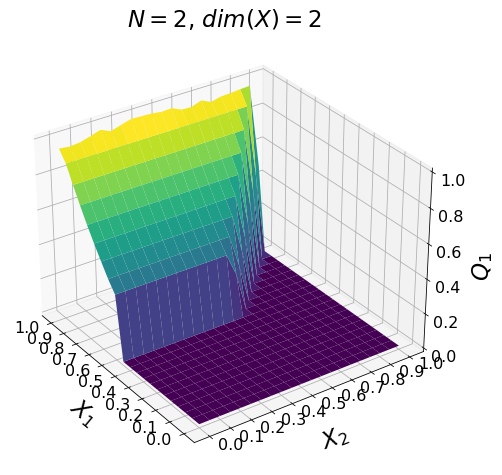
\includegraphics[width=0.6\textwidth]{images/symmetric_independent_unif_01_Q1.png}
        \end{center}
        
        \vspace{1mm}
        \raggedright{\small {\sc Figure \refstepcounter{fig}\thefig\label{fig:belloni_n2_q1}:} The interim allocation $Q_1$ for the first quality grade in the setting of symmetric, independent uniform setting of Pavlov \autocite*{pavlov2011optimal} when $X \sim U[0,1]^2$. Notice, for example, the allocation is monotonic in values of $X_1$ and that the reserve price $r \in [.5, .6)$.}
    \end{figure}

    \item Based on the description of the exclusive-buyer mechanism in Section \ref{subsec_ebm}, check if it matches the interim allocations yielded by the approximation algorithm. In Figure (\ref{fig:belloni_n2_q1}), the interim allocation from the approximation algorithm is compared to the interim allocation for the exclusive-buyer mechanism, given by: 
    \begin{equation}
        Q_1(x;r) = \mathbbm{1}\{ \beta_1 > \beta_2 \text{ and } \beta_1 \geq 0 \}F^{N-1}(x_1, \min\{\overline{x}_2, r_2 + \beta_1\})
    \end{equation}
    \noindent Examination of the interim allocations of mechanisms yielded by the approximation algorithms is the basis for hypotheses concerning the optimal mechanisms.
\end{enumerate}

\noindent By considering a wide enough range of cases and leveraging results from existing research in multidimensional mechanism design, we can develop some economic intuitions about the qualitative features of optimal mechanisms in a comparatively simpler multidimensional setting without worrying about the problem of bundling. Since this approach is broadly susceptible to problems of discretization when approximating the optimal mechanism as well as precision issues with numerical computing, conclusions are, at best, a promising guide to developing further theoretical results. Thus, results are best interpreted as conjectures concerning the character of optimal mechanisms in multidimensional settings.




\subsection{Conjectures}\label{subsec_conj}

The principal conjecture investigated in this thesis chapter concerns the optimality of the exclusive-buyer mechanism in the multidimensional setting of a single good with multiple quality levels:

\begin{conjecture}[Revenue]\label{conj_rev}
The revenue of the exclusive-buyer mechanism well-approximates the revenue of the optimal mechanism.
\end{conjecture}

\noindent By measuring the discrepancy between revenue from the exclusive-buyer mechanism and that returned by the approximation algorithm it is possible to confirm or reject this conjecture. 

It is also important to explore the interim allocations yielded by the approximation algorithm and compare them to those of the exclusive-buyer mechanism. There should be visual confirmation that the optimal mechanism yielded by the algorithm is qualitatively similar to the exclusive-buyer mechanism:

\begin{conjecture}[Allocations]\label{conj_alloc}
The allocation of the exclusive-buyer mechanism well-approximates the allocation of the optimal mechanism yielded by the approximation algorithm.
\end{conjecture}

\noindent Note, if Conjecture \ref{conj_alloc} holds, it automatically implies \ref{conj_rev}, since the allocations include the reserve price from which the revenue is calculated. However, since it is possible that the exclusive-buyer mechanism approximates the revenue of the optimal mechanism but fails to share qualitative features of its allocation, it is helpful to distinguish between both conjectures.

Additionally, a surprising feature of some optimal mechanisms in the setting of a single good with multiple quality levels noted by several economists is that the set of types excluded by the allocation in equilibrium---the \textit{exclusion region}---sometimes has measure zero (e.g., \cite{thirumulanathan2019, belloni2010multidimensional}). This surprising finding stands in opposition to the result of Armstrong \autocite*{armstrong1996multiproduct}, where it was shown that in the case of a multiproduct monopolist it is always optimal to exclude a positive measure of buyers. Thus, we explore under what circumstances the exclusion region is measure zero. Specifically, we conjecture:

\begin{conjecture}[Measure Zero Exclusion Region]\label{conj_excl_zero}
There exist multidimensional settings where a single good with multiple quality levels is sold to multiple bidders with a measure zero exclusion region.
\end{conjecture}

Finally, we conjecture that the exclusion region does not change with the number of bidders.

\begin{conjecture}[Same Exclusion Region for all $N$]\label{conj_excl_n}
The exclusion region of the optimal mechanism in the multidimensional setting of a single good with multiple quality levels remains the same for $N=1,2,3,\dots$ bidders. 
\end{conjecture}









\subsection{Simulations}\label{subsec_sim}

In what follows we explore the above conjectures in the following contexts:

\begin{enumerate}
    \item The \textbf{symmetric, independent, and uniform setting}, where buyers' valuations are independent across quality grades, uniformly and symmetrically distributed. I analyze the case where bidders have identical valuations for a good with two quality grades, where each valuation is assumed to be distributed $X_1,X_2 \sim U[0,1]$. Additionally, I analyze the case where $X_1,X_2 \sim U[2,3]$ since, in contrast to the previous setting, it is known that in these settings the optimal mechanism involves randomization when $N=1$. Analytic results in the single buyer case when $X \sim U[c,c+1]^2$ are known \autocite{pavlov2011optimal} and serve as a benchmark.

    \item The \textbf{symmetric, independent, and non-uniform setting}. Here, it is desirable to see if the conclusions reached in the first setting extend to non-uniform distributions. In particular, we consider the case of the $Beta(\alpha,\beta)$ distribution (where $\alpha=1,\beta=2$), which was explored in Daskalakis et al. \autocite*{daskalakis2017strong} in the context of multiple-goods.  

    \item The \textbf{symmetric, correlated setting}. It is unknown how arbitrary correlations between a buyer's valuations affect the revenue-maximization problem faced by the auction designer in multidimensional settings. This setting aims to shed light on this problem by considering buyers with valuations drawn from $X_1 = X_2 = [0,1]$ where the distribution of valuations is $f(x_1,x_2) = x_1 + x_2$.

    \item The \textbf{asymmetric, independent, and uniform setting}. No analytic results are known in this similar setting; however, a very provisional analysis of the optimality of the exclusive-buyer mechanism in this setting can be found in Belloni et al. \autocite*{belloni2010multidimensional}, where $X_1 \sim U[6,8], X_2 \sim U[9,11]$ with costs $c_1 = .9, c_2 = 5$. I replicate their analyses and extend their results in the context of the three conjectures proposed above.

    \item The \textbf{asymmetric, independent, and non-uniform setting}, a direct extension of the above setting where the valuations for each quality level of the good are drawn from two different truncated normal distributions. In particular, I consider the case where $X_1 \sim truncnorm(\mu=2.3, \sigma=1, \underline{x}_1=2, \overline{x}_1=3)$ and $X_2 \sim truncnorm(\mu=2.8, \sigma=.2, \underline{x}_2=2, \overline{x}_2=3)$.
\end{enumerate}




\subsubsection{Symmetric, independent, and uniform}

Analytic results in the case of a single buyer exist in the symmetric, independent, and uniform setting considered here. Pavlov \autocite*{pavlov2011optimal} studied the case of two substitute goods independently and uniformly distributed on $U[c,c+1]^2$. In the specific case of a single buyer with valuations distributed according to $X \sim U[0,1]^2$ with zero costs, it is known that the optimal mechanism is deterministic and involves setting reserve price $p^* =\frac{1}{\sqrt{3}}$ for both goods (since the valuations are symmetric). Thus, the optimal allocation is given in Figure \ref{fig:pavlov_alloc} and the auctioneer's revenue is simply $p^*( 1 - p^{*2} ) = 0.3849...$.
 
\begin{figure}[H]
    \begin{center}
    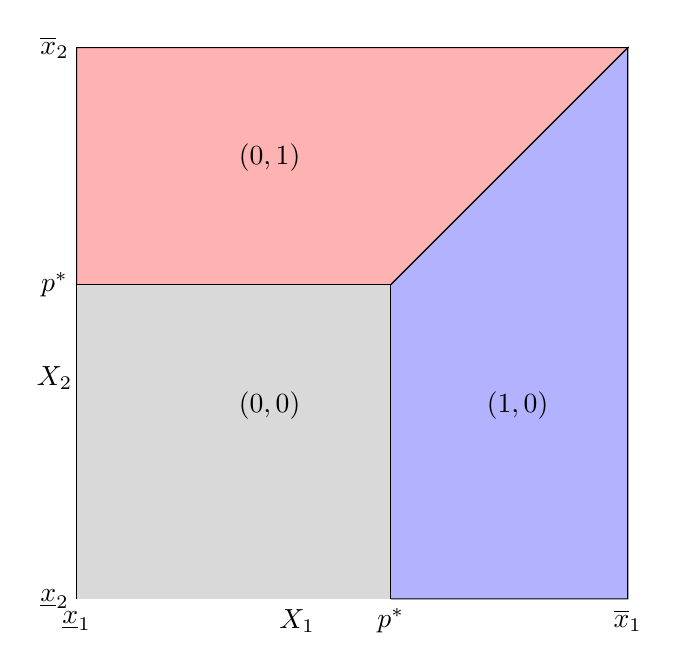
\begin{tikzpicture}[scale=.7]

    % square
    \draw (0,0) rectangle (10,10);

    % lines
    \draw (5.7,0) -- (5.7,5.7);
    \draw (0,5.7) -- (5.7,5.7);
    \draw (5.7,5.7) -- (10,10);

    % fill
    \draw[fill=red!30] (0,5.7) -- (0,10) -- (10,10) -- (5.7,5.7);
    \draw[fill=blue!30] (5.7,0) -- (10,0) -- (10,10) -- (5.7,5.7);
    \draw[fill=gray!30] (0,0) -- (0,5.7) -- (5.7,5.7) -- (5.7,0);

    % axis labels
    \node at (0,-.4) {$\underline{x}_1$};
    \node at (10,-.4) {$\overline{x}_1$};
    \node at (4,-.4) {$X_1$};
    \node at (5.7,-.4) {$p^*$};
    \node at (-.4,0) {$\underline{x}_2$};
    \node at (-.4,10) {$\overline{x}_2$};
    \node at (-.4,4) {$X_2$};
    \node at (-.4,5.7) {$p^*$};

    % region labels and lines
    \node at (3.5,3.5) {$(0,0)$};
    \node at (8,3.5) {$(1,0)$};
    \node at (3.5,8) {$(0,1)$};
    \end{tikzpicture}
    \end{center}
  
    \vspace{1mm}
    \raggedright{\small {\sc Figure \refstepcounter{fig}\thefig\label{fig:pavlov_alloc}:} The optimal allocation of a single good with two symmetric quality levels to a single buyer with valuations $X \sim U[0,1]^2$ \autocite{pavlov2011optimal}. The area denoted $(0,0)$ is the `exclusion region', where the good is not allocated. Note, in the setting of \autocite{pavlov2011optimal}, $p^*=\sqrt{1/3}$.}
\end{figure}

In the case where there is more than one bidder, we need to rely on the approximation algorithm to study the qualitative features of the optimal mechanism. First, we can confirm the approximation algorithm yields similar revenue to that calculated by the appropriate exclusive-buyer mechanism in this setting. These results are presented in Table \ref{table:pavlov_n2_revenue}.

\begin{center}
    \begin{tabular}{ |c|c|c| } 
    \hline
    Result Type & $T$ & Revenue \\
    \hline
    \hline
    approximation & 5 & 0.66094... \\ 
    approximation & 10 & 0.625929... \\ 
    approximation & 15 & 0.612877... \\ 
    approximation & 20 & 0.606033... \\ 
    exclusive-buyer mechanism & 50 & 0.589052... \\
    \hline
    \end{tabular}

    \vspace{1mm}
    \raggedright{\small {\sc Table \refstepcounter{fig}\thefig\label{table:pavlov_n2_revenue}:} The comparison of revenue generated by approximation algorithm with that of the exclusive-buyer mechanism. $T$ represents the number of intervals used to discretize each dimension of the buyers' valuations.}
\end{center}

\noindent Note that the revenue generated by the exclusive-buyer mechanism was computed using the \textit{ex-post} description of the auction. Additionally, the exclusive-buyer mechanism's revenue was computed by numerical integration on a finer discretization grid than that used by the approximation algorithm for increased precision. The trend for different $T$ implies that the approximation algorithm is converging to the result provided by the exclusive-buyer mechanism. This supports Conjecture \ref{conj_rev}. 

Using the interim allocation of the exclusive-buyer mechanism described in section \ref{subsec_ebm}, we can plot the allocations against those returned by the approximation algorithm. These are presented side-by-side in Figure \ref{fig:pavlov_n2_alloc}.

\begin{figure}[H]
    \begin{center}
    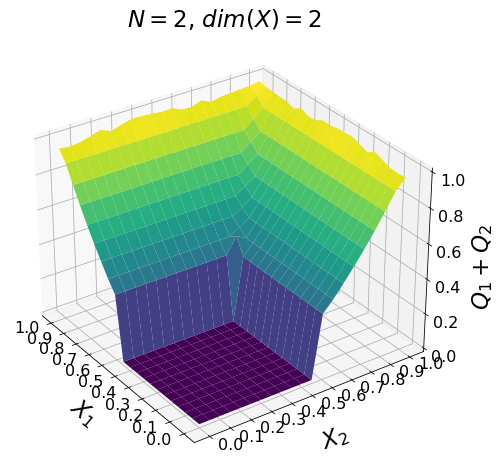
\includegraphics[width=0.45\textwidth]{images/symmetric_independent_unif_01.png}
    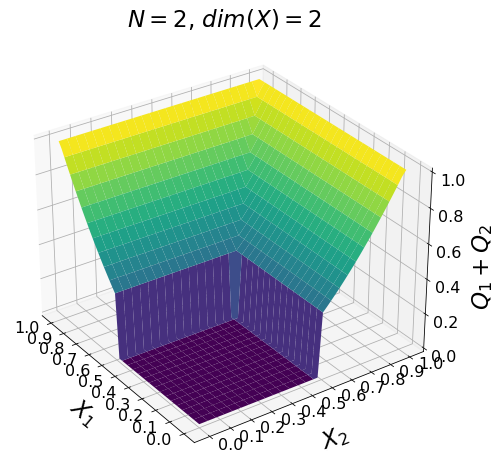
\includegraphics[width=0.44\textwidth]{images/symmetric_independent_unif_01_ebm.png}
    \end{center}
    
    \vspace{1mm}
    \raggedright{\small {\sc Figure \refstepcounter{fig}\thefig\label{fig:pavlov_n2_alloc}:} The allocations produced by the approximation algorithm (left) and exclusive-buyer mechanism (right).} 
\end{figure}

\noindent Conjecture \ref{conj_alloc} requires qualitatively evaluating the allocations returned from the approximation algorithm and those calculated from the exclusive-buyer mechanism, without an obvious means to conclusively determine whether the conjecture is supported. However, the results in Figure \ref{fig:pavlov_n2_alloc} imply that the exclusive-buyer mechanism captures the behavior of the (approximately) optimal mechanism. Thus, these results offer support for Conjecture \ref{conj_alloc}.

Notice that the exclusion region in Figure \ref{fig:pavlov_n2_alloc} is similar to that discovered in Pavlov \autocite*{pavlov2011optimal}. This is evidence against Conjecture \ref{conj_excl_zero} concerning the existence of measure zero exclusion regions. The price $p^* = \frac{1}{\sqrt{3}} = 0.577...$ that maximizes revenue in the case when $N=1$ is consistent with the exclusion region defined by $p^* = 0.6$ returned by the approximation algorithm for the case of $N=2$. (Note that when $[0,1]$ is discretized into 20 intervals, the price is $p \in \{\dots, .5, .55, .6, \dots\}$ so the choice by the algorithm reflects its approximate optimality). Indeed, when $T=20$, the approximation algorithm yields the same exclusion region for all of $N=1,2,3$. This supports Conjecture \ref{conj_excl_n}.

% \begin{figure}[H]
%     \begin{center}
%     \begin{tikzpicture}[scale=.7]
%     % square
%     \draw (0,0) rectangle (10,10);

%     % lines
%     \draw (5.77,0) -- (5.77,5.77);
%     \draw (0,5.77) -- (5.77,5.77);
%     \draw (5.77,5.77) -- (10,10);

%     % fill
%     \draw[fill=gray!30] (0,0) -- (0,5.77) -- (5.77,5.77) -- (5.77,0);

%     % axis labels
%     \node at (0,-.4) {$\underline{x}_1$};
%     \node at (10,-.4) {$\overline{x}_1$};
%     \node at (4,-.4) {$X_1$};
%     \node at (5.77,-.4) {$p^*$};
%     \node at (-.4,0) {$\underline{x}_2$};
%     \node at (-.4,10) {$\overline{x}_2$};
%     \node at (-.4,4) {$X_2$};
%     \node at (-.4,5.77) {$p^*$};

%     % region labels and lines
%     \node at (3.5,3.5) {$(0,0)$};

%     \end{tikzpicture}
%     \end{center}
  
%     \vspace{1mm}
%     \raggedright{\small {\sc Figure \refstepcounter{fig}\thefig\label{fig:pavlov_all_n_excl}:} The exclusion region produced by the approximation algorithm when $T=20$ for each of $N=1,2,3$. As noted above, due to the discretization $T=20$, $p^* = 0.6$.}
% \end{figure}

Furthermore, it is helpful to investigate the behavior of the approximation algorithm when $X \sim U[2,3]^2$, since we know from Pavlov \autocite*{pavlov2011optimal} that the optimal mechanism is stochastic. This is particularly important in the context of Conjecture \ref{conj_excl_n} since it implies that the exclusive-buyer mechanism will not be optimal in this case.

Again, first, we confirm the approximation algorithm yields similar revenue to that calculated by the appropriate exclusive-buyer mechanism in this setting. These results are presented in Table \ref{table:pavlov_23_n2_revenue}.

\begin{center}
    \begin{tabular}{ |c|c|c| } 
    \hline
    Result Type & $T$ & Revenue \\
    \hline
    \hline
    approximation & 5 & 2.622409... \\ 
    approximation & 10 & 2.58287... \\ 
    approximation & 15 & 2.58287... \\ 
    approximation & 20 & 2.562314... \\ 
    exclusive-buyer mechanism & 50 & 2.534499... \\
    \hline
    \end{tabular}

    \vspace{1mm}
    \raggedright{\small {\sc Table \refstepcounter{fig}\thefig\label{table:pavlov_23_n2_revenue}:} The comparison of revenue generated by approximation algorithm with that of the exclusive-buyer mechanism. Since the mechanism yielded by the approximation algorithm included randomization and, therefore, the menu of contract points included more than a single reserve price, the choice of reserve price for the exclusive-buyer mechanism was $r=2.15$.}
\end{center}

\noindent Here, the exclusive-buyer mechanism yields a revenue similar to that of the optimal mechanism. The difference between the revenues is approximately 1\%, despite the stochastic optimal mechanism. Furthermore, there is a clear indication that as $T$ increases, the approximation algorithm converges to the revenue yielded by the exclusive-buyer mechanism. This supports Conjecture \ref{conj_rev}.

We can plot the allocations of the optimal mechanism generated by the approximation algorithm with those of the exclusive-buyer mechanism to assess our next conjecture. These are presented side-by-side in Figure \ref{fig:pavlov_n2_23_alloc}.

\begin{figure}[H]
    \begin{center}
    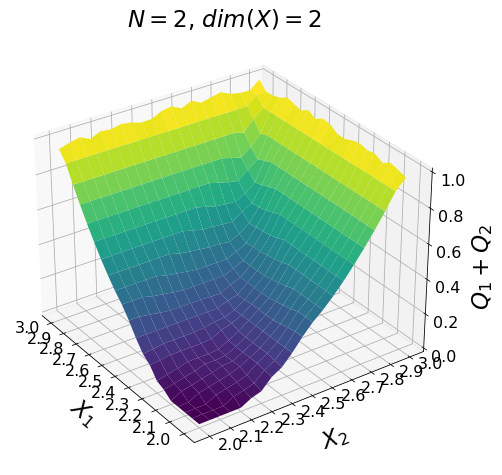
\includegraphics[width=0.45\textwidth]{images/symmetric_independent_unif_23.png}
    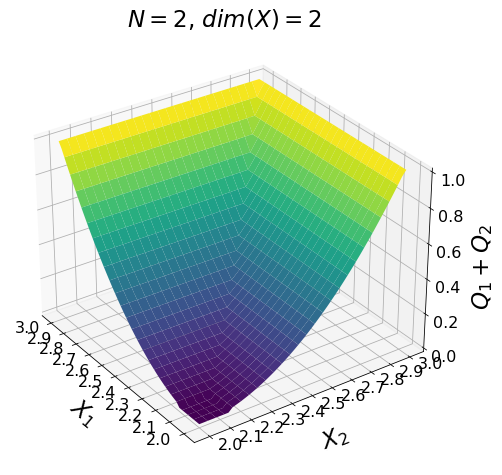
\includegraphics[width=0.44\textwidth]{images/symmetric_independent_unif_23_ebm.png}
    \end{center}
    
    \vspace{1mm}
    \raggedright{\small {\sc Figure \refstepcounter{fig}\thefig\label{fig:pavlov_n2_23_alloc}:} The allocations produced by the approximation algorithm (left) and exclusive-buyer mechanism (right).} 
\end{figure}

\noindent Although the shape of the allocations is similar in the region where $Q_1(x) + Q_2(x) > 0$, the exclusion region yielded by the optimal mechanism is triangular, indicating that the optimal mechanism includes randomization. In contrast, the exclusive-buyer mechanism is a deterministic mechanism and has a rectangular exclusion region. Thus, this setting does not support Conjecture \ref{conj_alloc}.

Again, the exclusion region in Figure \ref{fig:pavlov_n2_23_alloc} is similar to that discovered in Pavlov \autocite*{pavlov2011optimal}. This is notable because when $X \sim [c,c+1]^2$ there was randomization in the single bidder case. This is both evidence against Conjecture \ref{conj_excl_zero} concerning the existence of measure zero exclusion regions and evidence for Conjecture \ref{conj_excl_n}. Indeed, when $T=20$, the approximation algorithm yields the same exclusion region for all of $N=1,2,3$.





\subsubsection{Symmetric, independent, and non-uniform setting}

I examine the four conjectures in the context of a symmetric, independent, and non-uniform setting. Following the multi-unit example in Daskalakis et al. \autocite*{daskalakis2017strong}, I consider the case where $X_1,X_2 \sim Beta(\alpha,\beta)$ where $\alpha=1,\beta=2$. To the best of my knowledge, no prior work on analytic solutions to the optimal auction design problem exists in this setting. Therefore, we proceed by running the optimization algorithm and comparing the output of the algorithm to that provided by the exclusive-buyer mechanism described above.

First, we compare the revenue generated by the approximation algorithm and the exclusive-buyer mechanism. The results are presented in Table \ref{table:symm_beta_revenue}. Again, note the revenue from the exclusive-buyer mechanism was calculated using \textit{ex-post} allocations from a second-price auction. Although the revenue generated from the optimal mechanism is larger than the exclusive-buyer mechanism ($\sim$4\%), the trend as $T$ increases provides support for Conjecture \ref{conj_rev}.

\begin{center}
    \begin{tabular}{ |c|c|c| } 
    \hline
    Result Type & $T$ & Revenue \\
    \hline
    \hline
    approximation & 5 & 0.448709... \\ 
    approximation & 10 & 0.418815... \\ 
    approximation & 15 & 0.406948... \\ 
    approximation & 20 & 0.400615... \\ 
    exclusive-buyer mechanism & 50 & 0.385045... \\
    \hline
    \end{tabular}

    \vspace{1mm}
    \raggedright{\small {\sc Table \refstepcounter{fig}\thefig\label{table:symm_beta_revenue}:} The comparison of revenue generated by the approximation algorithm with that of the exclusive-buyer mechanism when $X_1,X_2 \sim Beta(1,2)$.}
\end{center}

Next, we can compare the interim allocations from the approximation algorithm with those from the exclusive-buyer mechanism. These are displayed graphically in Figure \ref{fig:beta12_alloc}. There is a clear similarity between both allocations, supporting Conjecture \ref{conj_alloc}.

\begin{figure}[H]
    \begin{center}
    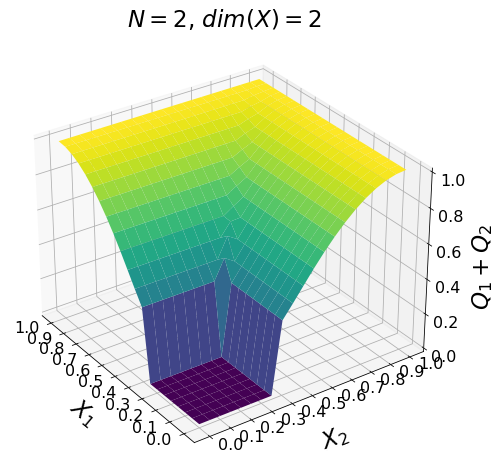
\includegraphics[width=0.45\textwidth]{images/symmetric_independent_beta.png}
    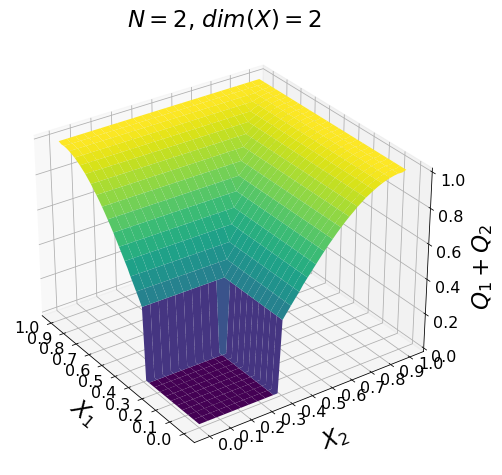
\includegraphics[width=0.44\textwidth]{images/symmetric_independent_beta_ebm.png}
    \end{center}
    
    \vspace{1mm}
    \raggedright{\small {\sc Figure \refstepcounter{fig}\thefig\label{fig:beta12_alloc}:} The allocations produced by the approximation algorithm (left) and exclusive-buyer mechanism (right).} 
\end{figure}


\noindent Note, these allocations offer a lack of support of Conjecture \ref{conj_excl_zero} concerning the existence of measure zero exclusion regions.

Finally, running the approximation algorithm for $N=1,2,3$ confirms Conjecture \ref{conj_excl_n}. The exclusion region is the same for all $N$ tested: the value of $p^*=0.4$. (Recall, discretization of the grid into $T=20$ intervals per quality level requires that $p^* \in \{\dots, 0.35, 0.4, 0.45, \dots\}$).  

% \begin{figure}[H]
%     \begin{center}
%     \begin{tikzpicture}[scale=.7]
%     % square
%     \draw (0,0) rectangle (10,10);

%     % lines
%     \draw (4,0) -- (4,4);
%     \draw (0,4) -- (4,4);

%     % fill
%     \draw[fill=gray!30] (0,0) -- (0,4) -- (4,4) -- (4,0);

%     % axis labels
%     \node at (0,-.4) {$\underline{x}_1$};
%     \node at (10,-.4) {$\overline{x}_1$};
%     \node at (4,-.4) {$p^*$};
%     \node at (6,-.4) {$X_1$};
%     \node at (-.4,0) {$\underline{x}_2$};
%     \node at (-.4,10) {$\overline{x}_2$};
%     \node at (-.4,4) {$p^*$};
%     \node at (-.4,6) {$X_2$};

%     % region labels and lines
%     \node at (2,2) {$(0,0)$};
%     \end{tikzpicture}
%     \end{center}
  
%     \vspace{1mm}
%     \raggedright{\small {\sc Figure \refstepcounter{fig}\thefig\label{fig:beta12_all_n_excl}:} The exclusion region produced by the approximation algorithm when $T=20$ for each of $N=1,2,3$. Note, in this setting, $p^*=0.4$.}
% \end{figure}

Thus, in conclusion, all conjectures are supported in the setting of symmetric, independent, and non-uniform distributions except for Conjecture \ref{conj_excl_zero} concerning the existence of a measure zero exclusion region.







\subsubsection{Symmetric, correlated setting}

In this setting, I allow for the valuations $X_1$ and $X_2$ to be correlated. Here, $X_1 = X_2 = [0,1]$, where $X \sim F$ and $f(x_1,x_2) = x_1+x_2$. This extension of the previous settings on the unit square facilitates a deeper understanding of correlated valuations in a familiar setting. As above, I proceed by running the approximation algorithm and comparing the results with those from the exclusive-buyer mechanism.

With regard to revenue, we can see in Table \ref{table:symm_correlated_revenue} that the algorithm's revenue is, again, well-approximated by the exclusive-buyer mechanism ($\sim$3\%). The trend as $T$ increases is similar to the other settings: the revenue generated by the approximation algorithm converges to that yielded by the exclusive-buyer mechanism. This supports Conjecture \ref{conj_rev}.

\begin{center}
    \begin{tabular}{ |c|c|c| } 
    \hline
    Result Type & $T$ & Revenue \\
    \hline
    \hline
    approximation & 5 & 0.75159... \\ 
    approximation & 10 & 0.718683... \\ 
    approximation & 15 & 0.705905... \\ 
    approximation & 20 & 0.698962... \\ 
    exclusive-buyer mechanism & 50 & 0.676192... \\
    \hline
    \end{tabular}

    \vspace{1mm}
    \raggedright{\small {\sc Table \refstepcounter{fig}\thefig\label{table:symm_correlated_revenue}:} The comparison of revenue generated by the approximation algorithm with that of the exclusive-buyer mechanism when $f(x_1,x_2) = x_1 + x_2$.}
\end{center}

The allocations are also similar. The interim allocations from the approximation algorithm and the exclusive-buyer mechanism are presented in Figure \ref{fig:symmetric_correlated_alloc}. This supports Conjecture \ref{conj_alloc} concerning the qualitative similarity of the optimal mechanism yielded by the approximation algorithm and that of the exclusive-buyer mechanism.

\begin{figure}[H]
    \begin{center}
    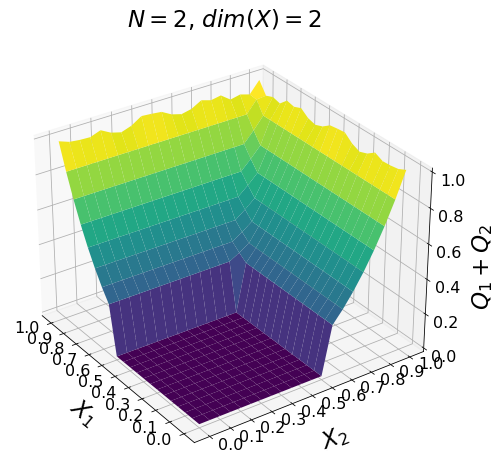
\includegraphics[width=0.45\textwidth]{images/symmetric_correlated_unif.png}
    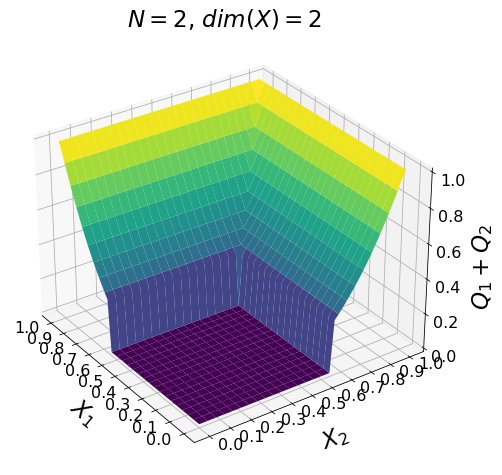
\includegraphics[width=0.44\textwidth]{images/symmetric_correlated_unif_ebm.png}
    \end{center}
    
    \vspace{1mm}
    \raggedright{\small {\sc Figure \refstepcounter{fig}\thefig\label{fig:symmetric_correlated_alloc}:} The allocations produced by the approximation algorithm (left) and the exclusive-buyer mechanism (right).} 
\end{figure}

\noindent Again, note the presence of an exclusion region undermines support for Conjecture \ref{conj_excl_zero} concerning the existence of settings without an exclusion region.

Finally, the exclusion regions in the symmetric, correlated, uniform setting where $X_1 = X_2 = [0,1]$ and $f(x_1,x_2) = x_1 + x_2$ are the same for all $N=1,2,3$. Note, the reserve price is $p^* = .65$ in this setting. This supports Conjecture \ref{conj_excl_n}.

% \begin{figure}[H]
%     \begin{center}
%     \begin{tikzpicture}[scale=.7]
%     % square
%     \draw (0,0) rectangle (10,10);

%     % lines
%     \draw (6.5,0) -- (6.5,6.5);
%     \draw (0,6.5) -- (6.5,6.5);

%     % fill
%     \draw[fill=gray!30] (0,0) -- (0,6.5) -- (6.5,6.5) -- (6.5,0);

%     % axis labels
%     \node at (0,-.4) {$\underline{x}_1$};
%     \node at (10,-.4) {$\overline{x}_1$};
%     \node at (6.5,-.4) {$p^*$};
%     \node at (4,-.4) {$X_1$};
%     \node at (-.4,0) {$\underline{x}_2$};
%     \node at (-.4,10) {$\overline{x}_2$};
%     \node at (-.4,6.5) {$p^*$};
%     \node at (-.4,4) {$X_2$};

%     % region labels and lines
%     \node at (3.5,3.5) {$(0,0)$};
%     \end{tikzpicture}
%     \end{center}
  
%     \vspace{1mm}
%     \raggedright{\small {\sc Figure \refstepcounter{fig}\thefig\label{fig:symm_correlated_all_n_excl}:} The exclusion region produced by the approximation algorithm when $T=20$ for each of $N=1,2,3$. Note, in this setting, $p^*=.65$.}
% \end{figure}

As in the previous setting, all conjectures except for Conjecture \ref{conj_excl_zero} concerning the existence of a measure zero exclusion region are supported.








\subsubsection{Asymmetric, independent, and uniform setting}

In this setting, we consider the case where $X_1 \sim U[6,8]$ and $X_2 \sim U[9,11]$ as considered in \autocite{belloni2010multidimensional}, who first studied the optimality of the exclusive-buyer mechanism in multidimensional settings. Additionally, the costs associated with selling the first quality grade of the good are $c_1 = .9$ and the second quality grade are $c_2 = 5$. Since prior computational work exists assessing the optimality of the exclusive-buyer mechanism, where possible, I can compare my findings here with those in Belloni et al. \autocite*{belloni2010multidimensional}. 

The revenue yielded by the approximation algorithm is similar to that of the exclusive-buyer mechanism. The data are displayed in Table \ref{table:asymm_belloni}. These revenue numbers are consistent with those in \autocite[Table 3]{belloni2010multidimensional}, supporting Conjecture \ref{conj_rev}, namely, that the revenue of the optimal mechanism is well-approximated by the exclusive-buyer mechanism.

\begin{center}
    \begin{tabular}{ |c|c|c| } 
    \hline
    Result Type & $T$ & Revenue \\
    \hline
    \hline
    approximation & 5 & 6.02496... \\ 
    approximation & 10 & 5.941549... \\ 
    approximation & 15 & 5.91222... \\ 
    approximation & 20 & 5.893113... \\ 
    exclusive-buyer mechanism & 50 & 5.805032... \\
    \hline
    \end{tabular}

    \vspace{1mm}
    \raggedright{\small {\sc Table \refstepcounter{fig}\thefig\label{table:asymm_belloni}:} The comparison of revenue generated by the approximation algorithm with that of the exclusive-buyer mechanism in the setting of Belloni et al. \autocite*{belloni2010multidimensional}.}
\end{center}

With regard to the allocations, we can see a clear disparity between the interim allocations produced by the approximation algorithm and those of the exclusive-buyer mechanism. The exclusive-buyer mechanism's interim allocation for $Q_1(x) + Q_2(x)$ is much lower for large values of $X_2$ than that of the approximation algorithm. The allocations are presented in Figure \ref{fig:belloni_alloc}.

\begin{figure}[H]
    \begin{center}
    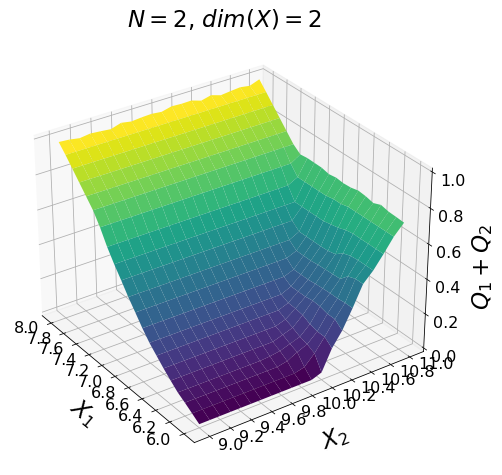
\includegraphics[width=0.45\textwidth]{images/asymmetric_independent_belloni.png}
    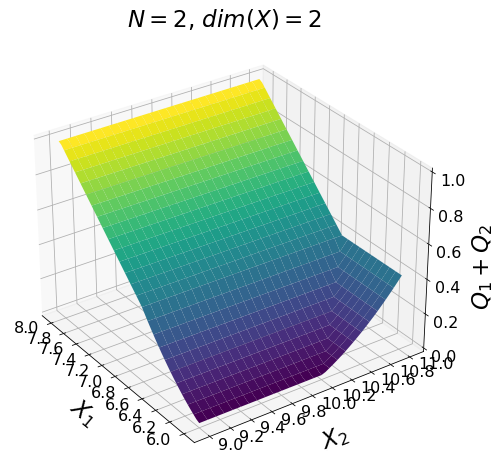
\includegraphics[width=0.44\textwidth]{images/asymmetric_independent_belloni_ebm.png}
    \end{center}
    
    \vspace{1mm}
    \raggedright{\small {\sc Figure \refstepcounter{fig}\thefig\label{fig:belloni_alloc}:} The allocations produced by the approximation algorithm (left) and the exclusive-buyer mechanism (right).} 
\end{figure}

\noindent This surprising feature of the exclusive-buyer mechanism's interim allocation suggests that Conjecture \ref{conj_alloc} is \textit{not} supported in the asymmetric, independent, and uniform setting. Here, although the optimal revenue is well approximated by the exclusive-buyer mechanism, the qualitative features of the optimal mechanism are sufficiently different from those conjectured by the exclusive-buyer mechanism. I explore this result in more detail in the discussion section \ref{sec_discuss} below.

Notice, however, in this setting Conjecture \ref{conj_excl_zero} is supported. This is visible in Figure \ref{fig:belloni_alloc_alln} below. This was also noted in the simulations of Belloni et al. \autocite*{belloni2010multidimensional}, suggesting it is robust to computational or approximation error. Additionally, Conjecture \ref{conj_excl_n} is supported for all $N=1,2,3$; however, it is important to note a number of surprising features of the optimal mechanism yielded by the approximation algorithm in this setting. Firstly, although the exclusion region is the same for all $N$, the allocation itself varies with the number of buyers. Secondly, there is evidence of randomization in the optimal mechanism yielded by the approximation algorithm. 

\begin{figure}[H]
    \begin{center}
    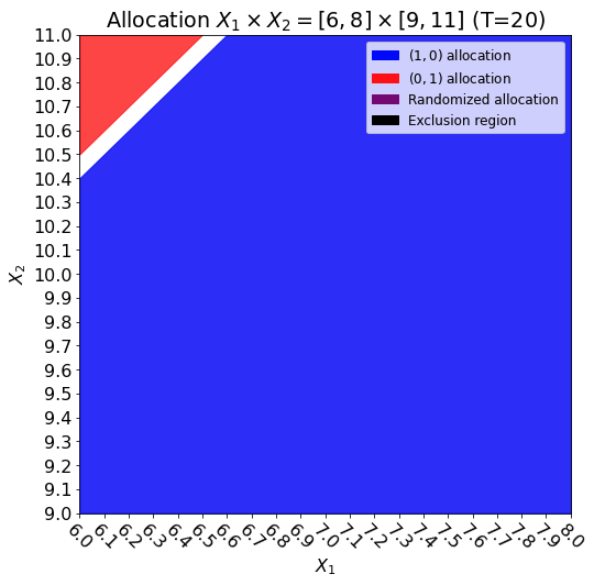
\includegraphics[width=0.45\textwidth]{images/belloni_alloc_n1.png}
    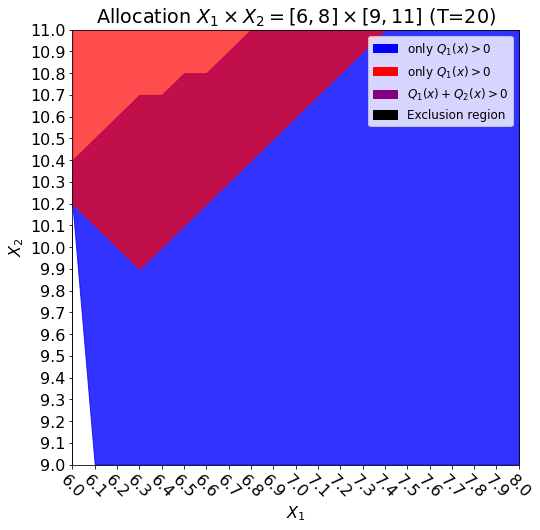
\includegraphics[width=0.44\textwidth]{images/belloni_alloc_n2.png}
    \end{center}
    
    \vspace{1mm}
    \raggedright{\small {\sc Figure \refstepcounter{fig}\thefig\label{fig:belloni_alloc_alln}:} Graphs showing where the allocations for the first ($Q_1$) and second ($Q_2$) quality level of the good are non-zero for the optimal mechanism yielded by the approximation algorithm for $N=1$ (left) and $N=2$ (right).} 
\end{figure}

Thus, in the symmetric correlated setting, although Conjectures \ref{conj_rev}, \ref{conj_excl_zero}, \ref{conj_excl_n} are supported, Conjecture \ref{conj_alloc} is not. The complexities of this result will be further explored below.







\subsubsection{Asymmetric, independent, and non-uniform setting}

I extend the investigation of asymmetric settings by considering the cases where buyers' valuations are distributed according to two different distributions. In particular, I consider the case where the valuations are drawn from $X_1 = X_2 = [2,3]$ and the distribution of valuations is asymmetric, where $X_1 \sim truncnorm(\mu=2.3, \sigma=1)$ and $X_2 \sim truncnorm(\mu=2.8, \sigma=.2)$. Note, in contrast to the previous asymmetric setting considered above, in this setting the sets from which the valuations are drawn are equal (i.e., $X_1 = X_2$) but the distributions are not (i.e., $f_1(x) \neq f_2(x)$). Again, no prior analytic results exist in this setting and therefore I proceed by running the approximation algorithm for the optimal auction and comparing the result to that of the exclusive-buyer mechanism.

First, I compare the revenue generated by the approximation algorithm and the exclusive-buyer mechanism. This is presented in Table \ref{table:asymm_truncnorm_revenue}. The similarity of the revenues generated by the approximation algorithm and the exclusive-buyer mechanism lends support to Conjecture \ref{conj_rev}.

\begin{center}
    \begin{tabular}{ |c|c|c| } 
    \hline
    Result Type & $T$ & Revenue \\
    \hline
    \hline
    approximation & 5 & 2.779996... \\ 
    approximation & 10 & 2.749451... \\ 
    approximation & 15 & 2.736171... \\ 
    approximation & 20 & 2.729342... \\ 
    exclusive-buyer mechanism & 50 & 2.57921... \\
    \hline
    \end{tabular}

    \vspace{1mm}
    \raggedright{\small {\sc Table \refstepcounter{fig}\thefig\label{table:asymm_truncnorm_revenue}:} The comparison of revenue generated by the approximation algorithm with that of the exclusive-buyer mechanism when $X_1 \sim truncnorm(\mu=2.3, \sigma=1, \underline{x}_1=2, \overline{x}_1=3)$ and $X_2 \sim truncnorm(\mu=2.8, \sigma=.2, \underline{x}_2=2, \overline{x}_2=3)$.}
\end{center}

When we compare the interim allocations generated by the approximation algorithm to those of the exclusive-buyer mechanism in Figure \ref{fig:truncnorm_alloc}, we can qualitatively see that the allocations are similar. This supports Conjecture \ref{conj_alloc}.

\begin{figure}[H]
    \begin{center}
    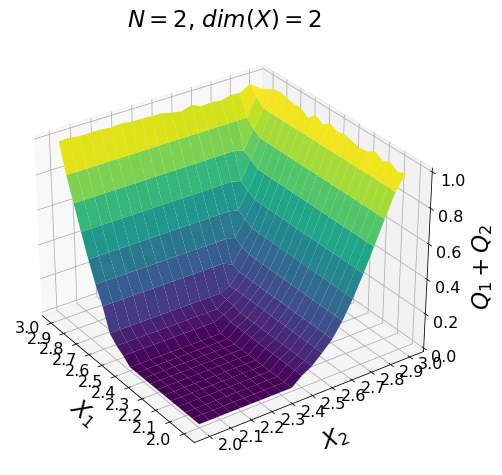
\includegraphics[width=0.45\textwidth]{images/asymmetric_independent_truncnorm.png}
    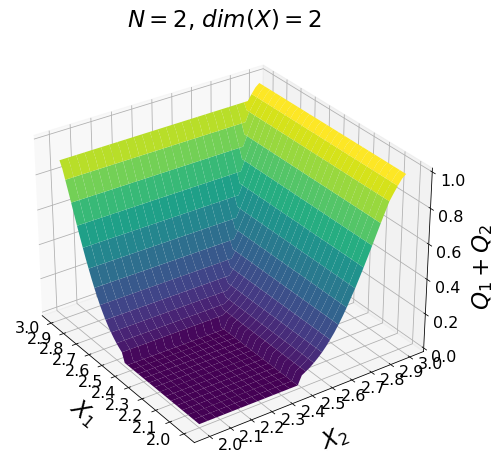
\includegraphics[width=0.44\textwidth]{images/asymmetric_independent_truncnorm_ebm.png}
    \end{center}
    
    \vspace{1mm}
    \raggedright{\small {\sc Figure \refstepcounter{fig}\thefig\label{fig:truncnorm_alloc}:} The allocations produced by the approximation algorithm (left) and exclusive-buyer mechanism (right).} 
\end{figure}

\noindent Additionally, note that the existence of an exclusion region in Figure \ref{fig:truncnorm_alloc} above undermines Conjecture \ref{conj_excl_zero}.

Finally, running the approximation algorithm for all $N=1,2,3$ confirms Conjecture \ref{conj_excl_n}. In this asymmetric setting $p_1^* = 2.55$ and $p_2^* = 2.5$ and the exclusion region remains the same for all $N$. 

% \begin{figure}[H]
%     \begin{center}
%     \begin{tikzpicture}[scale=.7]
%     % square
%     \draw (0,0) rectangle (10,10);

%     % lines
%     \draw (5.5,0) -- (5.5,5);
%     \draw (0,5) -- (5.5,5);

%     % fill
%     \draw[fill=gray!30] (0,0) -- (5.5,0) -- (5.5,5) -- (0,5);

%     % axis labels
%     \node at (0,-.4) {$\underline{x}_1$};
%     \node at (10,-.4) {$\overline{x}_1$};
%     \node at (5.5,-.4) {$p_1^*$};
%     \node at (4,-.4) {$X_1$};
%     \node at (-.4,0) {$\underline{x}_2$};
%     \node at (-.4,10) {$\overline{x}_2$};
%     \node at (-.4,5) {$p_2^*$};
%     \node at (-.4,4) {$X_2$};

%     % region labels and lines
%     \node at (2,2) {$(0,0)$};
%     \end{tikzpicture}
%     \end{center}
  
%     \vspace{1mm}
%     \raggedright{\small {\sc Figure \refstepcounter{fig}\thefig\label{fig:truncnorm_all_n_excl}:} The exclusion region produced by the approximation algorithm when $T=20$ for each of $N=1,2,3$. Note, in this setting, $p_1^*=2.55, p_2^*=2.5$.}
% \end{figure}

Thus, in conclusion, all conjectures except for Conjecture \ref{conj_excl_zero} concerning the existence of a measure zero exclusion region are supported in the setting of asymmetric, independent, and non-uniform distributions.




\section{Discussion \& Conclusion}\label{sec_discuss}

Analytic results concerning the qualitative characteristics of optimal auctions in multidimensional settings are scarce. In this chapter, I explored the particular multidimensional setting of a single good with multiple quality levels. In particular, I investigated whether the exclusive-buyer mechanism is optimal in this setting. To do this, I developed an approximation algorithm that facilitates the investigation of the optimal mechanism in multidimensional settings and compared the performance of the exclusive-buyer mechanism to that of the optimal mechanism yielded by the approximation algorithm. 

I explored four conjectures concerning the optimality of the exclusive-buyer mechanism in the multidimensional setting of a single good with multiple quality levels. The rest of this section contains a discussion of how the results presented in Section \ref{subsec_sim} support or undermine these conjectures.

\subsection{Conjecture \ref{conj_rev} (Revenue)}

This conjecture asserted that ``the revenue of the exclusive-buyer mechanism well-approximates the revenue of the optimal mechanism''. Across all settings considered above, this conjecture is supported. However, support for this conjecture alone is far from sufficient to demonstrate the optimality of the exclusive-buyer mechanism. It is well known that simple (deterministic) mechanisms can approximate optimal (stochastic) mechanisms up to some constant fraction of their revenue. This approximation can often be very close to the revenue yielded by the optimal mechanism. In the case where a single bidder's valuations are uniformly distributed on the unit square $X \sim [c,c+1]^2$, the gain from using a fully optimal mechanism over the best deterministic mechanism is at most 1.2\% \autocite[p11]{pavlov2011optimal}. Though in some settings considered here with $N=2$ bidders, the gain is closer to 3-4\%, the trend as $T$ increases suggests that the final gain from using optimal mechanism over the exclusive-buyer mechanism is closer to $\sim$1-2\% in instances where randomization is required for optimality. Furthermore, the results are also consistent with previous simulation studies on the optimality of the exclusive-buyer mechanism indicating it well-approximates the revenue generated by the optimal mechanism \autocite{belloni2010multidimensional}. Thus, the results support Conjecture \ref{conj_rev}.

\subsection{Conjecture \ref{conj_alloc} (Allocations)}

Across all settings considered here, the interim allocations of the optimal mechanism yielded by the approximation algorithm share qualitative features with the exclusive-buyer mechanism's allocations. However, there are multiple cases where the allocations are noticeably different. Thus, there is mixed support for Conjecture \ref{conj_alloc}, which asserts that ``the allocation of the exclusive-buyer mechanism well-approximates the allocation of the optimal mechanism yielded by the approximation algorithm.'' I consider each of these cases in turn.

There is evidence of support for Conjecture \ref{conj_alloc} in the following settings:
\begin{itemize}
    \item Symmetric, independent, and uniform setting ($X \sim U[0,1]^2$)
    \item Symmetric, independent, and non-uniform setting ($X \sim Beta(1,2)^2$)
    \item Symmetric, correlated, and uniform setting ($X \sim F, f(x_1,x_2) = x_1 + x_2$)
    \item Asymmetric, independent, and non-uniform setting ($X_1 \sim truncnorm(\mu=2.3, \sigma=1, \underline{x}_1=2, \overline{x}_1=3)$, $X_2 \sim truncnorm(\mu=2.8, \sigma=.2, \underline{x}_2=2, \overline{x}_2=3)$)
\end{itemize}
\noindent In each of these settings, the reserve prices were consistent and the allocations were qualitatively similar in the region where $Q_1(x) + Q_2(x) > 0$. It is noteworthy that in each of these settings, the optimal mechanism is deterministic. 

There is evidence against Conjecture \ref{conj_alloc} in the symmetric, independent, and uniform setting ($X \sim U[2,3]^2$) and the asymmetric, independent, and uniform setting first investigated by Belloni et al. \autocite*{belloni2010multidimensional}. In both these settings there is evidence of randomization in the optimal mechanism, which suggests the deterministic exclusive-buyer mechanism is unable to approximate the optimal allocations. In the former case when $X \sim U[2,3]^2$ the exclusion region is not rectangular. In the latter case, the exclusion region has measure zero and, on closer inspection, evidence of randomization can be seen in Figure \ref{fig:belloni_alloc_Q1} where the allocations for each quality grade are shown separately. As can be seen in the graph of $Q_1$ on the left, a `fold' in the allocation occurs around the line $x_1 - c_1 = x_2 - c_2$ (recall, $c_1=.9, c_2=5$). In this region, both $Q_1(x) > 0$ and $Q_2(x) > 0$.


\begin{figure}[H]
    \begin{center}
    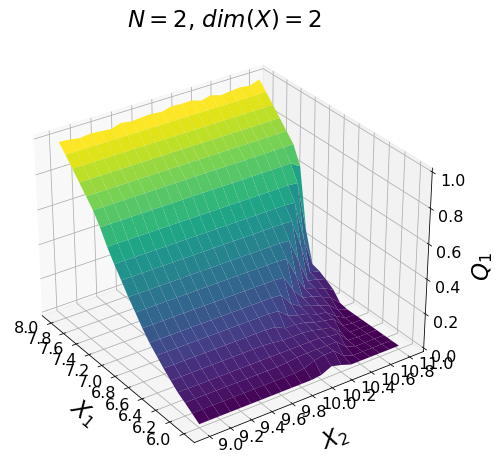
\includegraphics[width=0.45\textwidth]{images/asymmetric_independent_belloni_Q1.png}
    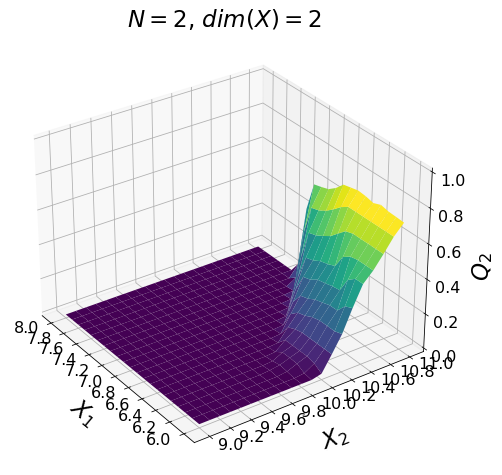
\includegraphics[width=0.45\textwidth]{images/asymmetric_independent_belloni_Q2.png}
    \end{center}
    
    \vspace{1mm}
    \raggedright{\small {\sc Figure \refstepcounter{fig}\thefig\label{fig:belloni_alloc_Q1}:} The allocation $Q_1$ for the first quality level (left) and $Q_2$ for the second quality level (right) of the good produced by the approximation algorithm when $N=2$.} 
\end{figure}

In conclusion, there is mixed support for Conjecture \ref{conj_alloc}. When the optimal mechanism exhibits randomization, the allocations of the deterministic exclusive-buyer mechanism do not well-approximate optimal allocations. However, it is possible to construct an \textit{stochastic exclusive-buyer mechanism} which includes lotteries. The idea is simple: again, each bidder bids to be the only bidder to choose between quality grades of the object. They can then purchase one of any number of lotteries determined by the seller. This mechanism was not considered in this chapter but future work should address whether it might be optimal in the multidimensional setting of a single good with multiple quality grades.





\subsection{Conjecture \ref{conj_excl_zero} (Measure Zero Exclusion Region)}

Conjecture \ref{conj_excl_zero} concerns the existence of ``multidimensional settings where a single good with multiple quality levels is sold to multiple bidders with a measure zero exclusion region''. Only the asymmetric, independent, and uniform setting initially investigated by Belloni et al. \autocite*{belloni2010multidimensional} provides evidence for this conjecture. This finding was also discussed in the work of Thirumulanathan et al. \autocite*{thirumulanathan2019unitdemand}, who studied the multidimensional setting of a single good with multiple quality levels when bidder valuations are uniformly distributed on an arbitrary rectangle $[a,b] \times [c,d]$. 

This finding stands in contrast to theoretical work in multidimensional mechanism design where it has been shown in the multi-unit case that it is always optimal to exclude a positive measure of bidder types \autocite{armstrong1996multiproduct,rochet1998ironing}. Notice that in the example considered above the typespace $[6,8]\times[9,11]$ violates the assumption of strict convexity. This assumption is essential to establish Armstrong's \autocite*{armstrong1996multiproduct} proof. In the case of Rochet and Choné \autocite*{rochet1998ironing}, they require the cost function to be smooth, which is clearly violated in the setting above.

Figure \ref{fig:belloni_alloc} suggests that for the mechanism yielded by the approximation algorithm, there is an interval $6\times [9,p^*]$ for some $p^*\in [9,11]$ that receives zero utility in equilibrium. The measure of this interval is zero. However, contrary to \autocite[Proposition 1]{armstrong1996multiproduct}, if one increases the price by $\epsilon$, one would exclude a mass of types proportional to $\epsilon$ and not $\epsilon^2$. This intuition suggests why optimal mechanisms might be characterized by measure zero exclusion regions in asymmetric settings. 





\subsection{Conjecture \ref{conj_excl_n} (Same Exclusion Region for all $N$)}

Conjecture \ref{conj_excl_n} is supported in all settings considered here for $N=1,2,3$. Computational intractability precludes the study of settings with more bidders but these initial results suggest a promising line of research where, for any given multidimensional setting of a single good with multiple quality levels and bidders with identical distributions of valuations, finding the set of values excluded from the mechanism in equilibrium when $N=1$ can be used as a `stepping-stone' to begin research for $N>1$\footnote{Indeed, this approach motivated the decision to study how the exclusive-buyer mechanism performs in the symmetric, independent, and uniform when $N=2$ and $X \sim U[2,3]^2$. Previous results \autocite{pavlov2011optimal} show that in the single-bidder setting, randomization is required for optimality.}. 


% This is particularly helpful for work at the intersection of optimal transport and auction theory, where, for example, \autocite{kolesnikov2022} develop tools for the certification of (potentially) optimal mechanisms.









\subsection{Conclusion}

There is strong support for Conjectures \ref{conj_rev} and \ref{conj_excl_n} in all settings explored here. Thus, the exclusive-buyer mechanism well-approximates the revenue of the optimal mechanism in a broad range of multidimensional settings where a single good with multiple quality levels is sold to multiple buyers. Additionally, the results indicate that, in this multidimensional context, the measure of types excluded from the mechanism in equilibrium is the same for any number of buyers. While there is strong evidence for Conjecture \ref{conj_alloc} concerning the similarity of the allocations in some settings, there is also evidence that the exclusive-buyer mechanism fails to capture the qualitative behavior of the optimal mechanism when the optimal mechanism involves randomization, as in the asymmetric, independent, and uniform case explore in Belloni et al. \autocite*{belloni2010multidimensional}. Finally, only in the prior asymmetric, independent, and uniform settings is there support for Conjecture \ref{conj_excl_zero} concerning the absence of an exclusion region.

Further research into the possibility of a stochastic exclusive-buyer mechanism should be investigated. Very few mechanisms have been shown to be generally optimal in the multidimensional context where a single good with multiple quality levels is sold to multiple buyers. Notably, research by Haghpanah and Hartline \autocite*[Theorem 9]{haghpanah2014} indicates that a \textit{favorite-outcome projection mechanism} is optimal, albeit in a restricted class of settings circumscribed by several strong assumptions. This chapter indicates that the exclusive-buyer mechanism might not only be optimal when randomization is not required for revenue-maximization but a further extension that includes stochastic contracts might be optimal more generally when randomization is required.

Finally, Conjecture \ref{conj_excl_n} is especially important for guiding future research multidimensional auction design. It is a well-known problem that, despite significant advances in the mathematics of mechanism design which make use of optimal transport (see, for example, \cite{ekeland2010}), proposing candidates for optimal auctions remains a major open problem. This is especially salient given the proliferation of duality results which use a `guess-and-verify' approach \autocite{daskalakis2017strong,kolesnikov2022}. The conjecture that optimal auctions in the single-bidder setting might share characteristics with those in multi-bidder settings can help guide future research in multidimensional auction design in the case of a single good with multiple quality levels.




% % \newpage


% % \section{References}
% % \printbibliography[heading=none]




% \section{Appendix: Approximation Algorithm}\label{appendix:algo}

% I\footnote{\color{red}TODO fix references+links+notation} adopt and improve the original finite-dimensional approximation algorithm of \autocite{belloni2010multidimensional} by focusing on local and downward-sloping incentive-compatibility constraint (ICC) violations. Although these local constraints are often violated in this approximate setting, I drastically reduce the number of times \textit{all} incentive-compatible constraints need to be checked.

% In order to approximate an optimal solution to \ref{eq_opt_interim}, I discretize the type space $X$. Let $T$ denote a positive integer that controls the granularity of the discretization. For each $j \in J$, let $X_T(j)$ denote the discretization of the interval $[\underline{x}_j,\overline{x}_j]$ given by $X_T(j) = \{\underline{x}_j, \underline{x}_j + \epsilon, \underline{x}_j + 2\epsilon, \dots, \overline{x}_j\}$ where $\epsilon = \min_{j \in J} \{(\overline{x}_j - \underline{x}_j) / T\}$. Our discretized version of the type space $X$ is given by $X_T := \prod_{j \in J} X_T(j)$. Furthermore, I define a probability density function on $X_T$ by setting $\hat{f}(v) = f(v) / (\sum_{t \in X_T} f(t))$. I thus obtain a linear program which is a finite-dimensional approximation of \ref{eq_opt_interim} for each $T > 0$ by replacing $X$ with $X_T$.

% \begin{figure}[t]
%     \begin{center}
%     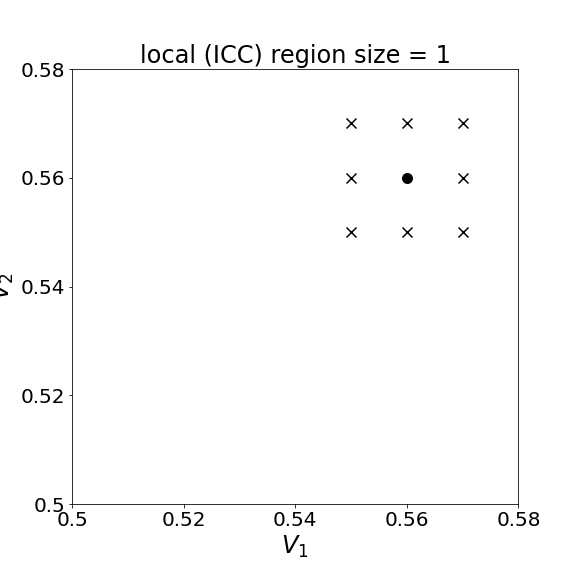
\includegraphics[width=0.3\textwidth]{images/local_size_1.png}
%     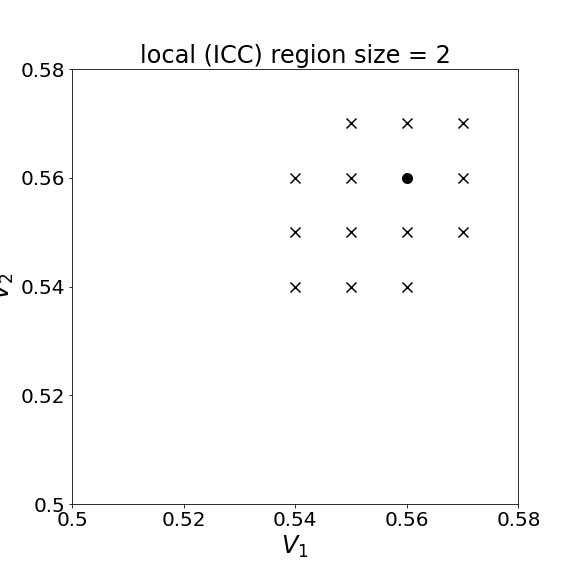
\includegraphics[width=0.3\textwidth]{images/local_size_2.png}
%     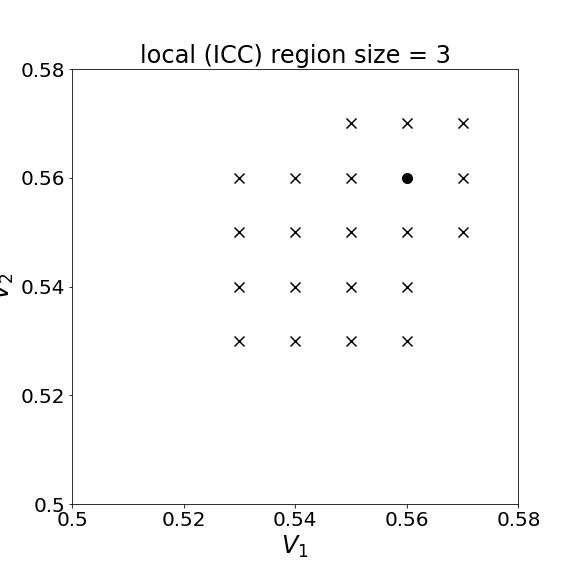
\includegraphics[width=0.3\textwidth]{images/local_size_3.png}
%     \end{center}
    
%     \vspace{1mm}
%     \raggedright{\small {\sc Figure \refstepcounter{fig}\thefig\label{fig:sim1}:} We iteratively grow the local region of the discretized type space checked for downwards-sloping constraint violations. Notice that immediately adjacent (ICC) constraints are always checked ($\times$) when the local region increases in size around a point ($\bullet$).}
% \end{figure}


% Belloni et al. \autocite*{belloni2010multidimensional} use a plane-putting algorithm which works with a randomly chosen subset of incentive-compatibility (ICC) and Border (B) constraints at each iteration. They provide an efficient reduction in the growth in $T$ of the Border constraints (B) from $O(2^{T^J})$ to $O(T^J \log(T^J))$ \autocite[Lemma 10]{belloni2010multidimensional}. We adopt their solution to checking (B) constraints; however, our approach to checking (ICC) constraints involves iteratively growing the `local' region of the type space around each point $v$ in the discretized set of types $V_T$. We do two things. First, all the immediately adjacent points in the discretized type space are always checked for incentive compatibility. Secondly, downwards-sloping points in the discretized type space are also checked. Furthermore, the downwards-sloping region of the type space grows until all (ICC) constraints are ultimately satisfied. This procedure is illustrated visually in Figure \ref{fig:sim1}. Thus, for a fixed-size local region around each point in the discretized type space, we first satisfy \textit{local} (ICC) and (B) constraints as in the iterative plane-cutting algorithm of \autocite{belloni2010multidimensional}. Then we run the separation oracle with \textit{all} (ICC) and (B) constraints. We then restart the solver with any previously violated constraints, this time increasing the size of the local region around each point in the discretized type space. This procedure iterates until no constraints are violated. This modified version of \autocite{belloni2010multidimensional}'s algorithm is described in Algorithm \ref{alg:1}.

% \begin{figure}
%   \centering
%   \begin{minipage}{.7\linewidth}
%     \begin{algorithm}[H]
%     \caption{Iterative plane-cutting algorithm with local and downwards-sloping (ICC) constraints}\label{alg:1}
%     \SetAlgoLined
%     % \KwData{$x=1$}
%     % \KwResult{$y = x^n$}
%     % $\text{local_size} = 1$\;
%     $L = 1, S = \emptyset, A = \emptyset, \overline{OPT} = \infty$\;
%     \texttt{violated\_any\_icc} $\gets $ TRUE\; 
%     \While{\texttt{violated\_any\_icc}}{
%         \texttt{violated\_local\_icc} $\gets$ TRUE\; 
%         \While{\texttt{violated\_local\_icc}}{
%           $k = 1, A^k = A, S^k = S$\;
%           Solve the linear program associated with $S^k$. Let $OPT^k$ denote the optimal value.\;
%           Solve the separation oracle using only local (ICC) constraints in region $L$. Let $A^k$ denote all violated local (ICC) and (B) constraints.\;
%           \If{$A^k = \emptyset$}{
%             \texttt{violated\_local\_icc} $\gets$ FALSE\;
%             Break\;
%           }
%           Select a subset $I^k \subset S^k$ of inactive (ICC) and (B) constraints\;
%           \eIf{$OPT^k < \overline{OPT}$}{
%             $S^{k+1} \gets (S^k \setminus I^k) \cup A^k \cup A$\;
%             $\overline{OPT} \gets OPT^k$\;
%           }{
%             $S^{k+1} \gets S^k \cup A^k \cup A$\;
%           }
%           $k \gets k+1$\;
%         }
%         Solve the separation oracle using all (ICC) constraints. Let $A^*$ denote all violated (ICC) constraints.\;
%         \If{$A^* = \emptyset$}{
%             \texttt{violated\_any\_icc} $\gets$ FALSE\;
%             Break\;
%         }
%         $A \gets A \cup A^*$\;
%         $S \gets S^k$\;
%         $L \gets L + 1$\;
%     }
%     \end{algorithm}
%   \end{minipage}
% \end{figure}

% Our algorithm\footnote{For more details see: \url{https://github.com/jmemich/optimal-auction-multidim}} is written in Python 3.10 and uses Google's open source linear programming solver `GLOP' available in their \texttt{or-tools} package \autocite{ortools}.



\chapter{Reflexive Measurement}\label{ch_reflexivity}

\section{Introduction}

Observer effects in the social sciences go by many names. It is not uncommon to speak of the `Hawthorne effect' \autocite{landsberger1958} or an `experimenter effect' \autocite{rosenthal1966} when the scientist or their science has a causal effect on its target of study. The idea that a measurement can causally affect the phenomenon it investigates is so widespread it is even enshrined in the common adage known as `Goodhart's Law'\footnote{`When a measure becomes a target, it ceases to be a good measure' \autocite{goodhart1984}.}. Observer-type effects turn out to be ubiquitous across the social sciences, recognized and explored by economists and psychologists alike \autocite{friedman1953,gergen1973}. Yet unified philosophical accounts of these diverse effects are rare despite their similar structure and widespread occurrence. For all that social scientists have labored long and hard to mitigate these problems in the course of their research, philosophers of science have neglected to put observer effects into broader philosophical perspective in a manner that can aid the practice of science. 

In philosophy of science, the related idea of a `self-fulfilling prophecy' is an ancient one, going back as far as the story of Oedipus, a mythical ancient Greek king whose best efforts to thwart an oracle's prophecy led to its tragic fulfillment. In its more modern guise philosophers of science have called the idea \textit{reflexive prediction} and its counterpart notion in the social sciences is commonly traced back to sociologist Robert K. Merton's \autocite*{merton1948} discussion of ``self-fulfilling science''. Like observer effects, this concept also captures the idea of the causal impact of science on what it studies. A canonical example of this phenomenon is a bank run: announcing an impending bank run may subsequently incite one. Contemporary philosophers of science have stressed the challenge reflexive prediction poses for theory development and testing in the social sciences (see \cite{kopec2011, lowe2018}). Despite a number of highly distinguished accounts of the idea of reflexive prediction over the past century, the animating idea of the causal effect of science on what it studies and the challenge that it poses is rarely married to a discussion of measurement.

This essay offers a novel account of the concept of \textit{reflexive measurement}. This account captures the salient features of diverse observer-type effects and recovers the intuition that a measurement is reflexive when agents are aware they are subjected to it. This is similar to the well-known idea of `measurement as intervention' in the philosophy of economics (e.g., \cite{morgan2001}). However, unlike existing versions of this account of measurement, a sensitivity to the different ways measurements causally affect their target of study necessitates revising the naive version of the measurement-as-intervention story. Measurements can sometimes fundamentally alter the phenomenon they investigate and other times only affect the data collected, leaving the underlying phenomenon unchanged. For example, in the context of survey research, it is common for respondents to lie about their preferences and opinions but the survey---the measurement instrument---does not causally affect the underlying phenomenon. This appreciation for the different ways measurements can causally affect the phenomenon they investigate sheds light on the deficiencies of the commonly used framework of de-biasing systematic measurement error for addressing the more fundamental problem of reflexive measurement.

% \footnote{Note, the concepts of \textit{performativity} and \textit{reactivity} are very similar and specific differences are discussed where appropriate. Since the point of departure for this work on measurement is the philosophical concept of reflexive prediction this account draws most heavily on those sources. A full discussion of the differences between these related concepts is beyond the scope of this paper.}

Behind the account of reflexive measurement presented here is a reconceptualization of reflexivity in science writ large. Existing philosophical accounts of reflexive prediction would be of considerable help in better understanding the causal effects of measurements on their targets of study were it not for the fact that these insights are specifically tied to an understanding of prediction and rarely given in any form of generality. Thus, it is necessary to step back from specific scientific practices (e.g., prediction, measurement, theorizing) and ascertain how science---broadly understood as a sociological phenomenon---interacts with what it studies. A clear pattern then emerges. The causal effects of science occur only when agents are aware of the science that investigates their behavior. This, in a nutshell, is reflexivity.

% The engagement with scientific literature beyond the traditional domains of economics and sociology paves the way for a potential solution to the problem of lying, misreporting, and withholding data---a common form of reflexive measurement across scientific domains. Drawing on insights from the mathematical and experimental psychologists \autocite{luce95,gergen1973}, designing a measurement to ensure truth-telling is beneficial for those studied yields measurements that are more reliable evidence for the underlying phenomenon. In some sense, in the face of reflexivity, measurements need to be made incentive-compatible or, as I refer to it below, measurements need to be \textit{reflexively optimal}. This idea also complements recent developments in theoretical computer science in the field of incentive-compatible learning and performative prediction \autocite{hardt2016,perdomo2020,cai2015}. The result of this engagement with psychology and computer science is that existing mathematical approaches to dealing with measurement are found to be inadequate. The commonly used framework of de-biasing systematic measurement error can be shown to be insufficient for addressing the more fundamental problem of reflexive measurement.

The essay is structured as follows. In section \ref{sec_lit}, I review the major conceptual innovations on the topic of reflexive prediction by philosophers of science over the past century. Additionally, this review is supplemented by considerations of observer effects by experimental psychologists which are particularly germane to the topic of reflexive measurement. Section \ref{sec_character} collects these accounts and provides a general characterization of reflexivity in science. The central insight of this section is that agents' awareness of their position in a scientific study is the key causal pathway for reflexive effects. With a more general account of reflexivity in hand, the topic of measurement is then explored in section \ref{sec_measurement}. Reflexive measurement is best captured by the measurement-as-intervention view, however, the naive understanding of this position requires modification in light of the distinction between data and phenomena. Section \ref{sec_conc} concludes and offers directions for future work.

\section{Literature Review}\label{sec_lit}

% \footnote{Since \autocite{mackinnon2006} primarily addresses the developments of reflexivity in economics and sociology it suffers from a lack of consideration of reflexivity concerns in empirical psychology, which I explicitly address below. Additionally, the related issue of performativity in computer science is missing from this account.}

The idea that science causally affects its target of investigation has been long discussed in both science and philosophy. In philosophy of science alone, it is known as `reflexivity', `performativity', and sometimes `reactivity'. However, this notion is mostly commonly discussed in the context of scientific theories and predictions. In this section, I provide a stylized overview of the conceptual development of this idea over the past century in order to subsequently develop an account of how measurements can casually affect what they measure. I draw from the well-developed concept of \textit{reflexive prediction} in philosophy of science and supplement this understanding with developments in contemporary science which explicitly concern tackling the problem of the causal effect of science on what it studies. For a more even treatment of the development of reflexivity, albeit with less focus on psychology and contemporary economics, see the historical overview of \autocite{mackinnon2006}.  

Mid-twentieth century philosophical accounts of reflexivity following the sociologist Robert K. Merton's \autocite*{merton1948} seminal account of `self-fulfilling science' are isolated. Karl Popper \autocite*{popper1953} briefly discussed a general formulation of the idea in the context of historicism in philosophy of social science and Ernest Nagel \autocite*{nagel1961} also noted the challenge this posed for theory construction in the social sciences. Subsequent accounts in the 1960s and 1970s focused more narrowly on the causal role predictions in the social sciences have on shaping their own truth-conditions (e.g., \cite{buck1963, romanos1973}). These accounts focus heavily on the formulation and dissemination style (\textit{FD-style}) of the prediction: whether the prediction was published in a newspaper or discussed on cable news, whether the prediction was public or private, etc. To different but ultimately similar degrees, these authors acknowledge that a single prediction will not, by itself, have a reflexive effect independent of how it comes to be known by those it makes predictions about. 

% \footnote{Kopec distinguishes between strong and weak predictions, where `strong' reflexive predictions are predictions that ``switch the truth-value of the prediction'' and `weak' reflexive predictions merely ``change the probability of the predicted event'' \autocite[p1252-3]{kopec2011}. Since the strong reflexive predictions are a subset of weak reflexive predictions, and the latter offers a substantive conceptual innovation over previous accounts, I consider only the latter here.}

These accounts from the 1960s and 1970s understood predictions in science as having a definite true/false truth value. A significant recent contribution by Kopec \autocite*{kopec2011} challenged this view, articulating a conception of probabilistic reflexive predictions. Here, a prediction is reflexive if it changes the probability of the event it predicts. The common use of applied statistics in developing predictions in the social sciences is better accommodated by this account. For example, social scientists have investigated whether public opinion polls indicating a favorite candidate in an upcoming election can increase that candidate's probability of winning \autocite{rothschild2014} and also whether the effects of election forecasts may depress voter turnout \autocite{westwood2020}. A narrow focus on the ultimate truth condition of the prediction misses the ways in which a prediction can nonetheless change individual behavior while leaving the result aggregate phenomena unchanged. Thus, even if a number of voters vote differently in light of public predictions, the result of an election may nonetheless remain unchanged.

A further criticism of existing philosophical work on reflexive prediction is that it fails to account of the idea that certain predictions may be more or less reflexive \autocite{lowe2018,cejka2022}. The ``Mertonian-derived, truth-centric notion of reflexive prediction'' \autocite[p10]{lowe2018} fails to capture the idea that, in some cases, the effect of a reflexive prediction on (even the probability of) an event is ``marginal at best'' \autocite[p8]{lowe2018}. If an impending bank run is announced on the front page of the newspaper of record it has a vastly different effect than on the front page of a local student newspaper. The shift in focus to degrees of reflexivity represents a welcome change in our philosophical understanding of the many ways scientific predictions can interact with the social world. 

Scientists have also developed their own accounts of reflexivity which are notably different from the philosophical views considered above. Contemporary work by economists on reflexivity has ``situate[d] the concept in recent thinking on complex adaptive systems'' \autocite[p331]{beinhocker2013}. This turn towards characterizing reflexivity in terms of systems-type thinking is associated with financier and investor George Soros, who has claimed that understanding the concept of reflexivity has enabled him to profit from his investments in financial markets (see, for example, \cite{soros2013}). On this account, reflexivity is a property of systems. The systems-account emphasizes the interactions between agents and their environment, as well as explicitly conceptualizing agents' goals and cognitive abilities. An upshot of this account is that it arranges different systems along a `spectrum of complexity' \autocite[p337]{beinhocker2013} and enables the comparison of physical, human, and artificial systems in terms of reflexivity and complexity---an unusual feature of accounts of reflexivity.

% \footnote{Experimenter effects also include the presence of implicit cues which can unconsciously influence study participants' behavior. I discuss this subtlety in more detail in Section \ref{sec_measurement}.}

Despite the common focus on reflexivity in economics by philosophers of science issues of reflexivity are found across many other sciences. It is helpful to also draw from the discipline of experimental psychology that has confronted reflexivity as a practical challenge. In doing so it becomes possible to develop a clearer overall picture of the causal effect of science on what it investigates. Phenomena like the `experimenter effect' \autocite{rosenthal1966} and `demand characteristics' \autocite{orne1962} have been well-known for decades and demonstrate the problems that come with either revealing information (e.g., a theoretical premise or expected result) to study participants during the course of research or participants `guessing' the aims and objectives of the study and then adjusting their behavior accordingly. The implications of these findings constitute ``a fundamental difference'' \autocite[p313]{gergen1973} between natural and social science.

Writing about the dangers of theories of psychology that are falsifiable ``at will'' by knowing study participants, mathematical psychologist R. Duncan Luce proposed the `non-oxymoron criterion' \autocite[p3]{luce95} for theory-testing: scientists should be confident that their experimental design allows the theory to be tested despite the subject's knowledge of the theory. In other words, psychological hypotheses should not be able to be confirmed (disconfirmed) by the study participant at will. Psychologists have differed in their recommendations for how to avoid this. On the one hand, considering only ``naive subjects'' ensures that study participants are uninformed and therefore theories can be tested in ``an uncontaminated way'' \autocite[p313]{gergen1973}. On the other hand, we can directly address the self-interest of the subjects such that it ``behooves the subjects to reveal their true preferences'' \autocite[p9]{luce95}. These views complement existing philosophical accounts by highlighting characteristics of study participants (e.g. how informed they are, their goals and desires) which contribute to the reflexivity of science.

% I will return to Luce's comments about study participants ``reveal[ing] their true preferences'' in more detail below. It is worth noting, however, that recent developments in theoretical computer science specifically address reflexivity concerns at the intersection of measurement and prediction by explicitly modeling self-interest when designing algorithms that learn from data. This literature on \textit{incentive-compatible learning}\footnote{This is also sometimes called \textit{strategic classification} \autocite{hardt2016} or \textit{incentive compatible estimation} \autocite{cai2015} or \textit{performative prediction} \autocite{perdomo2020}.} concerns eliciting accurate data when the source of the data has knowledge of the structure of the algorithm and its subsequent use. Examples of this kind of work include eliciting truthful information when people can strategically withhold data \autocite{krishnaswamy2021} and obtaining high-quality data when data collection is costly \autocite{cai2015}. I will cover in more detail the simpler case of \autocite{caragiannis2016}, who consider the classic problem of estimating the population mean of an unknown single-dimensional distribution where samples are supplied by strategic agents who wish to pull the estimate as close as possible to their own value. The approach of this line of work addresses reflexivity directly and attempts to mitigate its effects by explicitly modeling self-interest such it is beneficial to those studied to reveal their true preferences.

% \footnote{In the discipline of computer science reflexivity is commonly studied under the name of \textit{strategic classification} \autocite{hardt2016} or \textit{incentive compatible estimation} \autocite{cai2015} or \textit{performative prediction} \autocite{perdomo2020}.}

In conclusion, it is important to bear in mind that in addition to philosophy of science and economics, disciplines as diverse as psychology \autocite{luce95}, political science \autocite{rothschild2014,westwood2020}, complex systems \autocite{beinhocker2013}, and even theoretical computer science \autocite{hardt2016,perdomo2020} have all grappled with the issue that science causally effects its target of investigation in different forms. As I will detail below, observer effects are ubiquitous across scientific domains and only a broader understanding of these effects can do justice to the complexity of reflexivity in science. This literature review aims to surface some of the common concerns across these disciplines alongside the development of reflexivity as a key idea in contemporary philosophy of science. The next section will tie together these concerns into a general characterization of the concept of reflexivity.








\section{Characterizing Reflexivity}\label{sec_character}

Since almost all explicit definitions of reflexivity are inextricably tied to prediction in this section I propose a characterization of reflexivity which applies to all scientific practices. As such, it will necessarily be broader in scope and include more of scientific practice than is common on other accounts. The proposed account is closer in spirit to earlier attempts to understand reflexivity which attempted to grapple with the ``complicated interaction between observer and observed'' \autocite[p14]{popper1953} at a high level of generality. Drawing from the approach of Grunberg \autocite*{grunberg1986}, the account proposed here sheds light on the causal pathway by which reflexive effects manifest themselves. This serves to fix ideas for the discussion of measurement in subsequent sections. Additionally, this account extends to non-social scientific domains; a feature of reflexivity that has been widely under-appreciated by those who insist the concept uniquely applies to the study of humans and human behavior.

The motivating question for this more general account is: which scientific practices might be reflexive? All conceptions of reflexivity considered in the preceding section implicitly rely on a view of science that encompasses the social interaction between `observer and observed' \autocite{popper1953} or `scientist and study participant'\autocite{gergen1973, luce95}. A broad view requires us to consider science as a sociological phenomenon and allow our characterization of reflexivity to include facts concerning how the science in question interacts with its target of study. Who the scientist is or what institution they work at can have an outsized impact on the results of a scientific study. This is, effectively, a more general formulation of the `formulation/dissemination-style' (\textit{FD-style}) of reflexive predictions \autocite{romanos1973} which naturally extends to other scientific practices like measurement.

However, adopting broader sociological considerations is no small requirement. This means that irrespective of whether a specific scientific practice is known, the mere knowledge of the institution that carries it out can be sufficient to elicit a reflexive effect\footnote{There are even collateral effects from neighboring institutions or scientific practices. These are explored in the case of measurement in example \ref{ex_census}.}. Consider that when Google dropped its ``don't be evil'' motto \autocite{basu2015} users may have felt the need to change their behavior when interacting with Google's products. Even without knowing the specific scientific practices Google was carrying out to investigate their users' behaviors, this might---in the broad sense of being a social interaction between observer and observed---constitute an instance of reflexivity for Google's study of its own users.

This further entails that the private/public distinction that animates so much of the reflexive prediction literature is no longer helpful (e.g., \cite{buck1963,romanos1973,grunberg1986}). To see this consider the following example (adapted from \cite{grunberg1986}):

\begin{example}[Sumerian Economic Forecasts]
The current Chairman of US Federal Reserve Jerome Powell delivers the Federal Reserve's annual economic forecasts on national television in ancient Sumerian with a presentation in cuneiform characters.
\end{example}

\noindent Since, effectively, no one understands ancient Sumerian the forecast would be considered private. Setting aside the issue of market overreactions (e.g., \cite{debondt1985}), this would be an unprecedented action for a Chairman of the US Federal Reserve and may undermine investors' faith in the competence of major US financial institutions. This should constitute an instance of reflexivity in the same way that Google changing its motto should: the broader sociological context of a scientific practice can have enormous causal impacts on what it investigates.

The causal effect that science has on its target of study is clearly at the heart of all conceptions of reflexivity. On an overly simplistic view, reflexivity can even be understood as: the explicans causally affects the explicandum. Some kind of causal effect is clearly a necessary condition for the occurrence of reflexivity---on this, all philosophical accounts agree. But accounts of reflexivity differ in how they approach this. On one view, reflexivity is understood as a causal effect with a counterfactual component \autocite{romanos1973,buck1963}. Another view emphasizes the causal effect of reflexivity as a stochastic phenomenon. A reflexive prediction, for example, changes the probability of an event occurring \autocite{kopec2011} and can even be ascertained by a test of statistical significance \autocite{cejka2022}. A different kind of account gives definitions of reflexivity which omit causal language altogether in favor of clearly specifying the pathways along which the causal effects of reflexive science play out. Thus, for example, a reflexive prediction is ``an utterance... made public in a language in terms that can be understood by the agents to whose behavior it refers and who therefore can by their actions either falsify or fulfill it'' \autocite[p476]{grunberg1986}\footnote{Alternatively, ``in order to be reflexive it is sufficient for a public prediction to be partially believed'' \autocite[p484]{grunberg1986}.}. A distinct advantage of this final approach is that it subsumes the causal effects of science on what it studies by specifying the mechanism by which agents might come to frustrate or fulfill a scientific prediction.

Before offering my own version of this type of account of reflexivity, it is important to be clear about the nature of ``agents'' that constitute part of the phenomenon investigated by scientists. In my view, the systems account of reflexivity (e.g., \cite{beinhocker2013,soros2013}) correctly captures the important features of agency, including agents' goals, cognitive capacities, and actions within the scope of a definition of reflexive system\footnote{However, I do not believe the most promising path towards characterizing reflexivity is to ``situate the concept in recent thinking on complex adaptive systems'' \autocite[p331]{beinhocker2013}. Although there are undoubtedly good reasons to think about reflexivity in this manner for large-scale, complex phenomena like financial markets, the `systems' approach is ill-suited to capture small-scale scientific investigations like laboratory studies \autocite{luce95} and individual medical diagnoses \autocite{hacking1995}. Especially since some systems accounts of reflexivity (e.g., \cite[p332]{beinhocker2013}) require that all reflexive systems be complex systems.}. It is important to consider why this is particularly helpful. Firstly, note that reflexivity may characterize sciences that investigate collections of humans: organizations, governments, firms, etc., which act with a singular purpose. These can be modeled as agents. Secondly, it would be philosophically underwhelming to propose an account of reflexivity which rules out interesting cases like missiles \autocite{grunbaum1963} or thermostats \autocite{beinhocker2013} simply because the only agents to which the concept of reflexivity applies are human beings. It is desirable to simultaneously capture the intuition that there is something particularly philosophically interesting about the problems faced by social science but also that we should be open to discovering these problems in other scientific domains. Although there will certainly be disagreement over what constitutes agency, this ambiguity is a deliberate feature of the account presented here.

The account of reflexivity proposed here requires that the causal effect of observation or measurement or prediction---any form of scientific practice---on the target of inquiry be mediated through the awareness of the agents that constitute part of the phenomenon under investigation. Here, I am trying to generalize to all scientific practices the idea that the mechanism for a prediction to be reflexive is for it to be ``partially believed'' \autocite[above]{grunberg1986}. It is meaningless to speak of ``belief'' in the context of measurement. Some minimal degree of awareness of being observed is the relevant necessary condition for reflexivity. This requirement widens the scope of what is to be considered reflexive, as did the move to include the broad sociological context of scientific practice beyond, for example, individual public predictions. What ultimately matters for reflexivity is not how a given prediction, theory, or measurement was published or disseminated (i.e., its \textit{FD-style}) but instead that the agents came to learn it. 

The implications of this novel understanding can be fully seen in the following example.

\begin{example}[Stoplight Example]
A researcher aims to measure traffic patterns at an intersection. They stand on the side of the road noting the presence and absence of cars waiting at a stoplight. Inadvertently, however, they keep stepping on the cable that powers the stoplight, affecting the frequency with which the stoplight changes color.
\end{example}

\noindent In this example, although the scientist causally intervenes in the target system they are seeking to study, the effect of this causal intervention is not a function of the agents' awareness of the science or scientist that studies their behavior. Thus, if the drivers of the cars (i.e., the agents) are unaware of the science that investigates their behavior, then the scientific study is not reflexive. This extends to the institution that the scientist is working for: if the agents are unaware not only of the scientist at the stoplight but of the broader sociological context in which they conduct their science, only then is science truly non-reflexive. As noted above, large corporations like Google and intelligence agencies like the CIA, which are often jokingly considered omniscient, will elicit reflexive effects even if the specific scientific investigations they carry out are unknown to those they study.

It is tempting to argue that awareness is also sufficient for reflexivity, however, I believe this kind of precise definition leads to the consideration of unhelpful counterexamples.

\begin{example}[Alien Social Science]\label{ex_aliens}
Assume only one species of aliens exists and consider that their alien social science which investigates human behavior on earth is entirely undetectable by us (i.e., has no causal impact we can discern). Despite this, some members of the public believe that aliens are real. Perhaps they have they have filled their imaginations with stories of Area 51 or watched too many \textit{X-Files} episodes. Thus, they adapt and change their behavior in ways they think might frustrate alien social science.
\end{example}

\noindent Since the account here argues in favor of considering collateral effects of institutions on earth (e.g., the FBI, Hollywood, etc.) a key part of reflexivity, then the alien social science is reflexive despite the lack of \textit{any} causal effect on the phenomena it investigates.

This surprising conclusion is a feature of the inclusion of collateral reflexive effects (from, say, neighboring scientific institutions with bad reputations as covered in example \ref{ex_census} below) in the proposed characterization of reflexivity. When coupled with awareness as the appropriate causal pathway for mediating reflexivity renders the range of cases to which the designation of reflexivity applies very broad. This is partly by design: the goal of this account is to extend existing ideas and intuitions about reflexivity to (potentially) cover all scientific practices. Even Ian Hacking's \autocite*{hacking1995} seminal account of the causal effects of scientific theories themselves cannot be included in a discussion of reflexive predictions without significantly changing the scope of the argument (and all the relevant definitions of reflexive prediction). Treating awareness as a sufficient condition for reflexive entails that a science can be reflexive without causally affecting its target of study, a conclusion completely at odds with the animating idea of the characterization given here.

The characterization of reflexivity proposed here entails that almost all social scientific practice is reflexive. This feature of my characterization of reflexivity might strike the reader as unwelcome. Yet narrowly defining reflexivity in terms of ``causal factors'' \autocite{romanos1973,buck1963} or ``changes in probability'' \autocite{kopec2011} to pick out particular instances of reflexivity lands philosophers of science in the awkward position of assuming the role of scientists: determining what is and isn't reflexive in virtue of measurable effects. Moreover, recent developments in how to think about reflexivity emphasizing that reflexivity is a matter of degree \autocite{lowe2018} lend support to the idea that even minimal reflexive effects are still worthy of inclusion in the definition of reflexivity.

Ultimately, if reflexivity is defined by its effects it lands us with an arbitrary delineation of the term. Consider that a definition using the language of ``causal factors'' and ``changes in probability'' entails that the same prediction uttered in two almost identical circumstances might nonetheless result in one being reflexive while the other is not. These differing circumstances could be different days of the week, neighboring geographic regions, or even just differ in as much as a single study participant. Even more problematic is the fact that the absence of a discernible reflexive effect does not indicate the absence of reflexivity. A public prediction might result in exactly the same pattern of behavior (or probability of its occurrence) but the motivations for carrying out the behavior may have completely changed as a result of the prediction. A focus on the causal pathway by which reflexivity manifests allows philosophers of science to sidestep issues with ascertaining whether there is an appropriately reflexive causal effect for a given scientific practice. 

Thankfully, social scientists are increasingly aware of the reflexive effects of their science. Contrary to earlier philosophical accounts of reflexivity which could only find a ``a great deal of anecdotal evidence'' \autocite[p487]{grunberg1986} for the existence of reflexive predictions, a serious effort has been made to investigate the effects of public predictions in areas like election forecasting. Well-known election forecasts in the United States like Nate Silver's 538 website\footnote{\url{https://fivethirtyeight.com}} which get national press coverage are now being investigated for their effects in depressing voter turnout \autocite{westwood2020}. Additionally, opinion polls indicating a favorite candidate in an upcoming election can increase the probability of that candidate winning \autocite{rothschild2014}. The advantage of taking seriously the recommendation to treat reflexive effects as varying by degree \autocite{lowe2018} is that it leaves open the possibility of acknowledging that almost all social science is reflexive, though much of it might have barely any effect at all. Philosophers can offer a clear account of reflexivity and let scientists determine where it is appropriate to worry about it.

In summary: I provided a sociological picture of scientific practice, whereby a reflexive scientific practice can causally affect its target of inquiry when the cause is mediated through the agents' awareness. Although this condition is necessary for reflexivity, and, indeed, it is often sufficient, a definition should be avoided: it adds little to our scientific and philosophical understanding of a wide-ranging, complex phenomenon and only serves to distract us with far-fetched counterexamples. Furthermore, it is important not to define reflexivity by its effects. Today's election forecasts are reflexive, as are tomorrow's---irrespective of whether one elicits a causal effect and the other does not. What matters is whether the agents that comprise the phenomenon under investigation are aware of the prediction (and so it goes for measurement, etc.). Philosophers of science should let scientists determine the effects of reflexivity; our role is to clarify the phenomenon of reflexivity as one that does or does not apply to various scientific practices and domains. However, before instantiating this account in the novel context of measurement, it is important to consider the implications of this view for what kinds of science are reflexive.




% \section{Reflexivity \& Social Science}\label{sec_social_science}

% An upshot of the preceding section is that it engenders a reconsideration of the claim that reflexivity is exclusively a property of the social sciences and therefore can be used as a demarcation criterion between scientific domains. It has been commonly asserted by philosophers (e.g., \cite{buck1963,popper1953}) that reflexivity (in some form) ``is a phenomenon proper to the social sciences'' \autocite[p484]{grunberg1986}. Against this position, some have argued that feedback systems like missiles should be considered reflexive \autocite{grunbaum1956,grunbaum1963}. Contemporary research has eschewed debates about demarcation (e.g., \cite{lowe2018,kopec2011,cejka2022}), however, the use of reflexivity as a demarcation criterion between scientific domains remains undisputed. I do not wish to challenge the intuition that the study of living human beings and their behavior presents challenges not found when studying stars or atoms. This intuition strikes me as entirely correct. However, the characterization of the preceding section offers a means of reconciling this intuition with a more nuanced understanding of where reflexivity does and does not apply, ultimately entailing a rejection of it as a phenomenon ``proper'' to the social sciences.

% It is never entirely clarified what is meant by ``social science'' throughout these arguments. Clearly, disciplines like economics, political science, and sociology are all included. On the side of ``natural science'', presumably, we have subjects like physics, chemistry, and biology. Through these (and a few other) examples, this division of scientific domains effectively takes place at the level of academic departments. This is regrettable for two reasons. First, reflexivity does not apply uniformly within even a single social science and, secondly, interdisciplinary subjects like cognitive science are left out entirely.

% Before considering the possibility of reflexive natural science, it is helpful to briefly dwell on the nature of agency alluded to in the preceding section. The picture of agency I'm relying on in my account of reflexivity is drawn from those who approach the study of reflexivity using the framework of complex systems (e.g., \cite{beinhocker2013,soros2013}). These accounts rely on a system-level description of phenomena (like financial markets) which includes agents with goals, available actions, variable cognitive functions, and even ``internal models'' of how their actions yield consequences \autocite[p331]{beinhocker2013}. My account stressed agents' awareness but eschewed the stronger criterion of ``understanding'' is used in some accounts of reflexive prediction (e.g. \cite{grunberg1986}). My aim is to capture the idea of an observer effect in its broadest possible formulation. Reflexivity also requires agents---in some form or other---to be part of the phenomenon under investigation. I think it uncontroversial to say the study of stars and atoms can never be reflexive: these phenomena are simply not agents in any relevant sense of the word. Thus, the proposed account of reflexivity in some sense `lines up' with the intuition that much of the social sciences are reflexive whereas much of the natural sciences are not.

% However, we must not be too quick to jump to conclusions about the natural sciences; without a closer consideration of entities that meet the standards for agency, we should not conclude that natural sciences are entirely non-reflexive. Most notably, I think one scientific domain that most certainly meets the criteria for reflexivity is ecology: in particular the study of primates. Primates are most certainly aware of being observed. There is evidence of observer effects when studying Capuchin monkeys \autocite{metcalfe2022} and there is even evidence it can be mitigated by habituation \autocite{crofoot2010}. The study of primates presents an excellent case for reflexivity: they have different goals, levels of awareness, and cognitive faculties than humans, and thus reflexivity entails entirely different behaviors than, say, humans reacting to election forecasts. Thus, it is possible to see the study of the natural world and the social world along a continuum where it is the differences in the types of agents studied and the causal interactions between scientists and their target of study that make for differences in the reflexivity of science.

% As alluded to above, fields like cognitive science and artificial intelligence might include reflexive scientific practices. Ultimately, the inclusion of fields like these in the category of reflexive sciences hinges on the appropriate definition of agency and awareness. Counterexamples like missiles \autocite{grunbaum1956,grunbaum1963} and thermostats \autocite{beinhocker2013} to definitions of reflexivity which entail that only social scientific domains are reflexive prompt interesting questions about the nature of agency and its relation to awareness of scientific practices. These counterexamples are clear instances of causal feedback loops: they are self-correcting in the sense that once a goal is specified, these systems will take actions to change their environment to satisfy the goal\footnote{Furthermore, these kinds of systems may soon represent some form of scientific practice: the growth of automation in science means that in the not-too-distant future, it is entirely plausible that major policy decisions may be taken autonomously (e.g., \cite{zheng2022})}. Doing justice to all potential counterarguments involves giving a comprehensive account of agency (and also awareness), which is beyond the scope of this paper. However, my goal here is to bring to the reader's attention that the broad formulation of reflexivity in terms of agents' awareness encompasses scientific domains of study beyond the social sciences. 

% The goal of this section was to argue that the traditional conception of reflexivity as only applicable to the social sciences is incorrect and ultimately misguided. If the age-old division between ``social'' and ``natural''  science is based on the reflexivity of one (but not the other) then this understanding of the division reflects anachronistic thinking. Natural scientific domains like ecology are clearly reflexive. Furthermore, as the previous examples of thermostats and missiles show, reflexivity hinges on a definition of agency and what it means for agents to be ``aware'' of scientific practices. Ultimately, the framework developed here to better understand reflexivity allows us to extend considerations of the causal feedback effects of science to entirely new domains and forms of scientific practice.




\section{Reflexive Measurement}\label{sec_measurement}

% \footnote{I make the minimal assumption that measurement requires data collection and focus on this aspect of measurement throughout this section. This aspect of measurement is common to all philosophical accounts of measurement I have been able to find. Additionally, this understanding of measurement remains neutral with respect to questions on operationalism and conventionalism, realism and measurement, model-based accounts of measurement, etc (see \cite{sep-measurement-science} for an extended discussion of philosophical accounts of measurement in science).}

Despite the enormous amounts of ink spilled by scientists lamenting the challenges of collecting accurate data from study participants in laboratories and surveys, this aspect of scientific practice has been mostly overlooked by philosophers of science working on reflexivity. In this section, I instantiate the concept of reflexivity in the context of scientific measurement. Note, however, no new philosophical account of measurement is given in this section. Instead, the discussion of measurement sits closer to how a scientist encounters it. The focus of this section is on data collection since no measurement is possible without it. The heuristics to which scientists avail themselves to understand observer effects are exactly the level at which this account is pitched: it is an attempt to unify these solutions under a single philosophical perspective.

% \footnote{Note, whether or not the following observer-type effects are general and to what extent they replicate is an active area of research in every scientific domain that discovers any hint of these effects. However, consideration of these effects is considered standard practice in `good study design' across scientific fields, so much so that they are commonly found in textbooks across the social sciences (see, for example, \cite{groves2011,stantcheva2022,goodwin2009}).}

It is worth beginning with what is known about observer effects by scientists working across different fields. In its most general formulation across the social sciences, this is known as the `Hawthorne effect' (see \cite{landsberger1958}) or `experimenter effect'\footnote{Though experimenter effects occur when study participants are not explicitly aware of them (e.g., through implicit cues that are registered subconsciously) the focus of this section is the reflexive effects of measurement. As per the characterization in the preceding section, these are only the effects that participants are aware of.} \autocite{rosenthal1966}, where humans react to being observed and change their behavior in light of this observation. This general effect has been given a myriad of more specific formulations in different circumstances. To name a few of the most common found in scientific experiments: `demand characteristics' are a phenomenon where study participants in an experiment act in ways they think the scientist desires \autocite{orne1962}; the `Pygmalion effect' is a psychological phenomenon whereby high expectations lead to improved performance \autocite{rosenthal1968}; the `John Henry effect' concerns the actions that study participants take on learning they are placed in a control group (as opposed to a treatment group) to overcome the disadvantage of being an experimental control \autocite[p399]{dictionary_psych}. Outside of experiments, observer effects are commonly found in applied survey research: `priming' occurs when a survey asks leading questions which can skew survey responses \autocite[\S 6.2]{stantcheva2022}; additionally, `social desirability bias' is the phenomenon of surveys respondent lying or not sharing sensitive opinions  \autocite{krumpal2013}. Even `Goodhart's Law' has its origins in the challenges faced by economists measuring economic indicators to set monetary policy \autocite{goodhart1984}.

These disparate concerns all have the same root: the causal effects of scientists and their science on the target of study. Crucially, the kind of effects cataloged above are all mediated through the awareness of the agents studied. Study participants in laboratory experiments and respondents taking surveys are all fully aware of their role in scientific studies. Indeed, this is required for ethics approval. Thus, reflexive measurement can best be understood as the idea of `measurement as intervention', which has long been known in philosophy of economics. Writing about the role of measurement instruments in economics, Mary Morgan shrewdly writes:
\begin{quote}     
    ``The ways in which the economic body is investigated and data are collected, categorized, analyzed, reduced, and reassembled amount to a set of experimental interventions---not in the economic process itself, but rather in the information collected from that process.`` \autocite[p237]{morgan2001}
\end{quote}
\noindent However, Morgan contends that the interventions do not causally affect the ``economic process itself'' and instead affect the ``information collected from that process''. In the context of much of contemporary economics, this seems apt, however, more broadly this account fails in other settings\footnote{See Example \ref{ex_spe}. I explore this in more detail below.}. This insightful intuition about measurement instruments can be better appreciated by further considering the difference between `data` and `phenomena'.

% \footnote{Contemporary philosophical work on reactivity in similar contexts of measurement (e.g., \cite{runhardt2023}) draws on a conception of reactivity developed by \autocite{golembiewski1976} which is an exemplar of this first type of reflexive measurement: a measurement which causally affects the underlying phenomenon.\label{fn_reactivity}}

A helpful philosophical account of the difference between data and phenomenon was developed by Jim Woodward \autocite*{woodward1989}. Phenomena are ``relatively stable and general features of the world which are potential objects of explanation and prediction by general theory'', whereas data ``by contrast, play the role of evidence for claims about phenomena'' \autocite[p393-4]{woodward1989}. What matters in any scientific description or analysis of a phenomenon is that ``the data should be \textit{reliable evidence} for the phenomena in question'' \autocite[p398, emphasis original]{woodward1989}. Furthermore,
\begin{quote}
  ``Scientific investigation is typically carried on in a noisy environment; an environment in which the data we confront reflect the operation of many different causal factors, a number of which are due to the local, idiosyncratic features of the instruments we employ (including our senses) or the particular background situation in which we find ourselves.'' \autocite[p398]{woodward1989}
\end{quote}
\noindent In the context of the account of reflexive measurement introduced above (i.e., `measurement as intervention'), data reflect the operation of measurement instruments and the broader sociological context in which scientists administer their measurement. Crucially, however, the causal effect of the measurement on what is being measured might affect the underlying phenomena itself and/or the data collected about it. To see this more clearly, I now consider two concrete examples.

To make vivid how an act of measurement may cause the phenomena under investigation to change, consider the following well-known experiment by psychologist Philip Zimbardo:

\begin{example}[Stanford Prison Experiment]\label{ex_spe}
In 1971 a psychologist recruited participants for a ``psychological study of prison life'', which was a planned one-to-two week experiment that simulated prison life (see \cite[\S 2]{spe} for details). The goal was to assess the psychological effects of becoming a prisoner or prison guard.
\end{example}

\noindent A full account of the Stanford Prison Experiment can be found in \autocite{zimbardo2008}. It was prematurely ended after only 5 days since ``prisoners were withdrawing and behaving in pathological ways, and... some of the guards were behaving sadistically'' \autocite[\S 8]{spe}. The ethics of this kind of experiment have been questioned: participants who simulated prisoners were deliberately made to feel humiliated \autocite[\S 3]{spe}. Zimbardo's method of investigating the effects of simulated prisoner-guard has also been criticized as poor scientific practice \autocite{letexier2019}. Ultimately, it is abundantly clear that if the effects of the experiments are so pronounced as to induce a study participant to ``[break] down and began to cry hysterically'' \autocite[\S 8]{spe} then the measurement is reflexive in the sense of causally affecting the underlying phenomenon.

In contrast, a reflexive measurement can causally affect the data collected by a scientist without altering the underlying phenomenon under investigation. This is common in almost all forms of survey research where participants have the opportunity to lie or misrepresent their opinions. Here, a sensitive issue like the approval of a controversial political figure may be unaffected by a reflexive measurement but the data collected may be influenced by the study participants' reluctance to truthfully report their views. I believe this is the most promising way to realize Mary Morgan's insight that measurements of the economy are interventions ``in the information collected from that process''. 

The next example provides a concrete case where the social context of the scientific practice can create exactly this kind of effect.

\begin{example}[2020 US Census]\label{ex_census}
    In the run-up to the 2020 US Census, then-President of the United States Donald Trump made repeated remarks about the possibility of adding a citizenship question to the census (see \cite{blake2022}). Subsequently, the Hispanic response rate was more than three times lower on the 2020 census than on the 2010 census\footnote{See Appendix 1 for calculation of this figure.}.
\end{example}

% \footnote{\color{red}TODO ``The general tendency in “do not know” responses increased proportionally to the sensitivity of the issue.'' \autocite{dadabaev2007}.}

\noindent This example highlights an important and often overlooked facet of scientific practice: \textit{who} the scientist is or \textit{what} institution they represent can have direct consequences on their ability to investigate phenomena in the face of reflexivity. Here, explicit condemnation of undocumented immigrants by former president Donald Trump likely had a causal role in more than tripling the number of those of Hispanic origin in the US who didn't complete the 2020 census compared to 2010. The underlying phenomena of interest investigated by the census (e.g., respondent's age, gender, income, etc.) don't change but the data collected are influenced by a powerful leader with the ability to use census data to create policies that leave undocumented immigrants worse off by deporting them.

% The sociological picture of science presented in the previous section which focuses on scientific practice is central to the view of reflexive measurement proposed here. Institutions, people, expectations, etc all matter in changing the calculus of costs and benefits that study participants carry out when providing data. Though measurements can alter an underlying phenomenon (as in the Stanford Prison Experiment example above) this is often considered poor research design and scientists typically seek to eliminate these effects insofar as they are able to. Mitigating reflexive measurement effects on the data is a more difficult proposition that requires reasoning about agents' goals and cognitive abilities. Given the challenges associated with overcoming this latter kind of reflexive measurement issue, I now turn to concrete proposals from across scientific domains developed specifically to collect data that are more ``reliable evidence'' for the phenomenon in question.

% \section{A Concrete Proposal}\label{sec_proposal}

% Measurement without care on behalf of scientists to mitigate observer-type effects on data collection---even if the underlying phenomenon is unchanged---will result in data that are not reliable evidence for the phenomenon in question. The resulting inferences and predictions will be artifacts of the measurement rather than accurately represent the phenomenon under investigation. I believe the solution to problems of reflexive measurement lies in developing a scientific understanding of how our measurements affect the incentive structures of the agents we collect data about. The rest of this section collects and synthesizes disparate observations from scientists dealing with observer effects to motivate a concrete approach for modeling the reflexive causal effects of measurement instruments.

We can be clearer about the particular phenomenon of reflexive measurement where a measurement casually affects either the data collected or the underlying phenomenon. The change in the distribution of the sample resulting from a reflexive measurement can be thought of as a kind of \textit{distribution shift}\footnote{This language is commonly used in computer science in the related context of \textit{performative prediction} \autocite{perdomo2020}.}. The distribution shift of the sample represents its departure from the population-level data model. The measurement itself is an intervention that, for example, affects study participants' willingness to lie or conceal information in the face of a prying scientist. Notice this intervention only affects the sample since it is only the sample that is subjected to the measurement. Thus, this kind of reflexive measurement can be thought of as a kind of distribution shift where the sample distribution no longer represents the population distribution. 

By way of contrast to this understanding of reflexive measurement, it is helpful to consider the commonly used approach of `de-biasing' systematic measurement error. The systematic component of measurement error always occurs, with the same value, when the instrument is used in the same way in the same case (see \cite{tal2019}). Thus, for example, we might say the systematic component of measurement error for a poorly worded survey question on political attitudes occurs when the responses are, for example, `X\% more left/right-leaning'.

\begin{example}[De-biasing measurement error]\label{ex_debias}
Consider the case of a survey question asking about presidential approval in the US, which was answered by $N$ respondents. The data $X_1, \dots, X_N$ are assumed to come from a Gaussian distribution with unknown mean $\mu$ and variance $\sigma$. A scientist might then want to learn the value of $\mu$. The statistical error associated with each random variable $X_i$ is decomposed into a random and systematic component:

\begin{equation*}
    \epsilon_i = \epsilon_i^{\text{random}} + \epsilon^{\text{systematic}} =  \mu - X_i
\end{equation*}

\noindent Given further knowledge of the particulars of this domain of social inquiry, the scientist might impose additional assumptions about, for example, the shape of the distribution of the errors, or their covariance structure. These assumptions capture some of the flaws associated with a particular measurement instrument or measurement process. Ultimately, a scientist could make a post hoc correction for measurement error by subtracting off (often called `de-biasing') the systematic component of the error:

\begin{equation*}
    X_i^{\text{new}} = X_i + \epsilon^{\text{systematic}}
\end{equation*}

\noindent Which will provide a more accurate (i.e., less biased) estimate of $\mu$.
\end{example}

This example is paradigmatic of how measurement error is handled in the social sciences. The measurement instrument is biased and assumed to interact with those it's intended to measure in a uniform manner. The post hoc measurement error correction\footnote{Since $\epsilon^{\text{systematic}}$ is unknown a correction is only possible with an estimate of this quantity. Ascertaining whether or not this estimate is unbiased with respect to reflexive measurement effects is non-trivial. For a related discussion of this problem in the context of reflexive prediction see \autocite{cejka2022}.} can be read as, effectively, claiming the underlying data generating process measured by the instrument is actually a Gaussian distribution with mean $\mu - \epsilon^{\text{systematic}}$ and variance $\sigma$ once the causal effect of the instrument on the data generating process is accounted for.

However, this kind of correction presumes the underlying sample distribution remains unchanged in the face of reflexivity except for a difference in means. In many settings, this may be a reasonable and accurate assumption. However, this framework of de-biasing error cannot account for changes in the higher moments (e.g., variance, skew, etc.) of the underlying distribution. Moreover, the type of statistical distribution itself might change, often considerably, as a result of the measurement. In example \ref{ex_census} above, some Hispanic subgroups who felt threatened by the increased condemnation of undocumented immigrants might be entirely missing from the resulting data. The problem of reflexive measurement is a deeper one than the framework of measurement error allows. This understanding of reflexivity and measurement error also applies more generally to de-biasing corrections in reflexive prediction \autocite{cejka2022}. Sometimes these are appropriate responses to the problem of reflexivity in measurement, however, they are not a substitute for a general understanding of the problem of distribution shift induced by a measurement.

\section{Distribution Shift and Mechanism Design}\label{sec_reflex_mechdes}

How best then to correct the sample distribution shift that results from a measurement? I think it is instructive to return to the observation by psychologist R. Duncan Luce who, when he advocated the `non-oxymoron criterion' for theory-testing discussed above, noted that studies should be designed such that it ``behooves the subjects to reveal their true preferences'' \autocite[p9]{luce95}. The account of reflexivity in the previous section focused on the causal pathway of agents' awareness, coupled with their goals, cognitive capabilities, and the actions available to them. Explicit concern with what agents want facilitates the possibility of designing measurements that induce a distribution shift such that accurate data are collected because it is in the study respondent's best interests.

Thus, we can think about whether measurements are, in a loose sense, incentive-compatible\footnote{This has a specific, technical meaning in the context of mechanism design. Here, I use it in the informal sense.}. Incentive-compatible measurements induce minimal distribution shift such that the data collected are reliable evidence for the underlying phenomenon. This idea is related to that of \textit{performative optimality} developed in \autocite{perdomo2020} to capture the distribution shift caused by performative predictions\footnote{Their proposed definition is one of iterative convergence from model retraining \autocite[Definition 2.3]{perdomo2020}. The use of the word `prediction' should not confuse philosophers: the problem they consider is simultaneously a problem of measurement. Data are collected for retraining after each iteration of the model is deployed.}. Two differences being: the account here presupposes neither a model nor some form of model retraining. A single measurement (a survey, a laboratory experiment, etc) should be designed in such a way as to be \textit{reflexively optimal}. It should induce a distribution that is reliable evidence for the phenomenon under investigation (i.e., the sample distribution should be an accurate representation of the population distribution). Thus, it should incentivize truth-telling, discourage withholding relevant information, etc.

Further departing from \autocite{perdomo2020}, it is helpful to consider reflexive optimality an equilibrium notion\footnote{The equilibrium notion of \autocite[p1]{perdomo2020} ``coincide[s] with the stable points of $[\text{model}]$ retraining'' and does not reflect an understanding of why agents act they way they do. In contrast, recent work \autocite{oesterheld23} conceives of a truth-telling equilibrium in a performative prediction game as one induced by the self-interest of the participants. In the author's view, this latter contribution is the more promising approach to tackling the problem of reflexive measurement.} in the game-theoretic sense (e.g. \cite{nash1950}). This is helpful for two reasons. First, it allows scientists to give an explicit model of agents' motivations and reasoning and how they interact with a measurement. As argued above, this is a key facet of understanding how reflexive science causally affects its target of study. Secondly, it facilitates the application of the techniques of mechanism design\footnote{See \autocite{borgers2015} for an introduction to the topic of mechanism design.} to the problem of designing reflexively optimal measurement instruments. This turns out to be closely related to an active area of research in theoretical computer science called incentive-compatible learning. Here, the choice of statistical estimator or algorithm itself can induce people to adapt their behavior. Thus, it is possible to re-frame the choice of estimator or algorithm as one that induces truth-telling on behalf of those data are collected from. To better understand this approach, consider the following example from \autocite{caragiannis2016}:

\begin{example}[Incentive-Compatible Mean Estimation]\label{ic_estimators}
A statistician is trying to estimate the mean preferred temperature of occupants of a building. A sample of occupants are randomly selected and asked their preferred temperature. Consider the following scenarios.

In one case, each person sampled is told that the estimator the statistician will use for their estimate of the population mean is the sample mean. Notice that if you have a preference for, say, warmer temperatures, you are best off lying about your preferred temperature to raise the sample average. This is because more extreme values will raise the sample average.

Suppose the statistician instead uses the sample median as his estimate of the population mean and this is communicated to each person in the sample. Even if you have a preference for much warmer temperatures, you no longer gain by lying since the median is robust to large outlier values (see \cite{caragiannis2016} for extended discussion of this result).
\end{example}

In example \ref{ic_estimators} above, there is an explicit model of the relationship between the statistical estimator and the data collected in terms of benefits to people (i.e., their utility). The choice of statistical estimator (i.e., measurement instrument) is recast as a game theoretic problem whereby the statistician and the people in the sample play a game. The statistician wants to estimate the population mean. People in the sample will report their preferred temperature truthfully if they stand to benefit from it or can't benefit from lying. Thus, the statistician can use the \textit{sample median} to estimate the \textit{population mean} to achieve reflexive optimality. Note that despite the game-theoretic formulation of the problem the goal of statistical inference remains the same.

In this example, the sample distribution changes as a function of the estimator yet the underlying phenomenon of interest (people's preferred temperature) remains unchanged throughout. The measurement instrument (i.e., estimator) is chosen so as to induce a distribution shift which is more reliable evidence for people's preferred temperature. This framework of incentive-compatible estimators and algorithms has been extended to explicitly causal settings \autocite{toulis2015}, forecasting problems \autocite{roughgarden2017}, and even bandit-type exploration algorithms \autocite{mansour2019}. It makes the strong assumption that study participants know the functional form of the estimator and possess an ability to reason about how the actions they can take ultimately affect their welfare. However, it explicitly models the incentive structures faced by agents whose behavior is measured. This captures the key idea of the proposal that opened the section: scientists need to understand how their measurements affect the incentives of agents they collect data about.





\section{Conclusion}\label{sec_conc}

I have argued for a novel conception of reflexivity that puts the sociological practice of science at the center of our understanding of reflexivity. This move facilitates the consideration of the multitude of ways science and scientists causally affect their target of study. Reflexivity concerns a kind of causal effect that science has on its target of study where agents that comprise the phenomenon of interest are aware of the scrutiny they are subjected to. In the case of measurement, we can distinguish this measurement-as-intervention view by virtue of whether the measurement causally affects the underlying phenomenon or the data collected about it. The correct understanding of reflexive measurement is given by the concept of distribution shift, where the sample distribution is no longer an accurate representation of the population model due to the causal effect of the measurement.

A few points are worth emphasizing. Firstly, scientists who warn of the consequences of observer effects or self-fulfilling science often do not narrowly focus on either measurement or prediction but instead explore and investigate cases where they co-occur. In psychology, researchers \autocite{gergen1973,luce95} consider how revealing a theoretical finding during a laboratory experiment can result in the study participants falsifying (or confirming) the experiment at will. In computer science, researchers have considered the effects of predictions on subsequent data collection \autocite{perdomo2020}. The account presented here offers a more general characterization of reflexivity which is more faithful to its varied manifestations. In my view, large swathes of science are entirely reflexive and yet, perhaps surprisingly, reflexive effects are often quite minor. Thankfully, scientists are increasingly aware of this phenomenon and have begun investigating specific occurrences of reflexivity in a far more thorough capacity than philosophers (e.g., \cite{rothschild2014,westwood2020}).

Additionally, an upshot of the characterization given in section \ref{sec_character} is that the terrain of the discussion concerning the presence of reflexivity, reactivity, and performativity in a scientific domain should shift from an antiquated ``social'' versus ``natural'' science framing to one instead marked by a deeper appreciation for the nature of agency. The question `is a science reflexive?' is transformed into `what is the nature of agency?' in virtue of the concern with awareness as the causal pathway along which reflexive effects materialize. Where opinions differ on the nature of agency, so too will they differ on the designations of reflexivity. Counterexamples to purely social scientific definitions of reflexivity like missiles \autocite{grunbaum1956} and thermostats \autocite{beinhocker2013} make this point abundantly clear. In my view, this is a welcome change. It moves from treating an existing academic division of labor as a primordial categorization of scientific practice to one instead informed by careful study of differing targets of inquiry.

Two extensions to the line of research initiated here are clear. Firstly, it is worth noting a significant omission from the present account is that of qualitative social science. Qualitative research techniques across the social sciences have become increasingly sophisticated (see, for example, \cite{king2021}). Further research outlining how the account presented here interacts with scientific practices like structured interviews and ethnographic research would be welcome. Secondly, it is an interesting and challenging proposition to extend the understanding of reflexive measurement as distribution shift to scientific practices like prediction and theory development. As introduced here, the concept is bound up with data collection, and extending the account here for other scientific practices may yield insights that aid scientists in overcoming the reflexive effects of science.

Almost half a century ago, political scientist Christopher Achen lamented the lack of understanding social scientists possess concerning how their measurement instruments investigate the world. He wrote:

\begin{quote}
``[m]ajor improvements in our understanding of political thinking may therefore come to depend upon a considerably more advanced theoretical knowledge of our measuring instruments than we have yet mustered.'' \autocite[1231]{achen1975}
\end{quote}

\noindent I have argued that part of the toolkit of modern science fails in the presence of a particular, pervasive type of measurement concern. It is my hope that this essay constitutes an accurate philosophical diagnosis of the problem of reflexivity and lays a conceptual foundation for future solutions to this problem in the context of measurement.

\chapter{Conclusion}

\section{Summary}

In Chapter \ref{ch_fables} I propose a \textit{minimal non-fable} account of economic theory in the domain of design economics. This account of economic theory does not make the success of design economics a miracle. To argue for this account, I adapt a no-miracles argument for scientific realism to the scientific domain of economics. With this \textit{explanatory challenge} version of the no-miracles argument it becomes possible to philosophically interrogate the features of a successful science: are these features necessary to explain this science's successes? In the case of design economics, game theory is common to all its successes. Additionally, these theories are \textit{projective} \autocite{guala2001} in the sense that the world can be made to mirror the models developed by economists. Moreover, as in the case of electronic auctions, the gap between representation and reality can be made arbitrarily tight. This accounts for my rejection of Ariel Rubinstein's conviction that economic theorists are ``simply the tellers of fables'' \autocite[882]{rubinstein2006}.

Chapter \ref{ch_auctions} falls squarely in the tradition of design economics evaluated in the preceding chapter: the results are intended to ``suggest[] an agenda for future theoretical work'' \autocite[p1363]{roth2002}. I explore the properties of optimal multi-dimensional auctions in a setting where a single object with multiple qualities is sold to several buyers. Using simulations, I test the hypothesis that the optimal mechanism is an \textit{exclusive-buyer mechanism}, where buyers compete for the right to be the only buyer to choose between quality levels of a good. I find that in most multidimensional settings considered in this thesis, the exclusive-buyer mechanism well-approximates the revenue generated by the optimal mechanism and qualitatively matches the optimal (interim) allocations. However, the exclusive-buyer mechanism is clearly not optimal when the optimal mechanism yielded by simulations is not deterministic. Additionally, I provide evidence for the optimality of mechanisms with measure zero exclusion regions and find consistent evidence that the exclusion region remains constant with the number of buyers.

Finally, in Chapter \ref{ch_reflexivity}, I offer a unified account of observer effects in the social sciences. I extend existing philosophical accounts of reflexivity to measurement, what I call the problem of \textit{reflexive measurement}. My account draws from the extensive writings of social scientists who confront this measurement challenge as a practical matter. I argue that the problem of reflexive measurement is akin to the well-known idea of `measurement-as-intervention' in philosophy of economics \autocite{morgan2001}. I contend that what matters for reflexivity in science is whether agents are aware they are the subject of scientific investigation. In light of this understanding of reflexive measurement, I explore the extent to which mechanism design and, in particular, \textit{incentive-compatible learning} can be used to mitigate the causal effects of social science on what it studies. I argue that the application of mechanism design to problems of measurement can be used to explicitly model the problem of misaligned incentives created when scientists investigate human behavior.




% \section{The Value of Incentive-Compatibility}

% \begin{itemize}
% 	\item \autocite{hitzig2024} + Rawls
% 	\item \autocite{wollesen2024, luce95}
% \end{itemize}



\section{Future Work}

The conclusions concerning optimal multidimensional auctions in Chapter \ref{ch_auctions} invite further study of the exclusive-buyer mechanism. This mechanism is clearly optimal in cases where randomization is not required (Conjecture \ref{conj_rev}) and captures the qualitative behavior of the allocations (Conjecture \ref{conj_alloc}). Furthermore, it is possible to extend the exclusive-buyer mechanism to include stochastic contracts, which entails that a more general formulation of this kind of mechanism may be optimal for the general multidimensional setting of a single good with multiple quality levels. The assumptions of identical bidder valuations and linear virtual values may drive the simulation results and alternative specifications should be explored. The exclusive-buyer mechanism is also compatible with measure zero exclusion regions in multidimensional settings, an unexpected phenomenon that merits further exploration.

The combined conclusions of Chapters \ref{ch_fables} and \ref{ch_reflexivity} point to the concrete application of economic theory to problems of measurement. Recent theoretical research on incentive-compatible estimators \autocite{caragiannis2016} and data acquisition procedures \autocite{bates2022, roth2012surveys} has, to the best of my knowledge, yet to be applied in practice. Insofar as one can argue for the value of economic theory in bringing about the successes of design economics, this theory should be put to use in designing better measurements. To what extent `designing' a measurement procedure is similar to the problems of design economics is an open question. In my view, answering this question is of paramount importance for social scientists seeking a  ``more advanced theoretical knowledge of our measuring instruments’’ \autocite[1231]{achen1975}.

\chapter{Bibliography}\label{ch_bib}
\printbibliography[heading=none]


\chapter{Appendix}\label{ch_appendix}

\section{Approximation Algorithm for Optimal Multidimensional Auctions}\label{appendix:algo}

I adopt and improve the original finite-dimensional approximation algorithm of \autocite{belloni2010multidimensional} by focusing on local and downward-sloping incentive-compatibility constraint (ICC) violations. Although these local constraints are often violated in this approximate setting, I drastically reduce the number of times \textit{all} incentive-compatible constraints need to be checked.

In order to approximate an optimal solution to \ref{eq_opt_interim}, I discretize the type space $X$. Let $T$ denote a positive integer that controls the granularity of the discretization. For each $j \in J$, let $X_T(j)$ denote the discretization of the interval $[\underline{x}_j,\overline{x}_j]$ given by $X_T(j) = \{\underline{x}_j, \underline{x}_j + \epsilon, \underline{x}_j + 2\epsilon, \dots, \overline{x}_j\}$ where $\epsilon = \min_{j \in J} \{(\overline{x}_j - \underline{x}_j) / T\}$. Our discretized version of the type space $X$ is given by $X_T := \prod_{j \in J} X_T(j)$. Furthermore, I define a probability density function on $X_T$ by setting $\hat{f}(v) = f(v) / (\sum_{t \in X_T} f(t))$. I thus obtain a linear program which is a finite-dimensional approximation of \ref{eq_opt_interim} for each $T > 0$ by replacing $X$ with $X_T$.

\begin{figure}[t]
    \begin{center}
    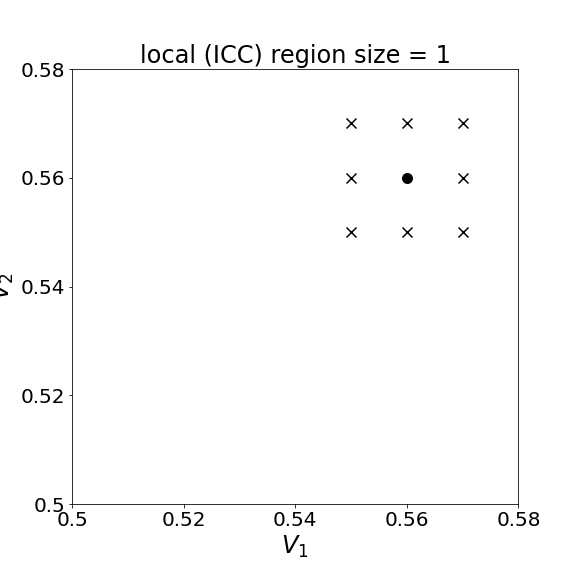
\includegraphics[width=0.3\textwidth]{images/local_size_1.png}
    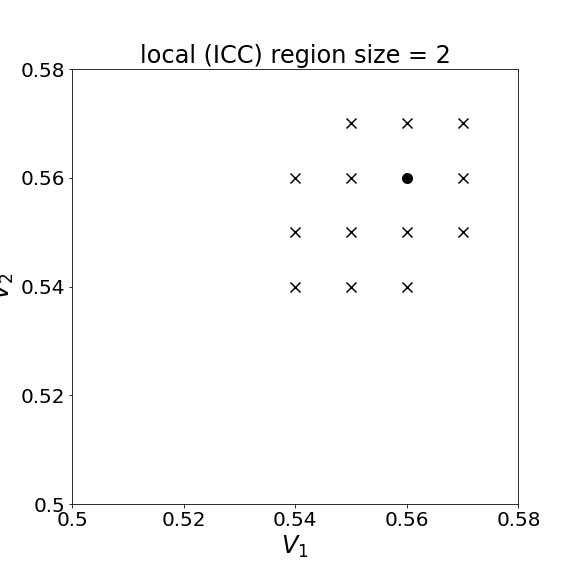
\includegraphics[width=0.3\textwidth]{images/local_size_2.png}
    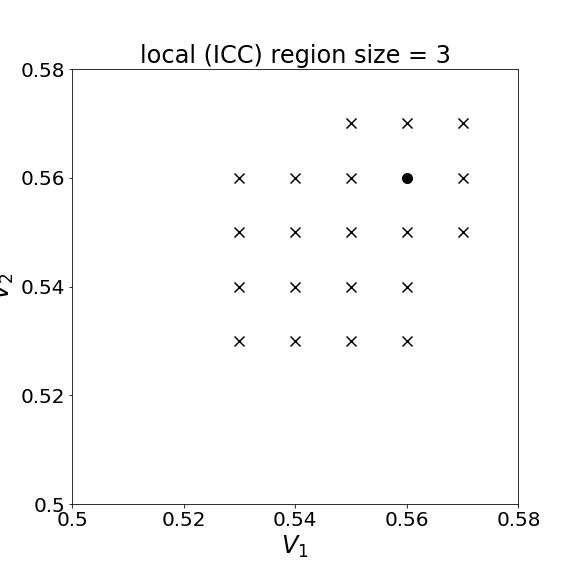
\includegraphics[width=0.3\textwidth]{images/local_size_3.png}
    \end{center}
    
    \vspace{1mm}
    \raggedright{\small {\sc Figure \refstepcounter{fig}\thefig\label{fig:sim1}:} We iteratively grow the local region of the discretized type space checked for downwards-sloping constraint violations. Notice that immediately adjacent (ICC) constraints are always checked ($\times$) when the local region increases in size around a point ($\bullet$).}
\end{figure}


Belloni et al. \autocite*{belloni2010multidimensional} use a plane-putting algorithm which works with a randomly chosen subset of incentive-compatibility (ICC) and Border (B) constraints at each iteration. They provide an efficient reduction in the growth in $T$ of the Border constraints (B) from $O(2^{T^J})$ to $O(T^J \log(T^J))$ \autocite[Lemma 10]{belloni2010multidimensional}. We adopt their solution to checking (B) constraints; however, our approach to checking (ICC) constraints involves iteratively growing the `local' region of the type space around each point $v$ in the discretized set of types $V_T$. We do two things. First, all the immediately adjacent points in the discretized type space are always checked for incentive compatibility. Secondly, downwards-sloping points in the discretized type space are also checked. Furthermore, the downwards-sloping region of the type space grows until all (ICC) constraints are ultimately satisfied. This procedure is illustrated visually in Figure \ref{fig:sim1}. Thus, for a fixed-size local region around each point in the discretized type space, we first satisfy \textit{local} (ICC) and (B) constraints as in the iterative plane-cutting algorithm of \autocite{belloni2010multidimensional}. Then we run the separation oracle with \textit{all} (ICC) and (B) constraints. We then restart the solver with any previously violated constraints, this time increasing the size of the local region around each point in the discretized type space. This procedure iterates until no constraints are violated. This modified version of \autocite{belloni2010multidimensional}'s algorithm is described in Algorithm \ref{alg:1}.

\begin{figure}[t]
  \centering
  \begin{minipage}{.7\linewidth}
    \begin{algorithm}[H]
    \caption{Iterative plane-cutting algorithm with local and downwards-sloping (ICC) constraints}\label{alg:1}
    \SetAlgoLined
    % \KwData{$x=1$}
    % \KwResult{$y = x^n$}
    % $\text{local_size} = 1$\;
    $L = 1, S = \emptyset, A = \emptyset, \overline{OPT} = \infty$\;
    \texttt{violated\_any\_icc} $\gets $ TRUE\; 
    \While{\texttt{violated\_any\_icc}}{
        \texttt{violated\_local\_icc} $\gets$ TRUE\; 
        \While{\texttt{violated\_local\_icc}}{
          $k = 1, A^k = A, S^k = S$\;
          Solve the linear program associated with $S^k$. Let $OPT^k$ denote the optimal value.\;
          Solve the separation oracle using only local (ICC) constraints in region $L$. Let $A^k$ denote all violated local (ICC) and (B) constraints.\;
          \If{$A^k = \emptyset$}{
            \texttt{violated\_local\_icc} $\gets$ FALSE\;
            Break\;
          }
          Select a subset $I^k \subset S^k$ of inactive (ICC) and (B) constraints\;
          \eIf{$OPT^k < \overline{OPT}$}{
            $S^{k+1} \gets (S^k \setminus I^k) \cup A^k \cup A$\;
            $\overline{OPT} \gets OPT^k$\;
          }{
            $S^{k+1} \gets S^k \cup A^k \cup A$\;
          }
          $k \gets k+1$\;
        }
        Solve the separation oracle using all (ICC) constraints. Let $A^*$ denote all violated (ICC) constraints.\;
        \If{$A^* = \emptyset$}{
            \texttt{violated\_any\_icc} $\gets$ FALSE\;
            Break\;
        }
        $A \gets A \cup A^*$\;
        $S \gets S^k$\;
        $L \gets L + 1$\;
    }
    \end{algorithm}
  \end{minipage}
\end{figure}

Our algorithm\footnote{For more details see: \url{https://github.com/jmemich/optimal-auction-multidim}} is written in Python 3.10 and uses Google's open source linear programming solver `GLOP' available in their \texttt{or-tools} package \autocite{ortools}.

\section{Census Non-Response Calculations}\label{appendix_census_calc}

The 2020 census post-enumeration survey data can be found in the US Census data tables\footnote{\url{https://data.census.gov/table}}, where the `Net Coverage Error for the Household Population in the United States by Race and Hispanic Origin' is given by the variable \textbf{C\_RACEHISUS} and the net coverage error is estimated at -4.99\%. The data for the 2010 US Census are not available on the census data tables, however, the official estimated net undercount of Hispanics was -1.54\% \autocite[p1]{census2010coverage}.




\end{document}
